\documentclass[11pt]{template/cauchy}
\usepackage[czech]{babel}

\usepackage{enumerate}
\usepackage{mlmodern}
\usepackage{template/mathsphystools}
\usepackage{amsthm,thmtools,xcolor,amsmath,amssymb}
\usepackage[scr]{rsfso}
% \usepackage{thmstyles}
\usepackage{tabularx}
\usepackage{graphicx}
\usepackage{multicol}
\usepackage{appendix}
\usepackage{tabularx}
\usepackage{subcaption}
\usepackage{hyperref}
\usepackage{comment}
\usepackage{lscape}
\graphicspath{{images/}}

\declaretheoremstyle[
  headfont=\color{red}\normalfont\bfseries,
  bodyfont=\color{black}\normalfont,
]{def}

\declaretheoremstyle[
  headfont=\color{blue}\normalfont\bfseries,
  bodyfont=\color{black}\normalfont\itshape,
]{pr}

\declaretheoremstyle[
  headfont=\color{green}\normalfont\bfseries,
  bodyfont=\color{black}\normalfont\itshape,
]{veta}

\declaretheoremstyle[
  headfont=\color{brown}\normalfont\bfseries,
  bodyfont=\color{black}\normalfont,
]{pozn}

\declaretheoremstyle[
  headfont=\color{brown}\normalfont\bfseries,
  bodyfont=\color{black}\normalfont,
]{dusl}

\declaretheorem[
  style=def,
  name=Definice,
]{definition}

\declaretheorem[
  style=pr,
  name=Příklad,
]{example}

\declaretheorem[
  style=veta,
  name=Věta,
]{veta}

\declaretheorem[
  style=pozn,
  name=Poznámka,
]{pozn}

\declaretheorem[
  style=dusl,
  name=Důsledek,
]{dusledek}

\DeclareMathOperator{\tg}{tg}
\DeclareMathOperator{\cotg}{cotg}
\DeclareMathOperator{\arctg}{arctg}
\DeclareMathOperator{\arccotg}{arccotg}

\title[Title for the Header]{Matematika}
\subtitle{}
\author{Dominik Doležel \& Honza Romanovský}
\affiliation{Gymnázium Brno, třída Kapitána Jaroše}
\date{\today}
\begin{document}

%!TEX root = ../main.tex
\setcounter{page}{0}
\thispagestyle{fancy-blank}
\begingroup
% \vphantom{Optional note}
{\large \par}
\vspace*{35mm}
{\huge\bfseries\utitle\par}

\vspace*{5mm}
{\Large\usubtitle\par}

\vspace*{4mm}
{\rule{\linewidth}{0.5mm}\par}
\vspace*{4mm}

{\large\bfseries\uauthor\par}\vspace*{1mm}

{\large\itshape\uaffiliation\newline}
{\large\itshape{Provizorní nápis}\par}

\vfill
{\large \par}
\endgroup
\clearpage


\frontmatter
\tableofcontents
\clearpage
% \listoffigures
% \listoftables
% \clearpage

% Každá otázka vypadá takto:
% \section*{Název otázky}
% \subsection{Základní pojmy}
% itemize se seznamem základních pojmů
% \section*{Příklady}

\mainmatter

% \input{01_nazev_otazky}

\section{Základní pojmy z teorie množin}
\begin{definition}
  \textbf{Množina} je sourhn objektů, chápaný jako celek. Tyto objekty nazýváme prvky množiny.
\end{definition}

Množina může být konečná, nekonečná nebo prázdná. Množinu lze zadat výčtem prvků nebo pomocí charakteristické vlastnosti (např. $\left \{ 2k, k \in \mathbb{N}\right\}$).

\begin{definition}
  \textbf{Podmnožina} množiny $A$ je taková množina $B$, že všechny její prvky patří do množiny $A$.
\end{definition}

Každá neprázdná množina má dvě \textbf{nevlastní podmnožiny}: množinu prázdnou a sebe sama. Všechny ostatní její podmnožiny nazýváme nevlastní.

\begin{definition}
  Množiny $A$ a $B$ se rovnají právě tehdy, když $A$ je podmnožinou $B$ a zároveň $B$ je podmnožinou $A$.
\end{definition}

\begin{definition}
  Nechť $A \subseteq B$ a $B\neq \emptyset$. Množinu všech prvků mn. $B$, které nepatří do mn. $A$, nazýváme \textbf{doplněk} (komplement) množiny $A$ v množině $B$. Značíme $A_B^\prime.$
\end{definition}

\begin{definition}
  Nechť $A, B$ jsou dvě množiny. Jejich \textbf{sjednocením} nazveme takovou množinu, která obsahuje ty prkvy, které patří alespoň do jedné z množin $A, B$. Zapisujeme $A \cup B.$
\end{definition}

----
Honzo neschovávej se už píšeme


průnik mn\\
vennovy diag \\
disjunktní mn\\
rozdíl mn\\
de morganova pravidla plus dk!!\\

\begin{pozn}[Číselné množiny]
  Rozlišujeme následující základní číselné množiny:
  \begin{itemize}
    \item $\mathbb{N}$: přirozená čísla $(1, 2, 3, \dots)$,
    \item $\mathbb{Z}$: celá čísla $(\dots, -2, -1, 0, 1, 2, \dots)$,
    \item $\mathbb{Q}$: racionální čísla $(3/5, 0,\overline{3})$,
    \item $\mathbb{R}$: reálná čísla $(e, \pi)$,
    \item $\mathbb{C}$: komplexní čísla $(3+2i)$
  \end{itemize}
\end{pozn}

Iracionální čísla ($\mathbb{I}$) jsou doplněk racionálních v $\mathbb{R}$.

\begin{definition}
  \textbf{Celá čísla} jsou čísla, která vyjadřují počty prvků množin, čísla k nim opačná a číslo 0.
\end{definition}

\begin{definition}
  \textbf{Racionálním číslem} nazveme takové číslo $a = \frac{k}{l}, k, l \in \mathbb{Z}$, a $p,q$ jsou nesoudělná.
\end{definition}

\begin{pozn}
  Přirozená čísla zapisujeme pomocí číslic 0--9 a chápeme je takto:
  $$4503=4\cdot 10^3+5\cdot 10^2 + 0 \cdot 10^1 + 3\cdot 10^0.$$
  Každé racionální číslo je v desítkové soutavě vyjádřeno buď nekonečným desetinným rozvojem nebo neukončeným periodickým rozvojem. Iracionální číslo je vyjádřeno neukončeným neperiodickým rozvojem.
\end{pozn}

\begin{definition}
  \textbf{Reálnými čísly} nazýváme všechna čísla, která jsou velikostmi úseček.
\end{definition}

\begin{definition}
  Nechť $a,b \in \mathbb{R},$ kde $a<b$. Pak množiny takových $x\in \mathbb{R},$ že $a\leq x\leq b$ (resp. $a < x < b$, resp. $a < x$, resp. $a \leq x < b$ atd.) nazýváme uzavřeným (resp. otevřeným, resp. neomezeným zleva otevřeným, resp.zprava uzavřeným, zleva otevřeným atd.) \textbf{intervalem}. Zapisujeme $\left<a,b\right>$ (resp. $\left(a,b\right)$, resp. $(a, \infty)$, resp. $\left<a, b\right)$)
\end{definition}

für Honza: periodický rozvoj čísel, množina komplexních čísel, imaginární čísla -- něco z toho už možná je, nevim

\begin{example}[SÚM 169/8]
  Označme $M$ množinu všech dvojciferných přirozených čísel delitelných šesti a $N$ všechn dělitelů čísla 210, kteří jsou různí od čísla 1 a 210. Určete, která z množin má větší počet prvků, a vypište všechny prvky, které mají obě množiny stejné.
  \begin{align*}
    M & = \left\{12, 18, 24, 30, 36, 42, 48, 54, 60, 66, 72, 78, 84, 90, 96\right\}\\
    210 & = 2\cdot 3 \cdot 5  \cdot 7 \textrm{ -- hledáme násobky všech podmnožin těchto čísel} \\
    N  & = \left\{2,3,5,6,7, 10, 14, 15, 21, 30, 35, 42, 70, 105\right\} \\
    |M| & = 15, |N| = 14, M \cap N = \left\{30, 42\right\}
  \end{align*}

  \rm Množina $M$ má více prvků a společná jsou čísla 30 a 42.
\end{example}

\begin{example}[SÚM 171/26]
  $M$ je množina šech reálných čísel $x$, která splňují nerovnosti $-2<x<5$, $N$ je mn. všech reálných čísel $y$, která splňují nerovnost $|y|<4$. Určete množinu $R=M\cup N$ a $S = M\cap N.$ \hfill $R = (-4,5), S=(-2,4).$
\end{example}

\begin{example}[SÚM 172/29f]
  Znázorněte a určete výsledný interval: $(a,a+2)\cap (a-1,a+1),$ kde $a>0.$\hfill$(a,a+1)$
\end{example}

\begin{example}[SÚM (172/33)]
  Je dána kružnice $k$ se středem v bodě  $S$ a poloměrem $r$. Množinu všech bodů uvnitř kružnice označte $A$. Nakreslete rovnostranný trojúhelník $ESD$, jehož jeden vrchol je ve středu dané kružnice a délky stran jsou rovny velikosti jejího průměru. Množinu vnitřních bodů tohoto trojúhelníka ozn. $B$. Díle sestrojte osu úhlu $ESD$ a množinu bodů této přímky označte $C$. Nakreslete samostatné obrázky pro:
  \begin{itemize}
    \item $(A\cap B)\cup C,$
    \item $(A\cup C) \cap (B\cup C),$
    \item $(A\cap B) \cup (B\cap C),$
    \item $(A\cup C) \cap B$.
  \end{itemize}
\end{example}

\begin{example}[SÚM 173/34]
  Pro která $x$ je interval:
  \begin{enumerate}[a.]
    \item $\left<2x,x+3\right>$ částí intervalu $(2,7)$? \hfill $x \in (1,3)$
    \item $(x,5)$ částí intervalu $\left(-1,x+1\right)$? \hfill $x\in (4,5)$
    \item $(x,x+3)$ částí intervalu $\left<5,8\right>$? \hfill $x=5$
    \item $\left<x,2x-1\right>$ částí intervalu $\left<-2,5\right>$? \hfill $x\in\left<-2,5\right>$
    \item $\left<3x,2x+1\right>$ částí intervalu $(3,6)$? \hfill $x\in \left\{\right\}$
  \end{enumerate}
\end{example}

\begin{example}[SÚM 173/35]
  Nechť $M = (a,b), N = (1,8), Q = (1,5)$. Určete $a,b \in \mathbb{R}$ tak, aby platilo $M\cap N = Q$.\hfill $a\in \left(-\infty, 1\right>, b=5$
\end{example}

\begin{example}[SÚM 173/37*]
  Je dán trojúhelník $ABC$. Uvažujme množinu $M$ všech bodů tohoto trojúhelníka, pro které platí $|AX| \geq |BX| \geq |CX|.$ Pomocí velikosti stran a úhlů troj. $ABC$ vyjádřete podmínky pro to, aby:
  \begin{enumerate}[a.]
    \item $X$ byla pětiúhelník, \hfill $\gamma > 90^\circ, \alpha < \beta$
    \item $X$  je jeden bod, \hfill $\alpha = 90^\circ$
    \item $X$ je prázdná.\hfill $\alpha > 90^\circ$
  \end{enumerate}
\end{example}


\begin{example}[SÚM 174/42]
  Jsou dány množiny $M=\left\{1,2;3;4\right\},N=\left\{x;y;z\right\}.$ Uveďte alespoň jeden příklad na zobrazení množiny
  \begin{enumerate}[a.]
    \item $M$ do $N$\hfill $1,2\rightarrow x, 3\rightarrow y, 4 \rightarrow y$
    \item $N$ do $M$ \hfill $x\rightarrow 1,2, y\rightarrow 3, z\rightarrow 3$
    \item $M$ na $N.$ \hfill $1,2\rightarrow x, 3 \rightarrow y, 4 \rightarrow z$
  \end{enumerate}
\end{example}

\begin{example}[SÚM 174/46]
  Kolik je všech zobrazení (pod)množiny $\left\{a,b,c,d\right\}$ do (na) množiny $\left\{1,2\right\}$?\hfill \rm 81
\end{example}

\begin{example}[SÚM 106/20]
  Převeďte na obyčejné zlomky:
  \begin{enumerate}[a.]
    \item $0,\overline{27}$\hfill $\frac{27}{99}\frac{3}{11}$
    \item $0,\overline{6}$ \hfill $\frac{2}{3}$
    \item $2,\overline{345}$ \hfill $2+\frac{345}{999}=\frac{781}{333}$
    \item $0,\overline{1234}$\hfill $\frac{1234}{9999}$
    \item $0,7\overline{2}$\hfill $\frac{7}{10}+\frac{2}{90}=\frac{13}{18}$
    \item $0,1\overline{36}$\hfill $\frac{1}{10}+\frac{36}{990}=\frac{3}{22}$
    \item $0,7\overline{27}$\hfill $\frac{7}{10}+\frac{27}{990}=\frac{8}{11}$
    \item $3,39\overline{85}$\hfill $3+\frac{39}{100}+\frac{85}{9900}=\frac{33646}{9900}$
  \end{enumerate}
\end{example}

\begin{example}[SÚM 107/21]
  Proveďte:
  \begin{enumerate}[a.]
    \item $0,\overline{4}+0,\overline{12}$ \hfill $\frac{4}{9}+\frac{12}{9}=\frac{16}{9}$
    \item $0,\overline{7}+0,\overline{35}$  \hfill $\frac{112}{99}$
    \item $0,\overline{47}+0,\overline{023}$ \hfill $\frac{5470}{10989}$
    \item $0,\overline{47}+0,0\overline{23}$ \hfill $\frac{493}{990}$
    \item $0,5\overline{354}+0,\overline{85}$\hfill $1,394021\dots$
    \item $2,\overline{35}-1,\overline{231}$\hfill$ \frac{4111}{3663}$
    \item $1,\overline{25}-0,\overline{773}$ \hfill $\frac{5261}{10989}$
  \end{enumerate}

\begin{example}[SÚM 107/22*]
  Proveďte:
  \begin{enumerate}[a.]
    \item $1,\overline{2}\cdot 1,\overline{18}$\hfill $\left(1+\frac{2}{9}\right)\left(1+\frac{18}{99}\right)=\frac{11}{9}\cdot \frac{117}{99}=\frac{13}{9}$
    \item $0,\overline{32}\cdot 1,\overline{3}$\hfill $\frac{128}{297}$
  \end{enumerate}
\end{example}

\begin{example}[SÚM 107/23*]
  Řešte rovnici:
  \begin{enumerate}
    \item $0,\overline{25}x + 0,\overline{31}x = 1,\overline{13}$ \hfill $x=2$
    \item $2,\overline{64}x - 3,\overline{48} = 1,\overline{48}$  \hfill $x = 3$
  \end{enumerate}
\end{example}

končím ruším nesleduju tě

\end{example}

\section{Výroková logika}
\begin{definition}
  \textbf{Výrokem} nazýváme každou oznamovací větu, která je buď pravdivá, nebo nepravdivá. \textbf{Pravdivostní hodnotou} výroku rozumíme jeho pravdivost / nepravdivost.
\end{definition}

\begin{definition}
  \textbf{Negací výroku} $V$ nazýváme výrok $V^\prime$, který má opačnou pravdivostní hodnotu než výrok $V$.
\end{definition}

\begin{pozn}
  \textbf{Kvantifikované výroky} jsou výroky, které uvádějí počet objektů. Pro to lze použít
  \begin{itemize}
    \item obecný kvantifikátor $\forall$ (pro všechno platí),
    \item existenční kvantifikátor $\exists$ (existuje alespoň jeden, že pro něj platí) a
    \item zesílený existenční kvantifikátor $\exists !$ (existuje právě jeden, že pro něj platí) a
  \end{itemize}
\end{pozn}

\begin{definition}
  \textbf{Složeným výrokem} rozumíme více výroků spojených logickými spojkami:
  \begin{center}
    \begin{tabular}{l | c c}
      název & zápis & význam \\
      \hline
      negace & $X^\prime$ & není pravda, že \\
      konjunkce & $X\land Y$ & $X$ a $Y$ platí současně \\
      alternativa & $X\lor Y$ & platí alespoň jedno z $X,Y$\\
      implikace & $X\implies Y$ & jestliže $X$, pak $Y$\\
      ekvivalence & $X\iff Y$ & $X$ platí právě tehdy, když platí $Y$
    \end{tabular}
  \end{center}
\end{definition}


\begin{pozn}
  Pravdivostní hodnoty výrokových formulí s logickou spojkou:
  \begin{center}
    \begin{tabular}{c c | c c | c c c c}
      $X$ & $Y$ & $X^\prime$ & $Y^\prime$ & $X\land Y$ & $X\lor Y$ & $X\implies Y$ & $X\iff Y$ \\
      \hline
      1 & 1 & 0 & 0 & 1 & 1 & 1 & 1 \\
      1 & 0 & 0 & 1 & 0 & 1 & 0 & 0 \\
      0 & 1 & 1 & 0 & 0 & 1 & 1 & 0 \\
      0 & 0 & 1 & 1 & 0 & 0 & 1 & 1 \\
    \end{tabular}
  \end{center}
\end{pozn}

\begin{definition}
  Výrazy sestavené z výrokových proměnných, závorek a logických spojek nazýváme \textbf{výrokové formule}.
\end{definition}

\begin{definition}
  Výroková formule, která nabývá pravdivostní hodnoty 1 bez ohledu na pravdivostní hodnoty elementárních výroků, se nazývá \textbf{tautologie}.
\end{definition}

\begin{veta}
  Pro každé dva výroky $X,Y$ platí:
  \begin{enumerate}[$i.$]
    \item $(X\lor Y)^\prime = X^\prime \land Y^\prime$,
    \item $(X\land Y)^\prime = X^\prime \lor Y^\prime$,
    \item $(X\implies Y)^\prime = X\land Y^\prime$ a
    \item $(X\iff Y)^\prime = (X\land Y^\prime) \lor (X^\prime \land Y)$
  \end{enumerate}
\end{veta}

\begin{definition}
  Nechť $X\implies Y$ je implikace. Pak
  \begin{enumerate}[$i.$]
    \item implikaci $Y\implies X$ nazýváme \textbf{obrácením} a
    \item implikaci $Y^\prime \implies X^\prime$ nazýváme \textbf{obměnou}
  \end{enumerate}
  původní implikace.
\end{definition}

\begin{veta}
  Implikace a její obměna mají touž pravdivostní hodnotu.
\end{veta}

\begin{pozn}
  Implikace a její obrácení nemusí vždy mít touž pravdivostní hodnotu.
\end{pozn}

\begin{definition}
  \textbf{Výroková forma} je tvrzení obsahující proměnné. Po dosazení konstant za proměnné dostáváme výrok.
\end{definition}

\begin{pozn}
  Důležitému netriviálnímu a dostatečně obecnému výroku nebo výrokové formě s matematickým obsahem říkáme \textbf{věta}.
\end{pozn}

\begin{example}[SMP 143/4]
  Jsou následující výroky tautologie?
  \rm
  \begin{enumerate}[a.]
    \item $\left[(A\implies B)\land A\right]\implies B$
    \begin{center}
      \begin{tabular}{c c | c c c}
        $A$ & $B$ & $A \implies B$ & $(A\implies B)\land A$ & $(A\implies B)\land A]\implies B$ \\
        \hline
        1 & 1 & 1 & 1 & 1 \\
        1 & 0 & 0 & 0 & 1 \\
        0 & 1 & 1 & 0 & 1 \\
        0 & 0 & 1 & 0 & 1
      \end{tabular}
    \end{center}
    Výrok je tautologií.
    \item $\left[(A\implies B)\land B^\prime\right]\implies A^\prime$
    \begin{center}
      \begin{tabular}{c c c c | c c c}
        $A$ & $B$ & $A^\prime$ & $B^\prime$ &  $A \implies B$ & $(A\implies B)\land B^\prime$ & $\left[(A\implies B)\land B^\prime\right]\implies A^\prime$ \\
        \hline
        1 & 1 & 0 & 0 & 1 & 0 & 1 \\
        1 & 0 & 0 & 1 & 0 & 0 & 1 \\
        0 & 1 & 1 & 0 & 1 & 0 & 1 \\
        0 & 0 & 1 & 1 & 1 & 1 & 1
      \end{tabular}
    \end{center}
    Výrok je tautologií.
  \end{enumerate}
\end{example}

\begin{example}[SMP 144/8]
  Na modelu kolejiště je možno uvést do pohybu tři vlakové soupravy A,B,C. V daném okamžiku je jejich
situace charakterizována formulí $$\left[(A^\prime \lor B^\prime) \implies C\right]\land\left[(A \lor C) \implies B^\prime\right].$$ Které soupravy jsou v pohybu?

\rm Napišme tabulku pravdivostních hodnot.
\begin{center}
  \begin{tabular}{c c c c c | c c c c c}
    $A$ & $B$ & $C$ & $A^\prime$ & $B^\prime$ & $A^\prime \lor B^\prime$ & $(A^\prime \lor B^\prime) \implies C$ & $A\lor C$ & $(A \lor C) \implies B^\prime $ & celkem\\
    \hline
    1 & 1 & 1 & 0 & 0 & 0 & 1 & 1 & 0 & 0 \\
    1 & 1 & 0 & 0 & 0 & 0 & 1 & 1 & 0 & 0 \\
    1 & 1 & 0 & 0 & 0 & 1 & 1 & 1 & 1 & 1 \\
    1 & 0 & 1 & 0 & 1 & 1 & 0 & 1 & 1 & 0 \\
    0 & 1 & 1 & 1 & 0 & 1 & 1 & 1 & 0 & 0 \\
    0 & 1 & 0 & 1 & 0 & 1 & 0 & 0 & 1 & 0 \\
    0 & 0 & 1 & 1 & 1 & 1 & 1 & 1 & 1 & 1 \\
    0 & 0 & 0 & 1 & 1 & 1 & 0 & 0 & 0 & 0
  \end{tabular}
\end{center}
Buď jsou v provozu soupravy $A$ a $C$ nebo jen souprava $C$.
\end{example}

\begin{example}[SMP 144/10]
  Květa si pozvala na oslavu svých osmnáctin přátele. Uvažuje takto:
  \begin{enumerate}[a.]
    \item Alena a Boris chodí vždycky spolu. Přijdou oba, nebo ani jeden.
    \item Přijde Boris nebo Dan, ale určitě ne oba.
    \item Když přijde Alena, pak přijde i Eva.
    \item Když Eva nepřijde, nepřijde Dan.
  \end{enumerate}
  S jakým největším počtem přátel může Květa počítat? Vyplývá z Květiny úvahy, že může nastat situace, kdy nepřijde ani jeden z pozvaných?

  \rm Přeložme tato tvrzení symbolicky.
  \begin{enumerate}[a.]
    \item $A\iff B$
    \item $(B^\prime \land D) \lor (B \land D^\prime)$
    \item $A\implies E$
    \item $E^\prime \implies D^\prime$
  \end{enumerate}
  Protože alespoň jeden z dvojice Boris, Dan nemůže přijít a zbytek podmínek si neodporují, na oslavu můžou přijít nejvýše tři lidé.

  Situace, že nepřijde nikdo nastat nemůže, protože výdy přijde buď Boris, nebo Dan.
\end{example}

\begin{example}[SMP 144/12]
  Trenér se věnuje trojici gymnastů -- Adamovi, Břéťovi a Čeňkovi. Rozhodněte, koho vyšle na kontrolní
závod, jestliže splní tyto tři podmínky:
\begin{itemize}
  \item Tělovýchovnou jednotu budou reprezentovat nejvýše dva závodníci, přitom pojede aspoň jeden.
  \item Pojede Adam nebo Čeňek, ale určitě ne oba součastně.
  \item Nepojede-li Čeňek, pak nepojede ani Břéťa.
\end{itemize}

\rm Rozdělme příklad na dva případy.
\begin{enumerate}[$i.$]
  \item pojede Adam: pak nepojede Čeněk a tedy ani Břéťa,
  \item pojede Čeněk: pak může jet i Břéťa.
\end{enumerate}

Buď pojede Adam sám nebo Čeněk sám nebo Čeněk s Břéťou.

\end{example}

\begin{example}[SMP 143/13]
  V souvislosti s otevřením další části metra uvažuje komise o účelnosti autobusových linek A, B, C, D. Je přitom třeba vzít v úvahu tyto tři skutečnosti:
  \begin{itemize}
    \item  Aspoň jedna z linek A, B, C bude zrušena.
    \item Bude-li zrušena linka A, pak bude zachována linka B nebo D.
    \item Nebude-li zrušena linka C, pak bude zrušena linka A nebo D.
  \end{itemize}
  Najděte všechna řešení a rozhodněte, zda stačí zachovat jen jednu z linek.

  \rm Pokud linka $X$ jezdí, píšeme $X$, v opačném případě $X^\prime.$ Podmínky převedeme jako:
  \begin{itemize}
    \item $A^\prime\lor B^\prime \lor C^\prime$
    \item $A^\prime \implies (B\lor D)$
    \item $C\implies (A^\prime\lor D^\prime)$
  \end{itemize}
  Sestavme tabulku (\uv{celkem} značí konkunkci všech tří podmínek výše):
  \begin{widetext}
    \begin{center}
      \begin{tabular}{c c c c | c c c c c | c}
        $A$ & $B$ & $C$ & $D$ & $A^\prime\lor B^\prime \lor C^\prime$ & $B\lor D$ & $A^\prime \implies (B\lor D)$ & $A^\prime \lor D^\prime$ & $C\implies (A^\prime\lor D^\prime)$ & celkem \\
        \hline
        1 & 1 & 1 & 1 & 0 & 1 & 1 & 0 & 0 & 0 \\
        1 & 1 & 1 & 0 & 0 & 1 & 1 & 1 & 1 & 0 \\
        1 & 1 & 0 & 1 & 1 & 1 & 1 & 0 & 0 & 0 \\
        1 & 1 & 0 & 0 & 1 & 1 & 1 & 1 & 1 & 1 \\
        1 & 0 & 1 & 1 & 1 & 1 & 1 & 0 & 0 & 0 \\
        1 & 0 & 1 & 0 & 1 & 0 & 1 & 1 & 0 & 1 \\
        1 & 0 & 0 & 1 & 1 & 1 & 1 & 0 & 1 & 0 \\
        1 & 0 & 0 & 0 & 1 & 0 & 1 & 1 & 1 & 1 \\
        0 & 1 & 1 & 1 & 1 & 1 & 1 & 1 & 1 & 1 \\
        0 & 1 & 1 & 0 & 1 & 1 & 1 & 1 & 1 & 1 \\
        0 & 1 & 0 & 1 & 1 & 1 & 1 & 1 & 1 & 1 \\
        0 & 1 & 0 & 0 & 1 & 1 & 1 & 1 & 1 & 1 \\
        0 & 0 & 0 & 1 & 1 & 1 & 1 & 1 & 1 & 1 \\
        0 & 0 & 1 & 0 & 1 & 0 & 0 & 1 & 1 & 0 \\
        0 & 0 & 1 & 1 & 1 & 1 & 1 & 1 & 1 & 1 \\
        0 & 0 & 0 & 0 & 1 & 0 & 0 & 1 & 1 & 0 \\
      \end{tabular}
    \end{center}
  \end{widetext}
  Výsledek je patrný z tabulky. Může nastat situace, že bude jezdit jediná linka, a to buď $A$, nebo $D$.
\end{example}

\begin{example}[ŘMÚ 274/28.5]
  \begin{enumerate}[a.]
    \item K implikaci \uv{jestliže funkce $f$ má v každém bodě intervalu $(a,b)$ kladnou derivaci, pak funkce $f$ je v intervalu $(a,b)$ rostoucí} utvořte negaci, obměněnou a obrácenou implikaci a stanovte jejich pravdivostní hodnoty.

    {\rm negace: \uv{funkce $f$ má v každém bodě intervalu $(a,b)$ kladnou derivaci a funkce $f$ není v intervalu $(a,b)$ rostoucí}, obměna: \uv{jestliže funkce $f$ není v intervalu $(a,b)$ rostoucí, pak funkce $f$ alespoň v jednom bodu intervalu $(a,b)$ nemá kladnou derivaci}, obrácení: \uv{jestliže funkce $f$ je v intervalu $(a,b)$ rostoucí, pak funkce $f$ má v každém bodě intervalu $(a,b)$ kladnou derivaci}}
    \item Negujte výroky:
    \begin{enumerate}[1.]
      \item Aspoň jeden příklad jsem vyřešil správně.
      \item V tomto sadě je aspoň dvacet jabloní.
      \item Nejvýše šest žáků naší třídy prospělo s vyznamenáním.
      \item Každý den vstávám v sedm hodin.
    \end{enumerate}
    \vspace{3em}
    {\rm
      \begin{enumerate}[1.]
        \item Všechny příklady jsem vyřešil špatně.
        \item V tomto sadě je nejvýše devatenáct jadbloní.
        \item Alespoň sedm žáků naší třídy prospělo s vyznamenáním.
        \item Alespoň v jeden den nevstávám v sedm hodin.
      \end{enumerate}
    }
    \item Když si dám kávu, dám si i moučník. Nedám-li si zmrzlinu, nedám si moučník.
    \begin{enumerate}[1.]
      \item Vyplývá z uvedeného, že dám-li si zmrzlinu, pak si nedám kávu?\hfill {\rm ne}
      \item Vyplývá z uvedeného, že když si dám kávu, dám si i zmrzlinu?\hfill {\rm ano}
    \end{enumerate}
  \end{enumerate}
\end{example}

\begin{example}[ŘMÚ 275/28.6]
  \begin{enumerate}[a.]
    \item K implikaci \uv{Je-li dané přirozené číslo dělitelné dvěma a zároveň třemi, pak je dělitelné šesti}  utvořte
negaci, obměněnou a obrácenou implikaci.
\item Nebude-li ráno pršet, pojedeme na chalupu. Zjišťujeme, že ráno prší. Usuzujeme správně, když z uvedeného
odvodíme, že na chalupu nepojedeme?
\item Pro práci strojů A, B, C platí dvě podmínky: Nesmí pracovat pouze stroj B. Když pracuje stroj A, pak musí
být v chodu i stroj B. Navrhněte síť, která bude pro tuto trojici strojů kontrolním zařízením a bude
signalizovat nesplnění aspoň jedné z uvedených podmínek.
  \end{enumerate}
  \vspace{3em}
  \rm
  \begin{enumerate}[a.]
    negace: \uv{Dané přirozené číslo je dělitelné dvěma a zároveň třemi a není dělitelné šesti}, obměna: \uv{Jetliže dané přirozené číslo není dělitelné šesti, pak není dělitelné dvojkou nebo trojkou}, obrácení: \uv{Jestliže je dané přirozené číslo dělitelné šesti, pak je dělitelné dvěma a třemi}.
    \item ne
    \item Podmínky lze zapsat jako:
      $$B\implies (A\lor C), A\implies B.$$
    Z tabulky pravdivostních hodnot lze vyvodit, že nevyhovují jen možnosti $A, B^\prime, C$ a $A, B^\prime, C^\prime$.
  \end{enumerate}
\end{example}

\begin{example}[SÚM 240/1]
  Počet úhlopříček vypuklého $n$-úhelníka se vypočítá podle vzorce $P_n=\frac{n(n-3)}{2},$ kde $n$ je přirozené číslo větší než tři. Dokažte jeho správnost matematickou indukcí.

  \rm \begin{enumerate}[$i.$]
    \item $n=4:$
    $$P_4 = \frac{4(4-3)}{2}=2 \rightarrow \textrm{platí}$$
    \item úvaha: Přidáním $n$-tého bodu se zvýší počet úhlopříček o $n-3$ (úhlopříčky mezi novým bodem a těmi starými, se kterými nemá společnou stranu) a $1$ (strana, jejíž koncové body jsou ty body, se kterými má $n$-tý bod společnou stranu, se přemění v úhlopříčku) $\rightarrow$ celkem přibyde $n-2$ úhlopříček. \\
    Chceme: $P_n=\frac{n(n-3)}{2}\implies P_{n+1}=\frac{(n+1)(n-2)}{2}$. Předpokládejme, že $P_n=\frac{n(n-3)}{2}$.

    \begin{align*}
      P_{n+1} & =P_n + (n-1) = \frac{n(n-3)}{2}+n-1 \\
      & =\frac{n(n-3)+2n-2}{2} = \frac{n^2-n-2}{2}\\
      & = \frac{(n+1)(n-2)}{2} \rightarrow \textrm{platí}
    \end{align*}
\end{enumerate}
\end{example}

\begin{example}[SÚM 240/5]
  Dokažte matematickou indukcí, že číslo $Q_n=5^{n+1}+6^{2n-1}$ je dělitelné číslem 31 pro každé přirozené číslo $n$.

  \rm \begin{enumerate}[$i.$]
    \item $n=1:$
    $$Q_1=5^2+6^1=31 \rightarrow \textrm{platí}$$
    \item chceme: $31 \, | \, Q_n \implies 31 \, | \, Q_{n+1}$. Předpokládejme, že $31 \, | \, Q_n.$

    \begin{align*}
      Q_{n+1}&=5^{n+2}+6^{2(n+1)-1}=5^{n+2}+6^{2n+1}\\
      & = 5\cdot 5^{n+2} + 6^{2n+1} = 5V_n - 5\cdot 6^{2n-1}+6^{2n+1} \\
      & = 5V_n + 6 ^{2n-1}(6^2-5)=5V_n + 31 \cdot 6^{2n-1} \rightarrow \textrm{platí}
    \end{align*}
\end{enumerate}
\end{example}

\begin{example}[SÚM 241/8]
  Dokažte, že součet třetích mocnin tří po sobě jdoucích přirozených čísel je dělitelný devíti.

  \rm Zapišme součet tří po sobě jdoucích přirozených čísel jako $a_n = (a-1) ^3 + a^3 + (a+1)^3 = 3a^3+6a.$
  \begin{enumerate}[$i.$]
    \item $a = 2:$
    $$a_2 = 1^3 + 2^3 + 3 ^3 = 36 \rightarrow \textrm{platí}$$
    \item chceme: $9\, | \, a_n \implies 9 \, | \, a_{n+1}$. Předpokládejme, že $9\, | \, a_n.$
    \begin{align*}
      a_{n+1} & = a^3 + (a+1)^3 + (a+2)^3 = \\
      & = a^3 + a^3 + 3a^2 + 3a + 1 + a^3 + 3\cdot 2\cdot a^2 + 3\cdot a\cdot 2^2 + 2^3\\
      &= 3a^3 + 9a^2 + 15a+9\\
      &= a_n + 9a^2 + 9a+ 9 = a_n + 9(a^2+a+1) \rightarrow \textrm{platí}
    \end{align*}
\end{enumerate}
\end{example}

\begin{example}[SÚM 241/9]
  Dokažte matematickou indukcí, že číslo $V_n = n^3 + 11n$ je dělitelné šesti pro každé přirozené číslo n.
  \begin{enumerate}[$i.$]
    \item $a = 1:$
    $$a_1 = 1^3 + 11\cdot1 = 12 \rightarrow \textrm{platí}$$
    \item chceme: $6\, | \, V_n \implies 6 \, | \, V_{n+1}$. Předpokládejme, že $6\, | \, V_n$.
    \begin{align*}
      V_{n+1} & = (n+1)^3 + 11\cdot(n+1) = \\
      & = n^3 + 3n^2 + 3n + 1 + 11n + 11\\
      &= n^3 + 11n + 3n^2 + 3n + 12\\
      &= V_n + 3n^2 + 3n + 12 = V_n + 12+ 3n(n+1) \rightarrow \textrm{platí}
    \end{align*}
\end{enumerate}
\end{example}

\begin{example}[SÚM 242/18]
  Matematickou indukcí dokažte tyto vzorce:
\begin{enumerate}[a.]
  \item $\frac{1}{1\cdot3}+\frac{1}{3\cdot5}+...+\frac{1}{(2n-1)\cdot(2n+1)} = \frac{n}{2n+1}$
    \begin{enumerate}[$i.$]
      \item $a = 1:$
      $$a_1 = \frac{1}{1\cdot3} = \frac{1}{2\cdot1 + 1}\rightarrow \textrm{platí}$$
      \item chceme: $S_n = \frac{n}{2n+1} \implies S_{n+1} = \frac{n+1}{2n+3}$. Předpokládejme, že $S_n = \frac{n}{2n+1}$.
      \begin{align*}
        S_{n+1} & = S_n + \frac{1}{(2n+1)\cdot(2n+3)} = \\
        & = \frac{n}{2n+1} + \frac{1}{(2n+1)\cdot(2n+3)}\\
        &= \frac{n\cdot(2n+3)+1}{(2n+1)\cdot(2n+3)}\\
        &= \frac{2n^2+3n+1}{(2n+1)\cdot(2n+3)} = \frac{(2n+1)\cdot(n+1)}{(2n+1)\cdot(2n+3)} = \frac{n+1}{2n+3} \rightarrow \textrm{platí}
      \end{align*}
    \end{enumerate}
  \item $\frac{1}{1\cdot4} + \frac{1}{4\cdot7}+...+\frac{1}{(3n-2)(3n+1)} = \frac{n}{3n+1}$
    \begin{enumerate}[$i.$]
      \item $a = 1:$
      $$a_1 = \frac{1}{1\cdot4} = \frac{1}{3\cdot1 + 1}\rightarrow  \textrm{platí}$$
      \item chceme: $S_n = \frac{n}{3n+1} \implies S_{n+1} = \frac{n+1}{3n+4}$. Předpokládejme, že $S_n = \frac{n}{3n+1}$.
      \begin{align*}
        S_{n+1} & = S_n + \frac{1}{(3n+1)(3n+4)} = \\
        & = \frac{n}{3n+1} + \frac{1}{(3n+1)(3n+4)}\\
        &= \frac{n\cdot(3n+4)+1}{(3n+1)(3n+4)}\\
        &= \frac{3n^2+4n+1}{(3n+1)(3n+4)} = \frac{(3n+1)(n+1)}{(3n+1)(3n+4)} = \frac{n+1}{3n+4} \rightarrow \textrm{platí}
      \end{align*}
    \end{enumerate}
  \item $\frac{1}{1\cdot 5}+ \frac{1}{5\cdot9}+...+\frac{1}{(4n-3)(4n+1)} = \frac{n}{4n+1}$
    \begin{enumerate}[$i.$]
      \item $a = 1:$
      $$a_1 = \frac{1}{1\cdot5} = \frac{1}{4\cdot1 + 1}\rightarrow  \textrm{platí}$$
      \item chceme: $S_n = \frac{n}{4n+1} \implies S_{n+1} = \frac{n+1}{4n+5}$. Předpokládejme, že $S_n = \frac{n}{4n+1}$.
      \begin{align*}
        S_{n+1} & = S_n + \frac{1}{(4n+1)(4n+5)} = \\
        & = \frac{n}{4n+1} + \frac{1}{(4n+1)(4n+5)}\\
        &= \frac{n\cdot(4n+5)+1}{(4n+1)(4n+5)}\\
        &= \frac{4n^2+5n+1}{(4n+1)(4n+5)} = \frac{(4n+1)(n+1)}{(4n+1)(4n+5)} = \frac{n+1}{4n+5} \rightarrow \textrm{platí}
      \end{align*}
    \end{enumerate}
  \item $1^2 + 3^2 + 5^2 + ... + (2n-1)^2 = \frac{n(2n-1)(2n+1)}{3}$
    \begin{enumerate}[$i.$]
      \item $a = 1:$
      $$a_1 = 1^2 = \frac{1\cdot1\cdot3}{3}\rightarrow  \textrm{platí}$$
      \item chceme: $S_n = \frac{n(2n-1)(2n+1)}{3} \implies S_{n+1} = \frac{(n+1)(2n+1)(2n+3)}{3}$. Předpokládejme, že $S_n = \frac{n(2n-1)(2n+1)}{3}$.
      \begin{align*}
        S_{n+1} & = S_n + (2n-1)^2 = \\
        & = \frac{n(2n-1)(2n+1)}{3} + \frac{12n^2-12n+3}{3}\\
        &= \frac{4n^3-n+12n^2-12n+3}{3}\\
        &= \frac{4n^3+12n^2-13n+3}{3} = \frac{(n+1)(2n+1)(2n+3)}{3} \rightarrow \textrm{platí}
      \end{align*}
    \end{enumerate}
    \item $1^3 + 2^3 + 3^3 + ... + n^3 = (\frac{n(n+1)}{2})^2$
      \begin{enumerate}[$i.$]
        \item $a = 1:$
        $$a_1 = 1^3 = (\frac{1\cdot2}{2})^2 \rightarrow  \textrm{platí}$$
        \item chceme: $S_n = (\frac{n(n+1)}{2})^2 \implies S_{n+1} =   (\frac{(n+1)(n+2)}{2})^2$. Předpokládejme, že $S_n = (\frac{n(n+1)}{2})^2$.
        \begin{align*}
          S_{n+1} & = S_n + n^3 = \\
          & = (\frac{n(n+1)}{2})^2 + \frac{4n^3}{4}\\
          &= \frac{n^4 + 2n^3 + n^2}{4} + \frac{4n^3}{4}\\
          &= \frac{n^4 + 6n^3 + n^2}{4} \rightarrow \textrm{neplatí?}
        \end{align*}
      \end{enumerate}
\end{enumerate}
\end{example}

\begin{example}[SÚM 242/19]

\end{example}

\begin{example}[SÚM 242/20]

\end{example}

\begin{example}[SMP 127/4]
  Matematickou indukcí dokažte Moivreovu větu: $(cos α + i sin α)^n = cos nα + i sin nα$.
  \begin{enumerate}[$i.$]
    \item $a = 1:$
    $$(cosø + isinø)^1 = cos(1ø) + isin(1ø)$$
    \item chceme: $S_n = (\frac{n(n+1)}{2})^2 \implies S_{n+1} =   (\frac{(n+1)(n+2)}{2})^2$. Předpokládejme, že $S_n = (\frac{n(n+1)}{2})^2$.
    \begin{align*}
      (cosø + isinø)^k = cos(kø) + isin(kø). (cosø + isinø)^{k+1} = cos((k + 1)ø) + isin((k + 1)ø).
   (cosø + isinø)^{k+1} = (cosø + isinø)^k x (cosø + isinø)
        = (cos(kø) + isin(kø)) x (cosø + isinø)
                 = cos(kø)cos(ø) + icos(kø)sin(ø) + isin(kø)cos(ø) - sin(kø)sin(ø)
                 = cos(kø + ø) + isin(kø + ø)
                = cos((k + 1)ø) + isin((k + 1)ø) \rightarrow \textrm{platí}
    \end{align*}
  \end{enumerate}
\end{example}

\begin{example}

\end{example}

\section{Dělitelnost přirozených čísel}
\begin{definition}
  Nechť $a,b\in\mathbb Z.$ Číslo $a$ dělí číslo $b$, jestliže $\exists c \in \mathbb Z: b=ac$. Zapisujeme $a\, | \, b$.
\end{definition}

\begin{definition}
  Nechť $a\in \mathbb R$. Číslo $|a|$ takové, že
  \begin{enumerate}[$i.$]
    \item $a\geq 0 \implies |a| = a$,
    \item $a<0 \implies |a| = - a$
  \end{enumerate}
  nazýváme \textbf{absolutní hodnotou} čísla $a$.
\end{definition}

\begin{veta}[O dělení se zbytkem]
  Nechť $a\in \mathbb Z, b\in \mathbb N.$ Pak $\exists ! q \in \mathbb Z, r\in \mathbb N_0:$
  $$a=bq+r, 0 \leq r < b.$$
\end{veta}

\begin{definition}
  Nechť $a,b\in \mathbb N$. Pak $c$ je \textbf{společným dělitelem} čísel $a,b$, jestliže $c \, | \, a \land c\, | \, b.$
\end{definition}

\begin{definition}
  $d\in \mathbb N$ je \textbf{největší společný dělitel} čísel $a,b \in \mathbb N,$ jestliže jsou splněny zároveň obě podmínky:
  \begin{enumerate}[$i.$]
    \item $d\, | \, a \land d \, | \, b$ a
    \item $\forall c \in \mathbb N: c \, | \, a \land c \, | \, b \implies c \, | \, d.$
  \end{enumerate}
  Takové číslo značíme $d=D(a,b)=(a,b).$
\end{definition}

\begin{definition}
  -- INSERT EUKLIDŮV ALGORITMUS --
\end{definition}

\begin{definition}
  Nechť $a,b\in \mathbb N.$ Tato čísla jsou \textbf{nesoudělná}, jestliže $D(a,b)=1$. V opačném případě jsou \textbf{soudělná}.
\end{definition}

\begin{veta}[Fundamentální věta aritmetiky]
  Nechť $a_1,a_2,b\in \mathbb N, b>1.$ Pak $b \, | \, a_1a_2 \land D(a_1,b)=1\implies b\, | \, a_2.$
\end{veta}

\begin{definition}
  Nechť $a,b\in \mathbb N.$ Pak $c$ je \textbf{společným násobek} čísel $a,b$, jestliže $a \, | \, c \land b\, | \, c.$
\end{definition}

\begin{definition}
  $n\in \mathbb N$ je \textbf{nejmenší společný násobek} čísel $a,b \in \mathbb N,$ jestliže jsou splněny zároveň obě podmínky:
  \begin{enumerate}[$i.$]
    \item $a\, | \, n \land b \, | \, n$ a
    \item $\forall m \in \mathbb N: a \, | \, m \land b \, | \, m \implies m \, | \, n.$
  \end{enumerate}
  Takové číslo značíme $n=n(a,b)=\left [ a,b\right ] .$
\end{definition}

\begin{veta}
  $\forall a,b \in \mathbb N: ab=D(a,b)\cdot n(a,b).$
\end{veta}

\begin{definition}
  Nechť $n\in \mathbb N, n>1.$ Má-li číslo $n$ pouze triviální dělitele ($1 \, | \, n, n \, | \, n$), nazýváme jej \textbf{prvočíslem}. V opačném případě hovoříme o \textbf{čísle složeném}.
\end{definition}

\begin{veta}
  Každé přirozené složené číslo $n$ má alespoň jednoho prvočíselného dělitele $p\leq \sqrt{n}$.
\end{veta}

\begin{veta}
  Prvočísel je nekonečně mnoho.
\end{veta}

\begin{veta}[Základní věta aritmetiky]
  Každé přirozené číslo $n>1$ lze zapsat ve tvaru:
  $$n=p_1^{m_1}\cdot p_2^{m_2} \cdot p_3^{m_3}\cdot \hdots \cdot p_r^{m_r},$$
  kde $p_i,i\in\{ 1, 2, \dots, r \}$ jsou navzájem různá prvočísla, $m_i\in \mathbb N_0$. Toto vyjádření je jednoznačné až na pořadí činitelů a říkáme mu \textbf{rozklad čísla} $n$ \textbf{na součin prvočinitelů}.
\end{veta}

\begin{veta}[Věta o iraciálnosti odmocnin]
  Nechť $n\in \mathbb N.$ Pak platí: Pokud $n$ není druhou mocninou přirozeného čísla, pak odmocnina z $n$ je iracionální.
\end{veta}

\subsection*{Kritéria dělitelnosti}
\begin{veta}
  Nechť $n\in \mathbb N, n=a_k\cdot 10^k+a_{k-1}\cdot 10^{k-1}+\dots + a\cdot 10 + a_0.$ Pak platí:
  \begin{enumerate}[$i.$]
    \item $2 \, | \, n \iff 2 \, | \, a_0$,
    \item $4 \, | \, n \iff 4 \, | \, (10a_1 + a_0)$,
    \item $5 \, | \, n \iff 5 \, | \, a_0$,
    \item $8 \, | \, n \iff 8 \, | \, (10^2a_2 + 10a_1 + a_0)$ a
    \item $10 \, | \, n \iff a_0 = 0$.
  \end{enumerate}
\end{veta}

\begin{proof}
  $$n = 10(a_k\cdot 10^{k-1}+a_{k-1}\cdot 10 ^{k-2}+\dots+a_1)+a_0 = 10l+a_0, l\in \mathbb N$$
\end{proof}

\begin{definition}
  Nechť $n\in \mathbb N, n=a_k\cdot 10^k+a_{k-1}\cdot 10^{k-1}+\dots + a\cdot 10 + a_0.$ Pak číslo
  $$S(n) = \sum_{i=0}^k a_i$$
  nazveme \textbf{ciferným součtem} čísla $n$.
\end{definition}

\begin{veta}
  Nechť $n\in \mathbb N, n=a_k\cdot 10^k+a_{k-1}\cdot 10^{k-1}+\dots + a\cdot 10 + a_0,$ $S(n)$ je ciferný součet čísla $n$. Pak platí:
  \begin{enumerate}[$i.$]
    \item $3\, | \, n \iff 3 \, | \, S(n)$ a
    \item $9\, | \, n \iff 9 \, | \, S(n)$
  \end{enumerate}
\end{veta}

\begin{proof}
  už se mi nechce
\end{proof}

\section{Planimetrie}

\begin{pozn}
  \textbf{Bod}, \textbf{přímka} a \textbf{rovina} jsou tzv. primitivními pojmy (základní), které nedefinujeme a vyslovujeme o nich nedokazatelná tvrzení (axiomy),
  které považujeme za platné. Budeme pracovat v rovině $\mathbb E_2$ (\textbf{euklidovský prostor dimenze 2}),
  což je základní množina, jejíž prvky jsou body. \textbf{Množinu všech přímek} značíme $\mathscr P$.
  V planimetrii dále pracujeme se základními vztahy (relacemi):
  \begin{itemize}
    \item \uv{ležet na} -- \textbf{relace incidence}: bod leží na přímce, zapisujeme $A \in p$,
    \item \uv{ležet mezi} -- \textbf{relace uspořádání}: bod leží mezi body, zapisujeme $X \, \mu \, AB$.
  \end{itemize}
\end{pozn}

\begin{axiom}
  Každými dvěma různými body prochází právě jedna přímka.
  $$\forall A, B \in \mathbb E_2, A\neq B: \exists! p \in \mathscr P: A \in p \land B \in p.$$
\end{axiom}

\begin{axiom}
  Na každé přímce leží alespoň dva různé body.
  $$\forall p \in \mathscr P:\exists A,B \in \mathbb E_2: A\neq B \land A \in p \land B \in p.$$
\end{axiom}

\begin{axiom}
  Existují alespoň tři po dvou různé body, které neleží na jedné přímce.
  $$\exists A,B,C \in \mathbb E_2, A \neq B, B\neq C, C\neq A: \forall p \in \mathscr P: A \notin p \lor B \notin p \lor C \notin p.$$
\end{axiom}

\begin{axiom}[Euklidův axiom]
  Každým bodem, který neleží na dané přímce, prochází právě jedna přímka, která s danou přímkou nemá žádný společný bod.
  $$\forall A \in \mathbb E_2, \forall p \in \mathscr P: A \notin p \implies \exists! q \in \mathscr P: A \in q \land p \cap q = \emptyset.$$
\end{axiom}

\begin{definition}
  Nechť $A,B,C\in \mathbb E_2$ jsou tři body. Jestliže všechny tři leží (resp. neleží) na jedné přímce, řekneme, že jsou \textbf{kolineární} (resp. \textbf{nekolineární}).
\end{definition}

\begin{axiom}
  Pro každé tři body platí, že pokud jeden leží mezi druhými dvěma, tyto tři body jsou kolineární.
  $$\forall A, B, C \in \mathbb E_2: C\, \mu\, AB \implies A, B, C \text{ jsou tři různé kolineární body.}$$
\end{axiom}

\begin{axiom}
  Pro každé dva různé body $A,B$ existuje bod $C$ takový, že bod $B$ leží mezi body $A$ a $C$.
  $$\forall A, B \in \mathbb E_2, A \neq B: \exists C \in \mathbb E_2: B\, \mu \,AC.$$
\end{axiom}

\begin{axiom}
Pro každé dva různé body $A,B$ existuje bod $C$ takový, že bod $C$ leží mezi body $A$ a $B$.
  $$\forall A, B \in \mathbb E_2, A \neq B: \exists D \in \mathbb E_2: D\, \mu \,AB.$$
\end{axiom}

\begin{axiom}
  Ze tří po dvou různých kolineárních bodů právě jeden leží mezi dvěma ostatními.
  $$\forall A, B, C \in p \in \mathscr P \text{ kolineární}, A \neq B, B\neq C, C\neq A: A \,\overline{\mu}\, BC \land B \,\overline{\mu}\, AC \implies C \,\mu \,AB.$$
\end{axiom}

\begin{axiom}
  Pro každé čtyři různé body $A,B,C,D$ platí, že pokud bod $B$ leží mezi body $A$ a $C$ a bod $C$ leží mezi body $B$ a $D$, pak bod $B$ leží mezi body $A$ a $D$.
  $$\forall A, B, C, D \in \mathbb E_2, B\, \mu\, AC \land C\, \mu\, BD \implies B\, \mu\, AD.$$
\end{axiom}

\begin{axiom}
  Pro každé čtyři různé body $A,B,C,D$ platí, že pokud bod $B$ leží mezi body $A$ a $D$ a bod $C$ leží mezi body $B$ a $D$, pak bod $C$ leží mezi body $A$ a $D$.
  $$\forall A, B, C, D \in \mathbb E_2, B\, \mu \,AC \land C\, \mu\, BD \implies B \,\mu\, AD.$$
\end{axiom}

\begin{definition}
  Nechť $p,q\in \mathscr P$. Jestliže platí:
  \begin{enumerate}[$i.$]
    \item $p=q$, pak přímky $p,q$ se nazývají \textbf{splývající rovnoběžky},
    \item $p \ne q \land p\cap q = \emptyset$, pak přímky $p,q$ se nazývají \textbf{různé rovnoběžky},
    \item $p \ne q \land p\cap q \ne \emptyset$, pak přímky $p,q$ se nazývají \textbf{různoběžky}.
  \end{enumerate}
\end{definition}

\begin{definition}
  Nechť $p\in \mathscr P,A \in p, B \in p, A \ne B.$ Množinu
  \[
    P(A)=\left \{ X\in \mathbb E_2; X=B \lor X\,\mu\, AB \lor B\, \mu\, AX \right \}
  \]
  (resp. množinu $P(A)\,\cup\, \{A\}$) nazýváme \textbf{otevřenou} (resp. \textbf{uzavřenou}) \textbf{polopřímkou} $AB$ s~počátkem v bodě $A$. Značíme $\overrightarrow{AB}$. Množinu
  \[
    Q(A)=\left \{ X\in \mathbb E_2; A\,\mu\, BX \right \}
  \]
  (resp. množinu $Q(A)\,\cup\, \{A\}$) nazýváme \textbf{otevřenou} (resp. \textbf{uzavřenou}) \textbf{polopřímku opačnou} k polopřímce $\overrightarrow{AB}$ s počátkem $A$.
\end{definition}

\begin{definition}
  Nechť body $A,B\in \mathbb E_2, A\ne B$. Průnik uzavřených polopřímek $\overrightarrow{AB}$ a $\overrightarrow{BA}$ nazveme \textbf{úsečkou} $AB$.
  Body $A,B$ se nazývají \textbf{krajní body úsečky} $AB$, jakýkoliv bod $X\,\mu \, AB$ se nazývá \textbf{vnitřní bod} úsečky $AB$.
\end{definition}

\begin{definition}
Nechť $a\in \mathscr P, A\notin a, B\notin a, A\ne B.$ Pak \textbf{přímka} $a$ \textbf{odděluje body} $A,B$, zapisujeme $a\, \nu\, AB$, pokud $a \cap AB \neq \emptyset$. V opčaném případě \textbf{přímka} $a$ \textbf{neodděluje body} $A,B$. Zapisujeme $a\, \overline \nu \,AB.$
\end{definition}

\begin{definition}
  Nechť $a \in \mathscr P$. Pak všechny $X\in \mathbb E_2 \smallsetminus a$ lze rozdělit do dvou podmnožin $P(a), Q(a)$ tak, že:
  \begin{enumerate}[$i.$]
    \item přímka $a$ odděluje každé dva body z různých podmnožin:
      \[
        \forall x \in P(a), \forall Y \in Q(a): a \, \nu \, XY,
      \]
    \item přímka $a$ neodděluje žádné dva body z jedné podmnožiny:
      \[
        \forall X, Y \in P(a) \land \forall X,Y \in Q(a): a \,\overline \nu\, XY.
      \]
  \end{enumerate}
  Pak množinu $P(a)$ (resp. množinu $Q(a)$) nazveme \textbf{otevřenou polorovinou s hraniční přímkou} $a$ (resp. \textbf{otevřenou polorovinou s hraniční přímkou} $a$ \textbf{opačnou k} $P(a)$). Množinu $P(a)\cup a$ (resp. $Q(a) \cup a$) nazveme \textbf{uzavřenou polorovinou s hraniční přímkou} $a$ (resp. \textbf{uzavřenou polorovinou s hraniční přímkou} $a$ \textbf{opačnou k} $P(a)$).
\end{definition}

\begin{definition}\label{uheldef}
  Nechť $A,B,V \in \mathbb E_2$ jsou tři různé nekolineární body. Průnik polorovin $\overrightarrow{VBA} \cap \overrightarrow{VAB}$ nazveme \textbf{konvexním úhlem}
  (zapisujeme $\sphericalangle AVB$), $V$ jeho \textbf{vrcholem}, polopřímky $\overrightarrow{VA}, \overrightarrow{VB}$ jeho \textbf{rameny}.
  \textbf{Nekonvexním úhlem} $\sphericalangle AVB$ nazveme sjednocení polorovin opačných k polorovinám $\overrightarrow{VBA},\overrightarrow{VAB}.$
\end{definition}

\begin{definition}
  Nechť $A,B,C\in \mathbb E_2$ jsou tři různé nekolineární body. \textbf{Trojúhelníkem} $ABC$ (značíme $\triangle ABC$) nazýváme průnik polorovin $\overrightarrow{ABC} \cap \overrightarrow{BCA} \cap \overrightarrow{CAB}$. Body $A,B,C$ nazýváme \textbf{vrcholy} tohoto trojúhelníka, úsečky $AB, BC, CA$ jeho \textbf{stranami}.
\end{definition}

\begin{definition}
  Nechť $A,B\in \mathbb E_2.$ Přiřaďme uspořádané dvojici bodů $(A,B)$ reálné číslo označené $|AB|,$ které nazveme \textbf{délkou úsečky} $AB$, pro něž platí:
  \begin{enumerate}[$i.$]
    \item $|AB|\geq 0,$ přičemž $|AB|=0 \iff A=B,$
    \item $|AB|=|BA|,$
    \item $C\, \mu \, AB \implies |AB|=|CB|+|AC|,$
    \item Nechť $\overrightarrow{AB}$ je polopřímka, $m\in \mathbb R^+_0.$ Pak $\exists ! C\in \overrightarrow{AB}$ tak, že $|AC|=m.$
  \end{enumerate}
\end{definition}

\begin{definition}\label{uhelvel}
  Nechť máme konvexní úhel $\sphericalangle AVC$. Úhlu $\sphericalangle AVC$ přiřaďme číslo $a \in \langle 0, 180 \rangle$, které nazveme \textbf{velikostí úhlu} (značíme $|\sphericalangle AVC|$) \textbf{ve stupních} tak, že
  \begin{enumerate}[$i.$]
    \item nulový úhel má velikost $0^\circ$, přímý $180^\circ$,
    \item každý jiný konvexní úhel má velikost $n^\circ, $ kde $0^\circ< n ^\circ< 180^\circ, u \in \mathbb R,$
    \item jestliže polopřímka $\overrightarrow{VB}$ prochází mezi rameny konvexního úhlu $\sphericalangle AVC$, pak $|\sphericalangle AVC|=|\sphericalangle AVB|+ |\sphericalangle BVC|$ a
    \item je-li $\overrightarrow{VA}$ je polopřímka, $u \in \mathbb R, u \in \left < 0 ^\circ,180^\circ \right >$, pak existuje polopřímka $\overrightarrow{VB}$ taková, že $|\sphericalangle AVB|=u^\circ.$
  \end{enumerate}
\end{definition}

\begin{definition}\label{raddef}
    Nechť máme úhel $\sphericalangle AVB$. Úhlu $\sphericalangle AVB$ přiřaďme číslo $a\in \langle 0, 2\pi \rangle$,
    které nazveme \textbf{velikostí úhlu} (značíme $|\sphericalangle AVB|$) \textbf{v radiánech} takto:\\
    Nechť $k(V,r), X\in k\cap \overrightarrow{VA}, Y\in k\cap \overrightarrow{VB}.$
    Označme $s$ velikost oblouku $XY.$ Velikost úhlu pak definujeme jako
    $$|\sphericalangle AVB| = \frac{s}{r}.$$
\end{definition}

\begin{pozn}
    Je-li $s=r,$ má úhel $\sphericalangle AVB$ velikost 1 \textbf{radián}.
\end{pozn}

\begin{veta}
    Nechť $\sphericalangle AVB$ je úhel, $\varphi$ jeho velikost v radiánech a $\alpha$
    jeho velikost ve stupních. Pak platí:
    \begin{align*}
        \varphi = \alpha\cdot \frac{\pi}{180^\circ}, & & \alpha = \varphi\cdot \frac{180^\circ}{\pi}.
    \end{align*}
\end{veta}

\begin{definition}
  Nechť $p,q\in \mathscr P$ jsou dvě různoběžky. Řekneme, že $p,q$ jsou na sebe \textbf{kolmé} (a~zapisujeme $p\perp q$), jestliže všechny čtyři úhly, které spolu svírají, jsou shodné (a tedy pravé).
\end{definition}

\begin{pozn}[Klasifikace úhlů podle velikosti]
  Nechť $\alpha$ je velikost úhlu $|\sphericalangle ABC|$. Potom je úhel $|\sphericalangle ABC|$
  \begin{itemize}
    \item nulový, pokud $\alpha=0^\circ$,
  \item ostrý, pokud $0^\circ <\alpha < 90^\circ,$
  \item pravý, pokud $\alpha = 90^\circ,$
  \item tupý, pokud $90^\circ < \alpha < 180^\circ,$
  \item přímý, pokud $\alpha = 180^\circ,$
  \item konvexní, pokud $0^\circ \leq \alpha \leq 180^\circ,$
  \item nekonvexní, pokud $180^\circ < \alpha < 360^\circ$,
  \item plný, pokud $\alpha = 360^\circ,$
  \item kosý, pokud je ostrý nebo tupý.
  \end{itemize}

  \begin{figure}[ht!]
    \centering
    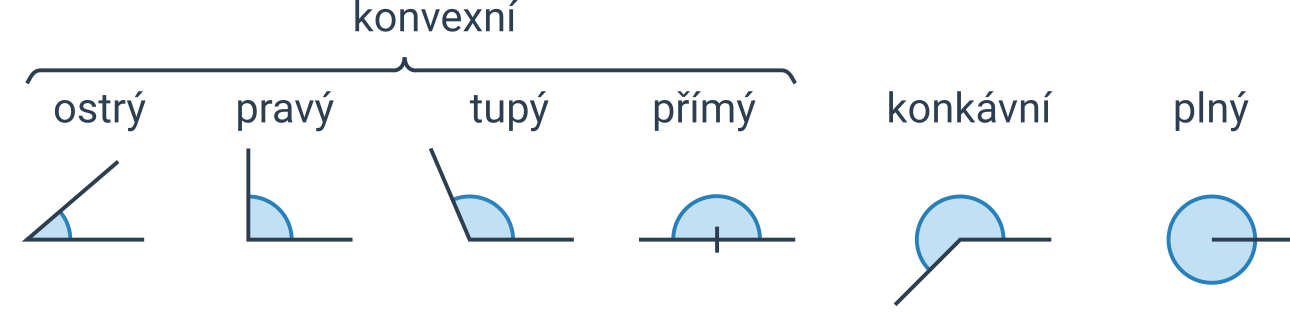
\includegraphics[width=0.8\textwidth]{uhly_dle_velikosti}
    \caption{Klasifikace úhlů podle velikosti}
  \end{figure}
\end{pozn}

\begin{definition}
  Nechť $A,B\in \mathbb E_2$. \textbf{Vzdáleností bodů} $A,B$ nazveme délku úsečky $AB.$
\end{definition}


\begin{definition}
  Nechť $P\in \mathbb E_2, p \in \mathscr P.$ \textbf{Vzdáleností bodu} $P$ \textbf{od přímky} $p$ nazveme reálné číslo označené $\rho(P,p)$ takové, že $\rho(P,p)=|PP_0|,$ kde $P_0$ je kolmý průmět bodu $P$ na přímku $p$.
\end{definition}

\begin{definition}
  Nechť $a,b \in \mathscr P, a \parallel b.$ \textbf{Vzdáleností dvou přímek} $a,b$ nazveme reálné číslo označené $\rho(a,b)$ takové, že $\rho(a,b)=\rho(A,b),$ kde $A\in a$ je libovolný bod.
\end{definition}

\begin{definition}
  Nechť $a,b\in \mathscr P.$ \textbf{Odchylkou přímek} $a,b$ nazveme reálné číslo $\varphi^\circ\in \left <0, 90\right>$, kde $\varphi$ je velikost úhlu, který spolu přímky $a,b$ svírají. U rovnoběžek klademe $\varphi = 0^\circ.$
\end{definition}

\begin{definition}
  Dva úhly nazveme
  \begin{itemize}
    \item \textbf{vrcholové}, jestliže jsou jejich ramena opačné polopřímky,
    \item \textbf{vedlejší}, jestliže je jejich jedno rameno společné a zbylá dvě ramena jsou opačné polopřímky,
    \item \textbf{souhlasné}, jestliže jejich první ramena leží na jedné přímce a druhá ramena jsou rovnoběžná, přitom směr příslušných ramen je stejný,
    \item \textbf{střídavé}, jestliže jejich první ramena leží na jedné přímce a druhá ramena jsou rovnoběžná, přitom směr příslušných ramen je opačný,
    \item \textbf{přilehlé}, jestliže jejich první ramena leží na jedné přímce a jdou do opačných směrů a~druhá ramena jsou rovnoběžná.
  \end{itemize}
  \begin{figure}[h!]
    \centering
    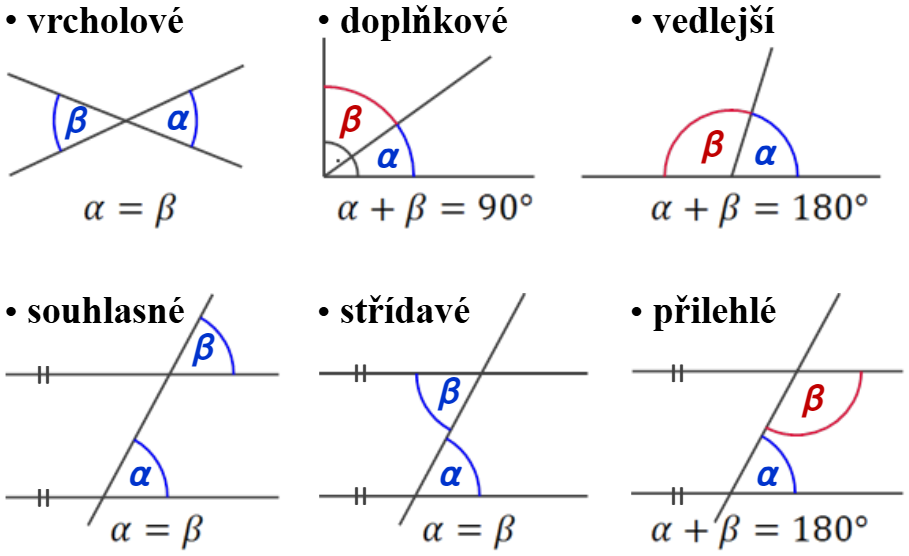
\includegraphics[width=0.5\linewidth]{dvojice_uhlu.png}
    \caption{Dvojice úhlů}
  \end{figure}
\end{definition}


\begin{definition}
  Dvě polopřímky ležící na téže přímce nazýváme \textbf{souhlasnými}, jestliže jedna z nich je podmnožinou druhé. V opačném případě je nazveme \textbf{nesouhlasnými}.
\end{definition}

\begin{definition}
  Nechť je dán trojúhelník $\triangle ABC$. \textbf{Vnitřním úhlem} $\triangle ABC$ při vrcholu $A$~(resp. $B$, resp. $C$)
  nazýváme úhly $\sphericalangle CAB$ (resp. $\sphericalangle ABC$, resp. $ \sphericalangle BCA$), \textbf{vnějším úhlem}
  $\triangle ABC$ při vrcholu $A$ (resp. $B$, resp. $C$) pak vedlejší úhel k úhlu $\sphericalangle CAB$ (resp. $\sphericalangle ABC$, resp. $\sphericalangle BCA$).
  \begin{figure}[ht!]
    \centering
    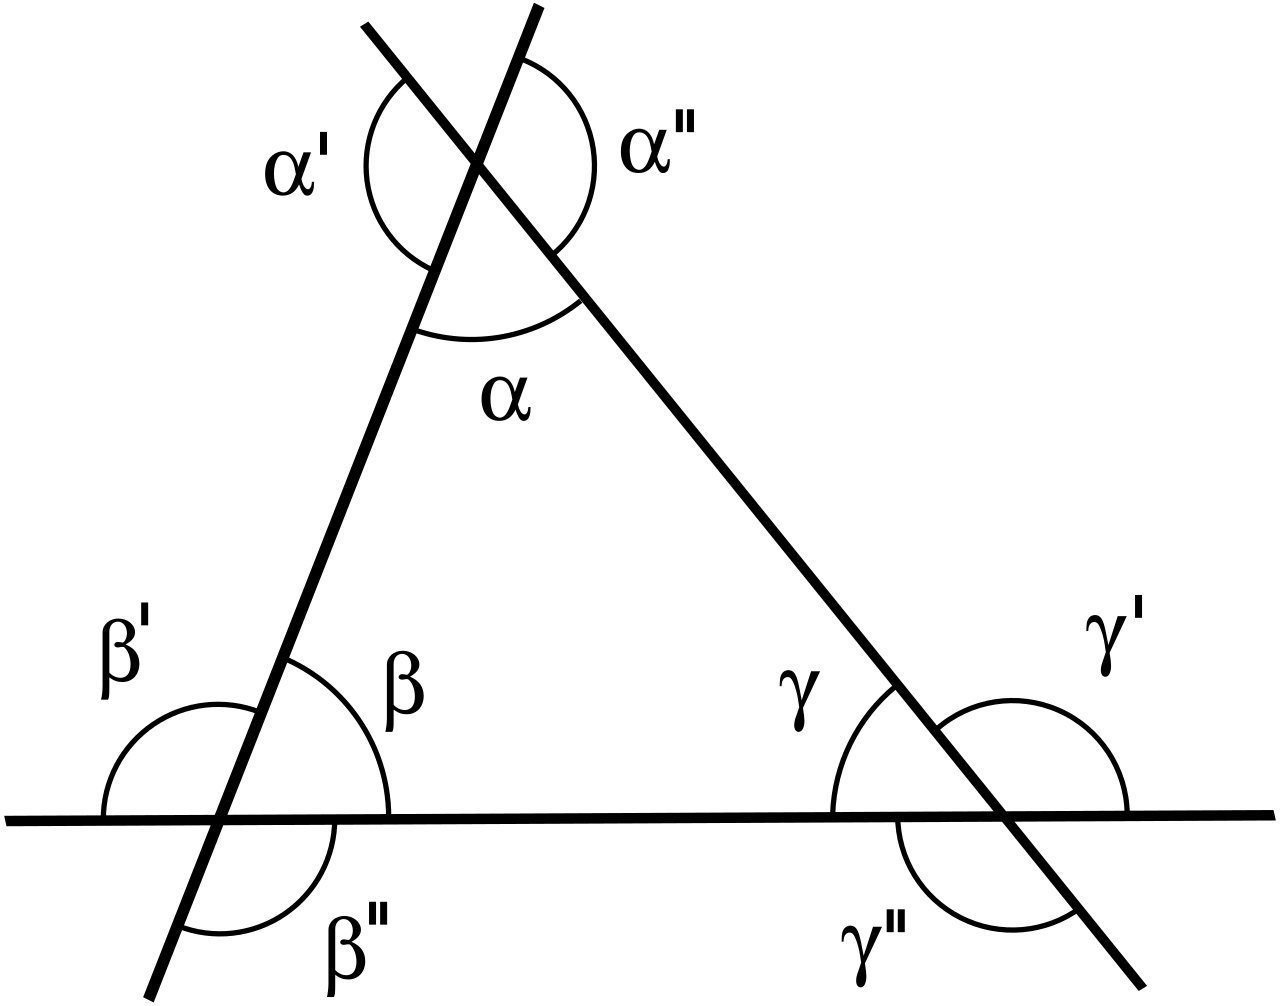
\includegraphics[width=0.3\textwidth]{trojuhelnik_uhly}
    \caption{Trojúhelník s vnitřními ($\alpha$, $\beta$, $\gamma$) a
    vnějšími ($\alpha^\prime$, $\beta ^\prime$, $\gamma^\prime$) úhly}
    \label{}
  \end{figure}
\end{definition}

\begin{veta}
  Součet všech vnitřních úhlů v trojúhelníku je $180^\circ$.
\end{veta}

\begin{proof}
    Bez újmy na obecnosti veďme bodem $A$ rovnobežku se stranou $a$.
    Odtud lze jasně vidět, že zbylé dva úhly k úhlu $\alpha$ jsou střídavé s
    úhly $\beta$, $\gamma$, a tedy i shodné. Celkem dávají přímý úhel,
    t.j. jejich součet je $180^\circ$, což jsme chtěli dokázat.
    \begin{figure}[ht!]
      \centering
      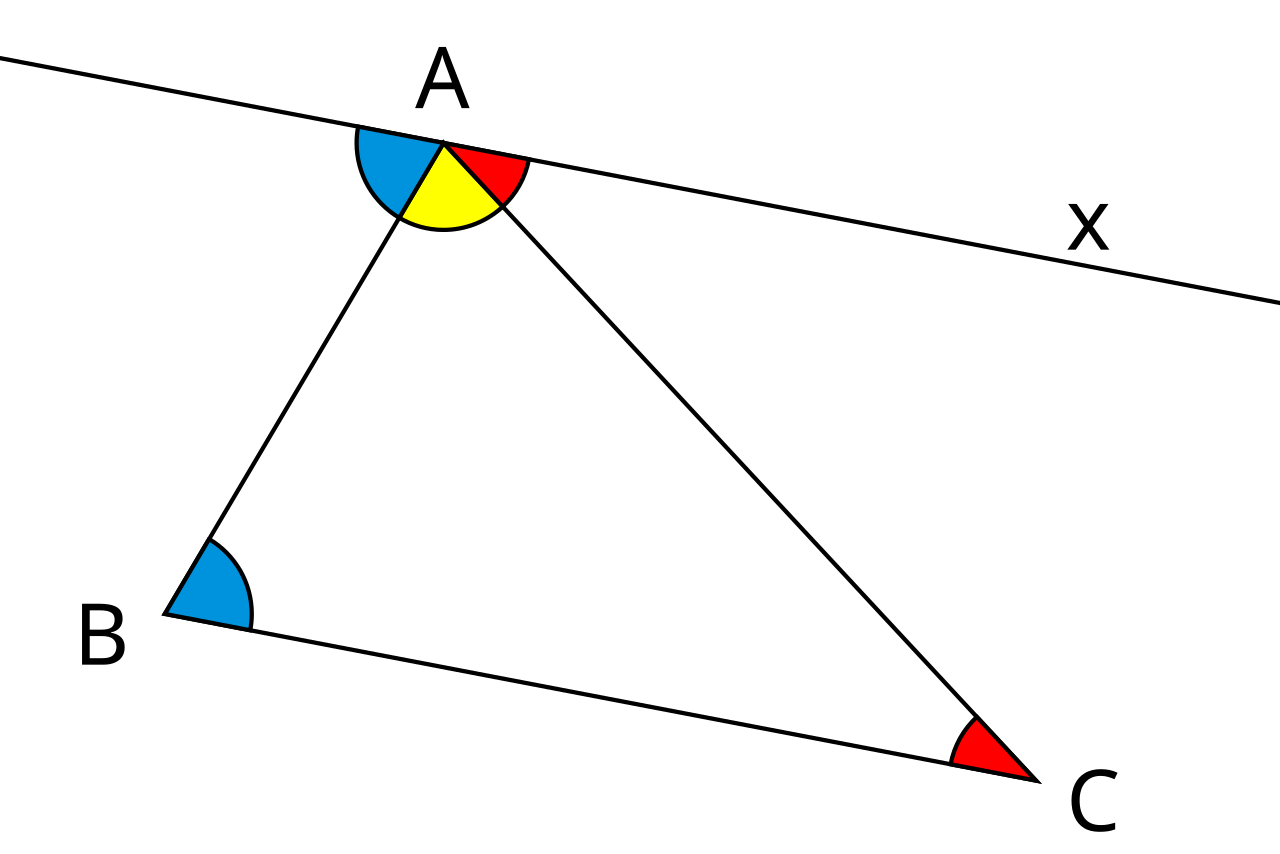
\includegraphics[width=0.3\linewidth]{soucet_uhlu_v_troj.png}
      \caption{Součet úhlů v trojúhelníku}
    \end{figure}
\end{proof}


\begin{veta}
  Součet libovolných dvou vnitřních úhlů v trojúhelníku je menší něž $180^\circ$.
\end{veta}

\begin{proof}
  Plyne z předchozí věty a tvrzení, že vnitřní úhel v trojúhelníku je nenulový.
\end{proof}

\begin{veta}
  V každém trojúhelníku je velikost vnějšího úhlu při jednom vrcholu rovna součtu velikostí dvou zbylých vnitřních úhlů.
\end{veta}

\begin{proof}
  Jistě platí $\alpha + \alpha^\prime = 180^\circ$, protože jsou to úhly
  vedlejší. Zároveň platí $\alpha + \beta + \gamma = 180^\circ$. Celkem
  tedy máme $\alpha^\prime = \beta + \gamma$, což jsme chtěli dokázat.
\end{proof}

\begin{definition}
  Trojúhelník se nazývá \textbf{rovnoramenný}, jestliže alespoň dvě jeho strany jsou shodné úsečky. Strany stejné délky nazveme \textbf{rameny}, tu třetí \textbf{základnou} a vrchol proti základně \textbf{vrcholem}.
  Trojúhelník se nazývá \textbf{rovnostranný}, jestliže všechny tři jeho strany jsou shodné úsečky.
  Trojúhelník se nazývá \textbf{pravoúhlý}, jestliže je jeden jeho vnitřní úhel pravý. Dvě strany, které jsou rameny pravého úhlu nazveme \textbf{odvěsnami}, tu třetí \textbf{přeponou}.
\end{definition}

\begin{definition}
  \textbf{Střední příčkou} trojúhelníku nazýváme úsečku spojující středy dvou stran trojúhelníka.
  \textbf{Těžnicí} trojúhelníku nazýváme úsečku spojující vrchol trojúhelníku se středem protější strany.
  \textbf{Výškou} trojúhelníku nazýváme úsečku procházející vrcholem trojúhelníka, která je kolmá na přímku, na které leží protější strana trojúhelníku. Průsečík výšek nazýváme \textbf{ortocentrum}.
\end{definition}

\begin{veta}
  Každá střední příčka je rovnoběžná s protilehlou stranou a je dvakrát menší než protilehlá strana.
\end{veta}

\begin{proof}
  Trojúhelníky vrchol -- střední příčka a vrchol -- protilehlá strana jsou zjevně podobné s koeficientem 2.
\end{proof}

\begin{veta}
  Těžnice trojúhelníka se protínají v jednom bodě, který je dělí v poměru $2:1$.
\end{veta}

\begin{proof}
    V trojúhelníku $ABC$ jsou těžnice $t_a,t_b,t_c$. Sestrojme body $X,Y$ tak, aby
    $ABXC$ a~$ABCY$ byly rovnoběžníky. Jistě jsou $AX$, resp. $BY$ jejich úhlopříčky.
    Zároveň je $|AB|=|CX|=|CY|$, takže $C$ je střed $XY$. Těžnice $t_c$ je tím pádem
    osou souměrnosti lichoběžníka $ABXY$, a~proto leží na průsečíku jeho úhlopříček
    (tento lichoběžník je rovnoramenný).\\
    V~témže trojúhelníku označme středy stran $S_a,S_b,S_c$. Trojúhelník $S_aS_bS_c$ je
    pak podobný s~trojúhelníkem $ABC$ s~koeficientem $1/2$ (jeho strany jsou středními
    příčkami trojúhelníka $ABC$). Navíc těžnice \uv{menšího} trojúhelníka leží na
    těžnicích toho \uv{většího}. Proto i~$|AT|=2|S_{S_bS_c}T|$, což jsme chtěli ukázat.
\end{proof}

\begin{definition}
Průsečík těžnic nazýváme \textbf{těžištěm}.
\end{definition}

\begin{veta}
  Nechť $\triangle ABC$ je rovnoramenný trojúhelník se základnou $AB$. Pak platí, že těžnice $t_c$ splývá s výškou $v_c$ a s osou úhlu $\sphericalangle ACB$.
\end{veta}

\begin{proof}
  Nechť $t_c = CC_1$, kde $C_1$ je středem $AB$.
  $\triangle AC_1 C \cong \triangle BC_1 C$ (sus), neboť $|AC| = |BC|, |AC_1| = |BC_1|$ a $|\sphericalangle CAC_1| = |\sphericalangle CBC_1|$
  \begin{enumerate}[$i.$]
    \item $|\sphericalangle AC_1 C| = |\sphericalangle BC_1 C| = 90^\circ \implies CC_1 = v_c$,
    \item $|\sphericalangle AC_1 C| = |\sphericalangle BC_1 C| \implies CC_1 = $ osa úhlu $\sphericalangle ACB$.\qedhere
  \end{enumerate}
\end{proof}

\begin{veta}[Trojúhelníková nerovnost]
  V každém $\triangle ABC$ platí, že součet délek dvou libovolných stran je větší než strana třetí.
\end{veta}

\begin{proof}
  Ukážeme, že $|AC| < |AB| + |BC|$. Sestrojme na $\overrightarrow{AB}$ bod $D$ tak, že $|BD| = |BC| \land B\, \mu\, AD$. $\triangle BCD$ je rovnoramenný s hlavním vrcholem B $\implies \omega_1 = \delta$
  $B\, \mu\, AD \implies \omega_1 < \omega$
  $\implies \delta < \omega \implies |AC| < |AD| = |AB| + |BD| = |AB| + |BC| \implies |AC| < |AB| + |BC|$.
\end{proof}

\begin{veta}[Věty o shodnosti trojúhelníků]
  \,

  \begin{itemize}
    \item \textbf{sss}: Shodují-li se dva trojúhelníky ve všech třech odpovídajících si stranách, jsou shodné.
    \item \textbf{sus}: Shodují-li se dva trojúhelníky ve dvou stranách a úhlu jimi sevřeném, jsou shodné.
    \item \textbf{usu}: Shodují-li se dva trojúhelníky v jedné straně a v obou úhlech k ní přilehlých, jsou shodné.
    \item \textbf{Ssu}: Shodují-li se dva trojúhelníky ve dvou stranách a úhlu proti delší z nich, jsou shodné.
  \end{itemize}
\end{veta}

\begin{proof}
  Jednu si určíme jako axiom (třeba sus) a zbylé převedeme na tuto rozkladem na případy.
\end{proof}

\begin{definition}
  Trojúhelníky jsou \textbf{podobné}, zapisujeme $\triangle ABC \approx \triangle DEF$, jestliže $\exists k \in \R^+:k = \frac{|AB|}{|DE|}=\frac{|BC|}{|EF|}=\frac{|CA|}{|FD|}$. Číslo $k$ nazveme \textbf{koeficientem podobnosti}.
\end{definition}

\begin{veta}[Věty o podobnosti trojúhelníků]
  \,
  \begin{itemize}
    \item \textbf{uu}: Shodují-li se dva trojúhelníky ve dvou úhlech, jsou podobné.
    \item \textbf{sus}: Shodují-li se dva trojúhelníky v poměru dvou stran a úhlu jimi sevřeném, jsou podobné.
  \end{itemize}
\end{veta}

\begin{veta}[Euklidova věta o výšce]
  Nechť je dán pravoúhlý trojúhelník ABC s přeponou AB. Pak
  $$v_c^2 = c_a \cdot c_b$$
  \begin{figure}[ht!]
    \centering
    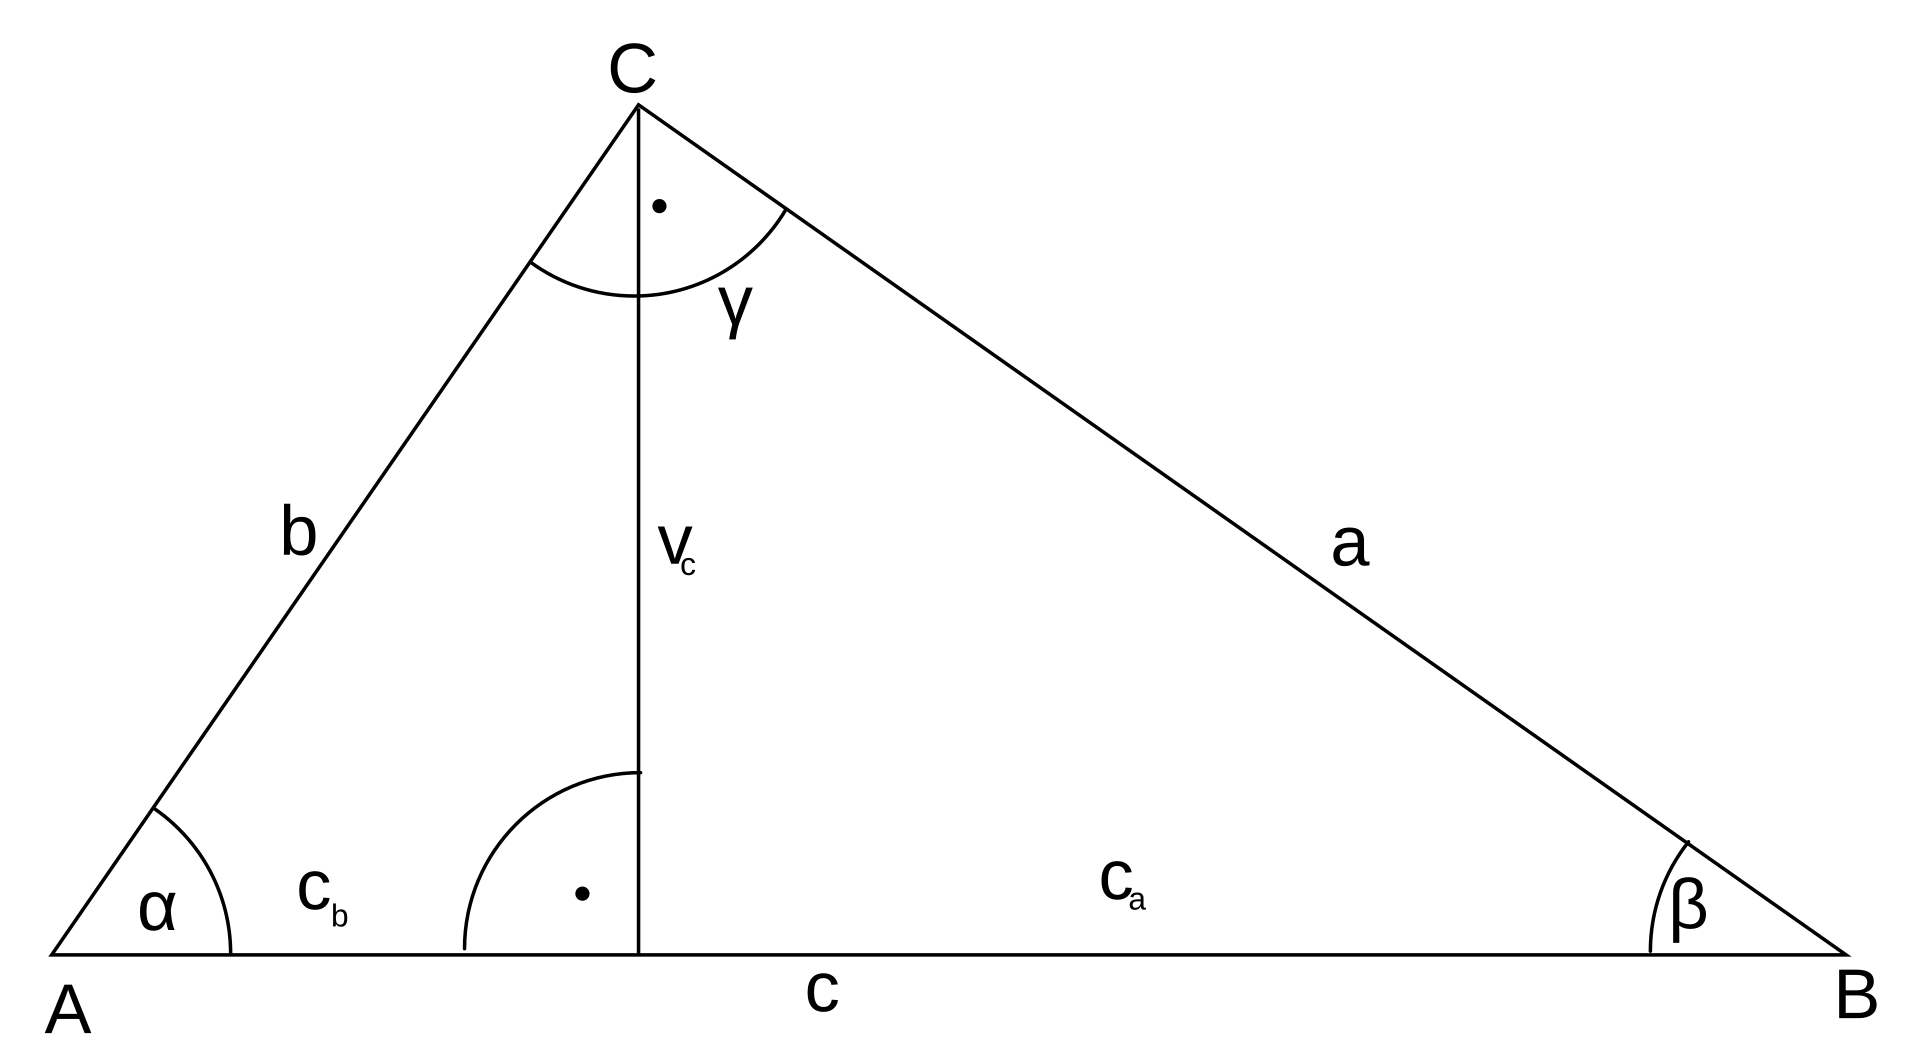
\includegraphics[width=0.4\textwidth]{eukl_v_o_vysce}
    \caption{Euklidova věta o výšce}
    \label{eukl_v_o_v}
  \end{figure}
\end{veta}

\begin{proof}
  Podle obrázku \ref{eukl_v_o_v} je $\triangle ACC_0 \approx \triangle CBC_0$, kde $C_0$ je kolmý průmět bodu $C$ na stranu $AB$ (dle věty uu), neboť $\sphericalangle C_0 CB$ je otočením $\sphericalangle C_0 AC$. Pak taky $\frac{|CC_0|}{|AC_0|} = \frac{|BC_0|}{|CC_0|} \implies \frac{v_c}{c_b} = \frac{c_a}{v_c}$ a tedy $v_c^2 = c_a \cdot c_b$, což jsme chtěli dokázat.
\end{proof}

\begin{veta}[Euklidovy věty o odvěsnách]
  Nechť je dán pravoúhlý trojúhelník s přeponou AB. Pak
  \begin{align*}
    b^2 = c \cdot c_b\\
    a^2 = c \cdot c_a
  \end{align*}
\end{veta}

\begin{proof}
  Podle obrázku \ref{eukl_v_o_v} je
  $\triangle ABC \approx \triangle CBC_0$, kde $C_0$ je kolmý průmět bodu $C$ na stranu $AB$ (dle věty uu), neboť $\sphericalangle C_0 BC$ je otočením $\sphericalangle CBA$. Pak taky $\frac{|BC_0|}{|BC|} = \frac{|BC|}{|AB|} \implies \frac{c_a}{a} = \frac{a}{c}$ a~tedy $a^2 = c_a \cdot c$, což jsme chtěli dokázat.
\end{proof}

\begin{veta}[Pythagorova]
  Nechť je dán pravoúhlý trojúhelník $ABC$ s přeponou $c$. Pak
  \[
    a^2+b^2 = c^2.
  \]
\end{veta}


\begin{proof}
  Z Euklidovy věty o výšce platí $cc_a=a^2$, $cc_b=b^2$, po sečtení těchto dvou vztahů získáme
  \[
    cc_a+cc_b=a^2+b^2 \iff c(c_a+c_b)=a^2+b^2 \iff c^2=a^2+b^2. \qedhere
  \]
\end{proof}

\begin{definition}
  Nechť $A_1,A_2, A_3, A_4 \in \mathbb E_2$ jsou čtyři body, z nichž žádné tři nejsou kolineární. Sjednocení úseček $A_1A_2\cup A_2A_3 \cup A_3A_4 \cup A_4A_1$ nazveme \textbf{uzavřenou lomenou čárou}.
\end{definition}

\begin{definition}
  Nechť $ABCD$ je uzavřená lomená čára, která sama sebe neprotíná. Pak \textbf{čtyřúhelníkem} $ABCD$ nazveme sjednocení této lomené čáry s množinou jejích vnitřních bodů. Body $A,B,C,D$ se nazývají \textbf{vrcholy}, uzavřená lomená čára $ABCD$ \textbf{obvodem}, každá úsečka \textbf{stranou} a úsečky $AC,BD$ se nazývají \textbf{úhlopříčky}.
\end{definition}

\begin{veta}
  Součet vnitřních úhlů čtyřúhelníka je $360^\circ$.
\end{veta}

\begin{proof}
  Čtyřúhelník $ABCD$ lze rozdělit na dva trojúhelníky
  $\triangle ABD $ a $\triangle BCD$ jako na obrázku.
  Pak jistě platí $\alpha + \beta_1 + \delta_1 = 180^\circ$ a
  $\beta_2 + \gamma + \delta_2 = 180^\circ$. Součet všech vnitřních úhlů
  čtyřúhelníka $ABCD$ je tedy $\alpha + \beta_1 + \beta_2 + \gamma + \delta_1
  + \delta_2 = 360^\circ$, což jsme chtěli dokázat.
  \begin{figure}[ht!]
    \centering
    \scalebox{0.6}{\tikzfig{figures/ctyruhelnik}}
    \caption{Čtyřúhelník $ABCD$}
  \end{figure}
\end{proof}

\begin{definition}
  Nechť $ABCD$ je čtyřúhelník, jehož protější strany jsou rovnoběžné. Pak ho nazveme \textbf{rovnoběžníkem}.
\end{definition}

\begin{veta}
  V rovnoběžníku $ABCD$ platí:
  \begin{enumerate}[$i.$]
    \item $|AB|=|CD| \land |BC|=|AD|,$
    \item protilehlé úhly jsou shodné.
  \end{enumerate}
\end{veta}

\begin{proof}
  Plyne ze shodnosti trojúhelníků $\triangle ABD$ a $\triangle CDB.$
\end{proof}

\begin{veta}
  Úhlopříčky rovnoběžníka se navzájem půlí.
\end{veta}


\begin{proof}
  Plyne ze shodnosti trojúhelníků $\triangle ASD$ a $\triangle CSB$, kde $S$ je průsečík úhlopříček.
\end{proof}

\begin{definition}
  Čtyřúhelník, jehož všechny čtyři úhly jsou pravé, nazveme \textbf{pravoúhelník}.
\end{definition}

\begin{veta}\,
  \begin{enumerate}[$i.$]
    \item Každý pravoúhelník je rovnoběžník.
    \item Úhlopříčky pravoúhelníka jsou shodné.
  \end{enumerate}
\end{veta}

\begin{proof}\,
  \begin{enumerate}[$i.$]
    \item Protější úhly v rovnoběžníku jsou střídavé úhly u rovnoběžek.
    \item Plyne ze shodnosti trojúhelníků $ABD$ a $BAC$.\qedhere
  \end{enumerate}
\end{proof}

\begin{definition}
  Rovnoběžník $ABCD$ se nazývá \textbf{kosočtvercem} (resp. \textbf{kosodélníkem}), jestliže $|AB|=|BC|$ (resp. $|AB| \neq |BC|$) a žádný vnitřní úhel není pravý.
\end{definition}


\begin{veta}
  Úhlopříčky v kosočtverci se navzájem půlí.
\end{veta}

\begin{definition}
  Pravoúhelník $ABCD$ nazýváme
  \begin{itemize}
    \item \textbf{čtvercem}, jestliže $|AB|=|BC|,$
    \item \textbf{obdélníkem}, jestliže $|AB| \ne |BC|$.
  \end{itemize}
\end{definition}

\begin{definition}
  Konvexní čtyřúhelník $ABCD$, kde $AB \parallel CD \land BC \nparallel AD,$ nazveme \textbf{lichoběžníkem}. Strany $AB, CD$ nazveme \textbf{základnami} a strany $BC$ a $DA$ \textbf{rameny lichoběžníka}.
\end{definition}

\begin{definition}
  Uzavřená lomená čára $A_1A_2\dots A_nA_1$, která leží v rovině a sama sebe nikdy neprotíná ohraničuje část roviny, která se nazývá \textbf{mnohoúhelník} nebo také \textbf{$n$-úhelník}.
\end{definition}

\begin{definition}
  Nechť $S \in \mathbb E_2, r \in \mathbb R^+.$  \textbf{Kružnicí} (resp. \textbf{kruhem}) se středem $S$ a poloměrem $r$ nazýváme množinu všech bodů $X\in \mathbb E_2, $ kde $|SX|=r$ (resp. $|SX|\leq r$).
\end{definition}

\begin{definition}
  Nechť $k(S,r)$ je kružnice, $X_1, X_2 \in k, X_1\ne X_2.$ Úsečku (resp. přímku) $X_1X_2$ nazýváme \textbf{tětivou} (resp. \textbf{sečnou}) kružnice $k$.
\end{definition}


\begin{definition}
  Nechť $k(S,r)$ je kružnice, $T\in k$. Přímku $t$, pro níž platí $T\in t \land ST \perp t$ nazýváme \textbf{tečnou} kružnice $k$ s \textbf{bodem dotyku} $T$.
\end{definition}

\begin{definition}
  Nechť je dán oblouk $AB$ na kružnici $k(S,r).$ Polopřímky $\overrightarrow{SA}, \overrightarrow{SB}$ jsou rameny dvou úhlů,
  z nichž právě jedno obsahuje oblouk $AB$. Tento úhel nazýváme \textbf{středovým úhlem} příslušným oblouku $AB$.
  Každý úhel $\sphericalangle AXB,$ kde $X\in k \land X\notin AB,$ nazýváme \textbf{obvodovým úhlem} příslušným oblouku $AB$.
\end{definition}

\begin{veta}
  Nechť $k(S,r)$ je kružnice. Pak středový úhel je dvojnásobkem libovolného obvodového úhlu příslušného k témuž oblouku kružnice.
\end{veta}

\begin{proof}
  Rozdělíme na tři případy polohy ostrého obvodového úhlu $\sphericalangle AXB$ vůči středu kružnice $S$.
  \begin{enumerate}[$i.$]
    \item střed kružnice leží na rameni obvodového úhlu\\
    Trojúhelník $\triangle SXB$ je rovnoramenný se základnou $BX$, takže $|\sphericalangle SBX| = |\sphericalangle SXB|=\varphi$. Označme $|\sphericalangle ASB|=\omega$. Pak $2\varphi + (180^\circ - \omega)=180^\circ$, tedy $\omega = 2\varphi$, což jsme chtěli dokázat.
    \item střed kružnice leží uvnitř obvodového úhlu\\
    Označme průsečík přímky $XS$ s kružnicí $k$, který je různý od $X$ jako $C$. Pak protože $|\sphericalangle AXC|=2\cdot|\sphericalangle ASC|$ a
    $|\sphericalangle BXC|=2\cdot|\sphericalangle BSC|$, což už jsme dokázali v $i.$, pak i~$|\sphericalangle AXB| = 2\cdot|\sphericalangle ASB|$.
    \item střed kružnice leží vně obvodového úhlu\\
    Označme průsečík přímky $XS$ s kružnicí $k$, který je různý od $X$ jako $C$. Pak $|\sphericalangle BXC| = 2\cdot|\sphericalangle BSC|$ a $|\sphericalangle AXC|=2\cdot|\sphericalangle ASC|$, což už jsme dokázali v $i.$. Pak i $|\sphericalangle AXB| = 2\cdot|\sphericalangle ASB|$.\qedhere
  \end{enumerate}
\end{proof}

\begin{veta}
  Každé dva obloukové úhly příslušné témuž oblouku kružnice jsou shodné.
\end{veta}

\begin{veta}[Thaletova]
  Každý obvodový úhel příslušný polokružnici je pravý.
\end{veta}

\begin{figure}[ht!]
  \centering
  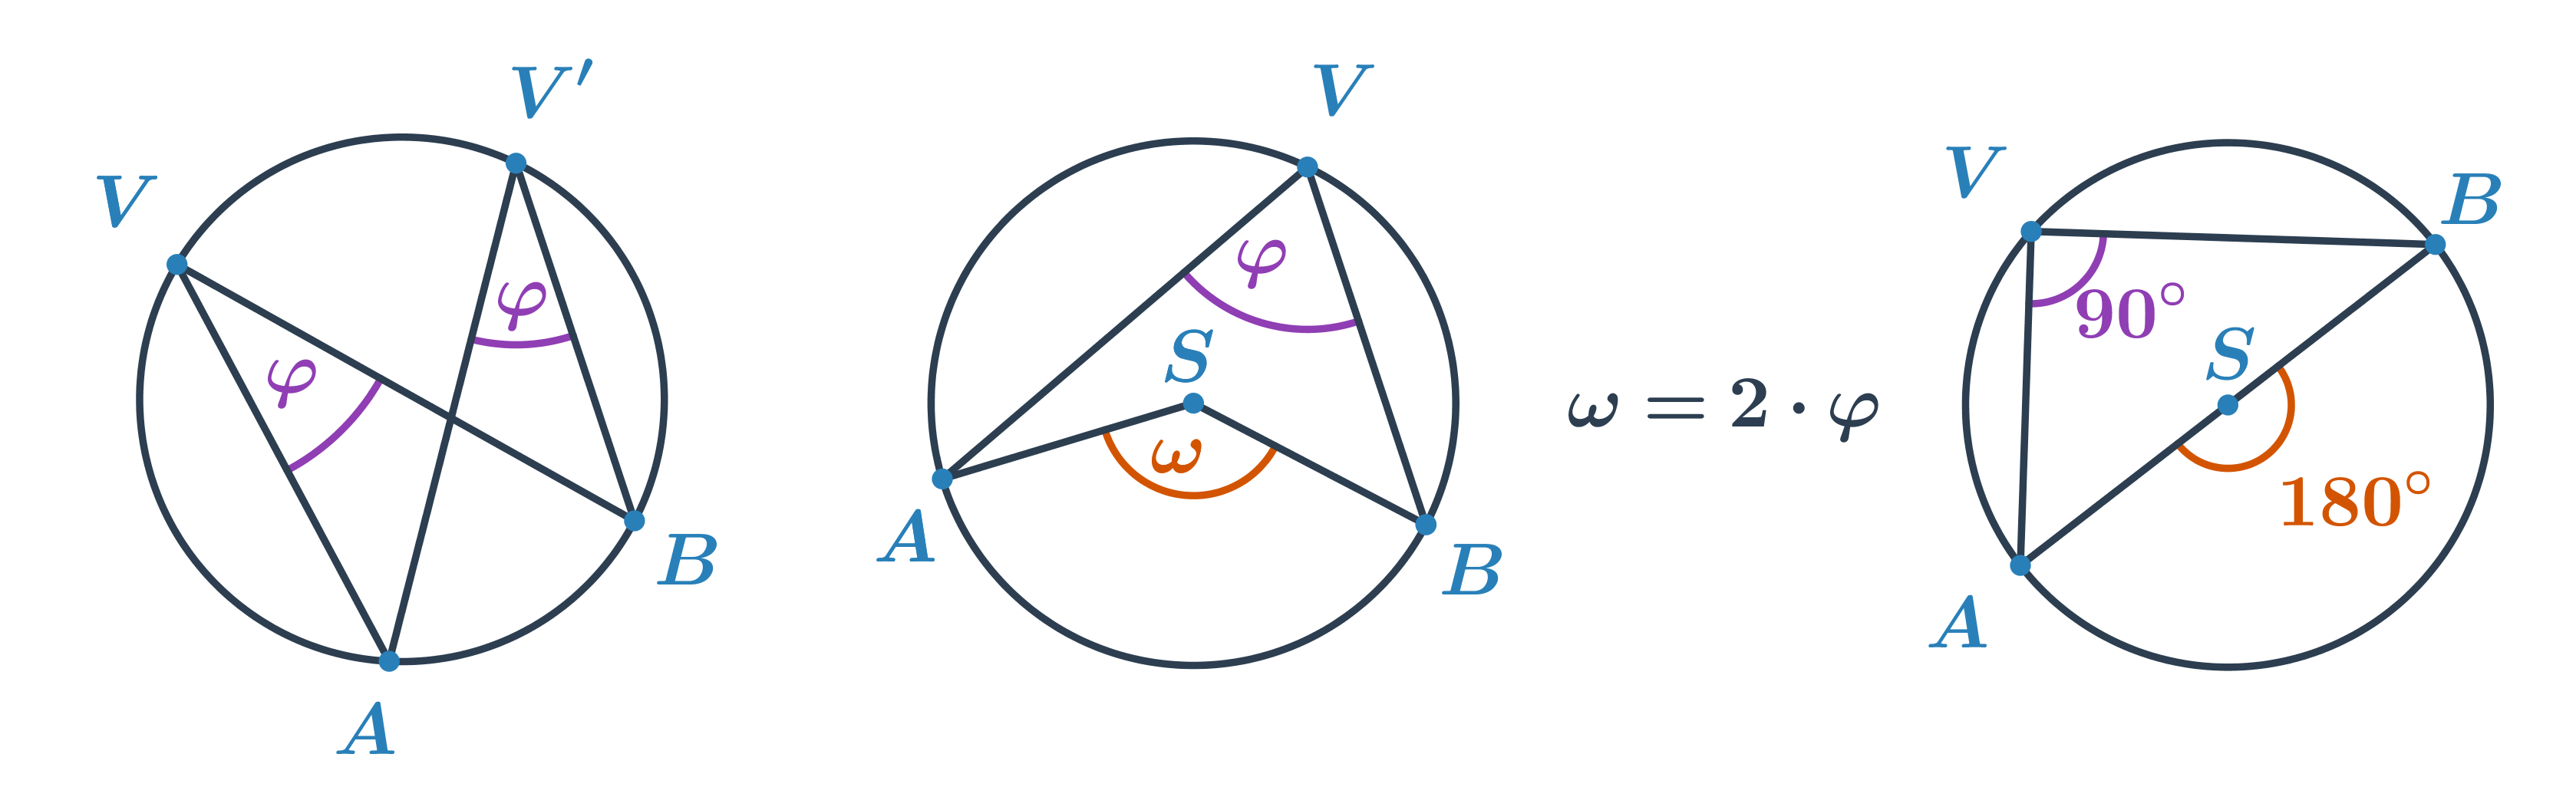
\includegraphics[width=0.7  \textwidth]{obvodovy_uhel}
  \caption{Obvodový a středový úhel, Thaletova kružnice}
\end{figure}

\begin{definition}
  Nechť $AB$ je menší oblouk kružnice $k(S,r)$, $t$ tečna ke kružnici $k$ v bodě $A$, bod $C\in t$, $C\in o$, kde $o$ je polorovina k $\overrightarrow{ABS}.$ Úhel $\sphericalangle CAB$ nazýváme \textbf{úsekovým úhlem} příslušným oblouku $AB$.
\end{definition}

\begin{veta}
  Úsekový úhel příslušný oblouku $AB$ má stejnou velikost jako obvodový úhel příslušný témuž oblouku.
\end{veta}

\begin{figure}[ht!]
  \centering
  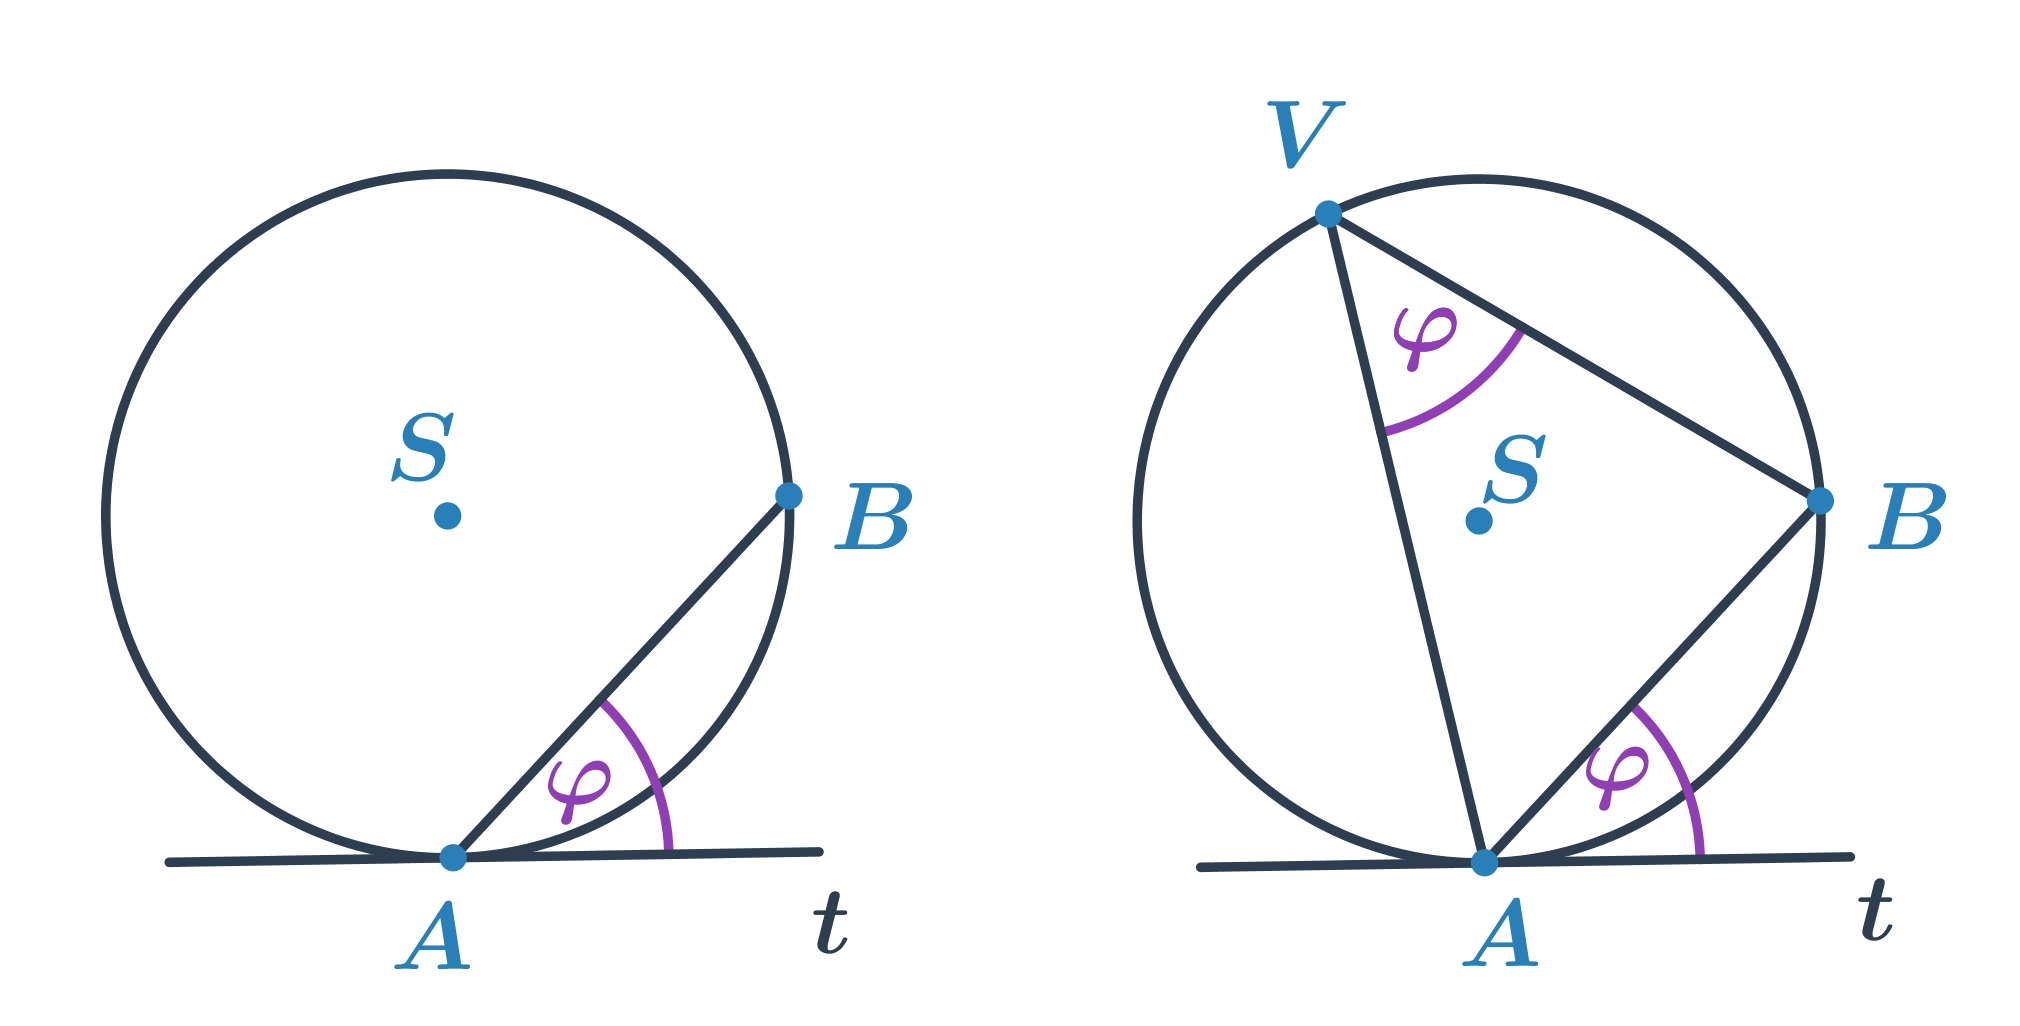
\includegraphics[width=0.45\textwidth]{usekovy}
  \caption{Úsekový úhel}
\end{figure}

\begin{definition}
  Nechť $AB$ je úsečka. \textbf{Osou úsečky} $AB$ nezveme přímku $o$, která prochází středem úsečky $AB$ a je na ni kolmá.
\end{definition}

\begin{veta}\label{mbdv}
  Nechť $AB$ je úsečka. Množinou všech bodů $X\in \mathbb E_2,$ pro něž $|AX|=|BX|$, je \textbf{osa} $o$ \textbf{úsečky} $AB$.
\end{veta}

\begin{proof}
  Označme $U=\{ X\in \mathbb E_2: |AX|=|BX| \}$.
  \begin{enumerate}[$i.$]
    \item $o \subseteq U: X \in o$ lib. $\implies$ nechť $X\in AB \implies X=S$ -- střed $AB \implies |AS|=|BS| \implies X \in U.$ Nechť $X \notin AB \implies \triangle ASX \cong \triangle BSX$ (sus) $\implies |AX|=|BX| \implies X \in U$.
    \item $U \subseteq o: X \in U$ lib. $\implies |AX|=|BX| \implies$ nechť $X \in AB \implies X=S \in o.$ Nechť $X \notin AB \implies \exists \triangle ABC$ -- rovnoramenný se základnou $AB$, kde $XS$ je těžnice, ale i~výška $\implies XS \perp AB \implies X \in o.$ \qedhere
  \end{enumerate}
\end{proof}

\begin{veta}
  Nechť $AB$ je úsečka, $o$ její osa. Pak platí:
  \begin{enumerate}[$i.$]
    \item $\overrightarrow{oA}=\{ X\in \mathbb E_2:|AX|\leq |BX| \},$
    \item $\overrightarrow{oB}=\{ X \in \mathbb E_2 : |AX| \geq |BX| \}.$
  \end{enumerate}
\end{veta}

\begin{proof}\,
  \begin{enumerate}[$i.$]
    \item Nechť $X\in \overrightarrow{oA}$. Nechť $X\in o\implies$ platí podle věty \ref{mbdv}. Nechť $X\notin o$. Nechť $X\in AB$ -- zřejmé. Nechť $X\notin AB$. Označme $Y\in o \cap BX$, $|BX|=|BY|+|YX|=|AY|+|YX|>|AX|\implies |BX|>|AX|\implies$ platí vlastnost.
    \item Nechť $X\notin \overrightarrow{oA}$. Nechť $X\notin o \implies X\in \overrightarrow{oB}\implies |BX|<|AX|\implies$ neplatí vlastnost pro polorovinu $\overrightarrow{oA}.$ \qedhere
\end{enumerate}
\end{proof}

\begin{veta}
  Nechť $a,b$ jsou dvě různoběžky, $a\cap b = \{P\}.$ Množinou všech bodů $X\in \mathbb E_2$, pro něž platí $\rho(X,a)=\rho(X,b)$, je sjednocení přímek $o_1\cap o_2,$ kde  $o_1$, $o_2$ jsou osy úhlů, které přímky $a,b$ svírají.
\end{veta}


\begin{definition}
  Nechť $a,b$ jsou dvě různé rovnoběžky. Množinou všech bodů $X\in \mathbb E_2,$ pro něž platí $\rho(X,a)=\rho(X,b)$ je přímka $o\parallel a$, kde $\rho(o,a)=\rho(o,b)$. Tuto přímku nazveme \textbf{osou pásu} s hraničními přímkami $a,b$.
\end{definition}

\begin{veta}
  Nechť $\sphericalangle AVB$ je konvexní nenulový úhel. Množinou všech bodů $X\in \mathbb E_2, X\in \sphericalangle AVB,$ pro něž platí $\rho(X, \overrightarrow{VA})=\rho(X,\overrightarrow{VB}),$ je polopřímka $o$, která je osou konvexního úhlu $\sphericalangle AVB.$
\end{veta}

\begin{definition}
  Nechť $p$ je přímka. Množinou všech bodů $X \in \mathbb E_2,$ které mají od přímky $p$~stejnou vzdálenost $a\in \mathbb R^+$, je sjednocení přímek $e_1\cup e_2,$ kde $e_1 \parallel e_2 \land \rho(e_1,p)=\rho(e_2,p)=a$. Tyto přímky nazveme
  \textbf{ekvidistantou přímky} $p$.
\end{definition}

\begin{definition}
  Nechť $k(S,r)$ je kružnice. Množinou všech bodů $X\in \mathbb E_2,$ které mají od kružnice $k$~stejnou vzdálenost $a, a \in \mathbb R^+, a< r,$ je sjednocení kružnic $e_1, e_2,$ kde kružnice $k,e_1,e_2$ jsou soustředné a~platí $\rho(e_1,k)= \rho(e_2,k)=a.$ Tyto kružnice nazveme
  \textbf{ekvidistantou kružnice} $k$.
\end{definition}

\begin{definition}
  Nechť $AB$ je úsečka. Množinou všech vrcholů $C\in \mathbb E_2$ všech pravoúhlých trojúhelníků $\triangle ABC$ s přeponou $AB$ je množina $k\smallsetminus\{ A,B\}$, kde $k\left (S,\frac{|AB|}{2}\right )$ je kružnice, $S$~je střed $AB$. Tuto množinu budeme nazývat \textbf{Thaletovou kružnicí} nad přeponou $AB$ a~označovat $\tau (AB).$
\end{definition}

\begin{veta}
  Nechť $AB$ je úsečka, $|\sphericalangle ACB|$ velikost úhlu $\gamma.$ Množinou vrcholů $X\in \mathbb E_2$ všech $\triangle ABX$ s jednou stranou $AB$ a úhlem $\gamma$ o velikosti $|\sphericalangle ACB|$ je sjednocení vnitřku oblouku $ACB$ s jeho obrazem $AC^\prime B^\prime$ v souměrnosti podle přímky $AB$.
\end{veta}

\begin{pozn}
  Pokud $\sphericalangle AXB = \alpha,$ pak říkáme, že úsečka $AB$ je vidět z bodu $X$ pod úhlem $\alpha$, resp. úhel $\alpha$ se nazývá \textbf{zorným úhlem úsečky} $AB.$
\end{pozn}

\begin{definition}
  Nechť $\triangle ABC$ je trojúhelník. Kružnici, která prochází body $A,B,C$, nazveme \textbf{kružnicí opsanou} trojúhelníku $\triangle ABC.$ Kružnici, která se dotýká všech tří stran trojúhelníku $\triangle ABC,$ nazveme \textbf{kružnici vepsanou} trojúhelníku $\triangle ABC.$
\end{definition}

\begin{veta}
  Střed kružnice trojúhelníku opsané (resp. vepsané) leží v průsečíku os stran (resp. os úhlů) daného trojúhelníku.
\end{veta}

\begin{definition}
  Nechť je dána kružnice $k(S,r).$ Konvexní čtyřúhelník $ABCD$, který je vepsán do kružnice $k$, nazýváme \textbf{tětivovým čtyřúhelníkem}. Konvexní čtyřúhelník $EFGH$, který je opsán kružnici $k$, nazýváme \textbf{tečnovým čtyřúhelníkem}.
\end{definition}

\begin{veta}
  Nechť je dán čtyřúhelník $ABCD$ se stranami $a,b,c,d$ a úhly $\alpha, \beta, \gamma, \delta.$ Pak platí:
  \begin{itemize}
    \item $ABCD$ je tětivový $\iff \alpha + \gamma=\beta+\delta=180^\circ,$
    \item $ABCD$ je tečnový $\iff a+c=b+d.$
  \end{itemize}
\end{veta}

\begin{definition}
  Je dán bod $M$ a kružnice $k$ se středem $O$ a poloměrem $r$. \textbf{Mocností bodu} $M$ \textbf{ke kružnici} $k$ rozumíme číslo $p(M, k) = |MO|^2-r^2.$
\end{definition}

\begin{veta}
  Nechť přímka $p$ vedená bodem $M$ protne kružnici $k$ v bodech $A,B$. Pak platí
  $$
    p(M,k)=
    \begin{cases}
      |MA|\cdot |MB|, & \text{leží-li } $M$ \text{ vně } $k$, \\
      -|MA|\cdot |MB|, & \text{leží-li } $M$ \text{ uvnitř } $k$.
    \end{cases}
  $$
\end{veta}

\begin{proof}
Nechť je dána kružnice $k(O,r)$ a bod $M$, který leží v její vnější oblasti. Bodem $M$ je dále
vedena přímka, která protne kružnici $k$ v bodech $A,B$ tak, že $B\in \overrightarrow{AM}$.
Konečně veďme bodem $M$ tečnu s bodem dotyku $T$ ke kružnici $k$ takovou, že přímka
$\overleftrightarrow{AM}$ neodděluje body $O$ a $T$.\\
Úhly $\sphericalangle MAT$ a $\sphericalangle BTM$ jsou shodné, protože jsou úhlem obvodovým, resp.
úsekovým příslušným témuž oblouku $BT$. Pak jsou trojúhelníky $\triangle ATM$ a $\triangle TBM$ podobné.
Platí tedy
$$\frac{|MB|}{|MT|}=\frac{|MT|}{|MA|} \iff |MT|^2=|MA|\cdot |MB|.$$
Jenže $MT$ je odvěsnou pravoúhlého trojúhelníka $\triangle OMT$ s přeponou $OM$. Je tedy
$$p(M,r)=|OM|^2-r^2=|MT|^2=|MA|\cdot |MB|,$$
což jsme chtěli dokázat.
Obdobně postupujeme i je-li $M$ ve vnitřní oblasti kružnice $k$.
\end{proof}


\begin{priklad}
Dvě kružnice se protínají ve dvou bodech $A,B$, bod $X \in \overleftrightarrow{AB},$
ale neleží na úsečce $AB$. Dokažte, že délky úseků na tečnách vedených z bodu $X$
ke kružnicím jsou shodné.
\end{priklad}

\begin{reseni}
Označme body dotyku $T_1,T_2.$ Z mocnosti bodu ke kružnici platí
$|T_1X|^2=|XB|\cdot |XA|=|XT_2|^2.$
\end{reseni}

\begin{priklad}
Je dána přímka $p$, kružnice $k_1, k_2$ v opačných polorovinách s hranicí $p.$
Sestrojte úsečku $XY$ tak, aby $X\in k_1, Y\in k_2, \overleftrightarrow{XY} \perp p,$ a
střed úsečky $XY$ ležel na $p.$
\end{priklad}

\begin{reseni}
Rozbor: $XY\perp p \, \land$ střed $XY\in p \implies X=\mathcal O_p(Y)$. Hledáme
bod $X$: buď $X \in k_1$, nebo $X=\mathcal O_p(Y) \, \land \, Y \in k_2 \implies X \in \mathcal O_p(k_2)=k_2^\prime,$ celkem
tedy máme $X\in k_1\cap k_2^\prime.$ Dále nesmíme v řešení zapomenout zahrnout taky postup
konstrukce, samotnou konstrukci a~diskuzi počtu řešení (tady v závislosti na
počtu průniků $k_1$ s $k_2^\prime$).
\end{reseni}

\begin{priklad}
Jsou dány dvě rovnoběžky $a,b$ a mimo ně bod $C$. Sestrojte rovnostranný
trojúhelník $ABC$ tak, aby $A \in a, B \in b$.
\end{priklad}

\begin{reseni}
Strana $AC$ je stejně dlouhá jako $BC$ a navíc svírají úhel $60^\circ$. Bod
$B$ tedy nalezneme jako průnik přímky $b$ s otočením přímky $a$ o $60^\circ$ kolem
bodu $C.$
\end{reseni}

\begin{priklad}
Zobrazte bod $X$ ve stejnolehlosti dané bodem $S$ a koeficientem
\begin{enumerate}[$i.$]
\item $\lambda = 3,$
\item $\lambda = \frac{1}{3},$
\item $\lambda = -\frac{1}{3},$
\item $\lambda = -3.$
\end{enumerate}
\end{priklad}

\begin{reseni}
Řešení vypadá následovně:
\begin{center}
 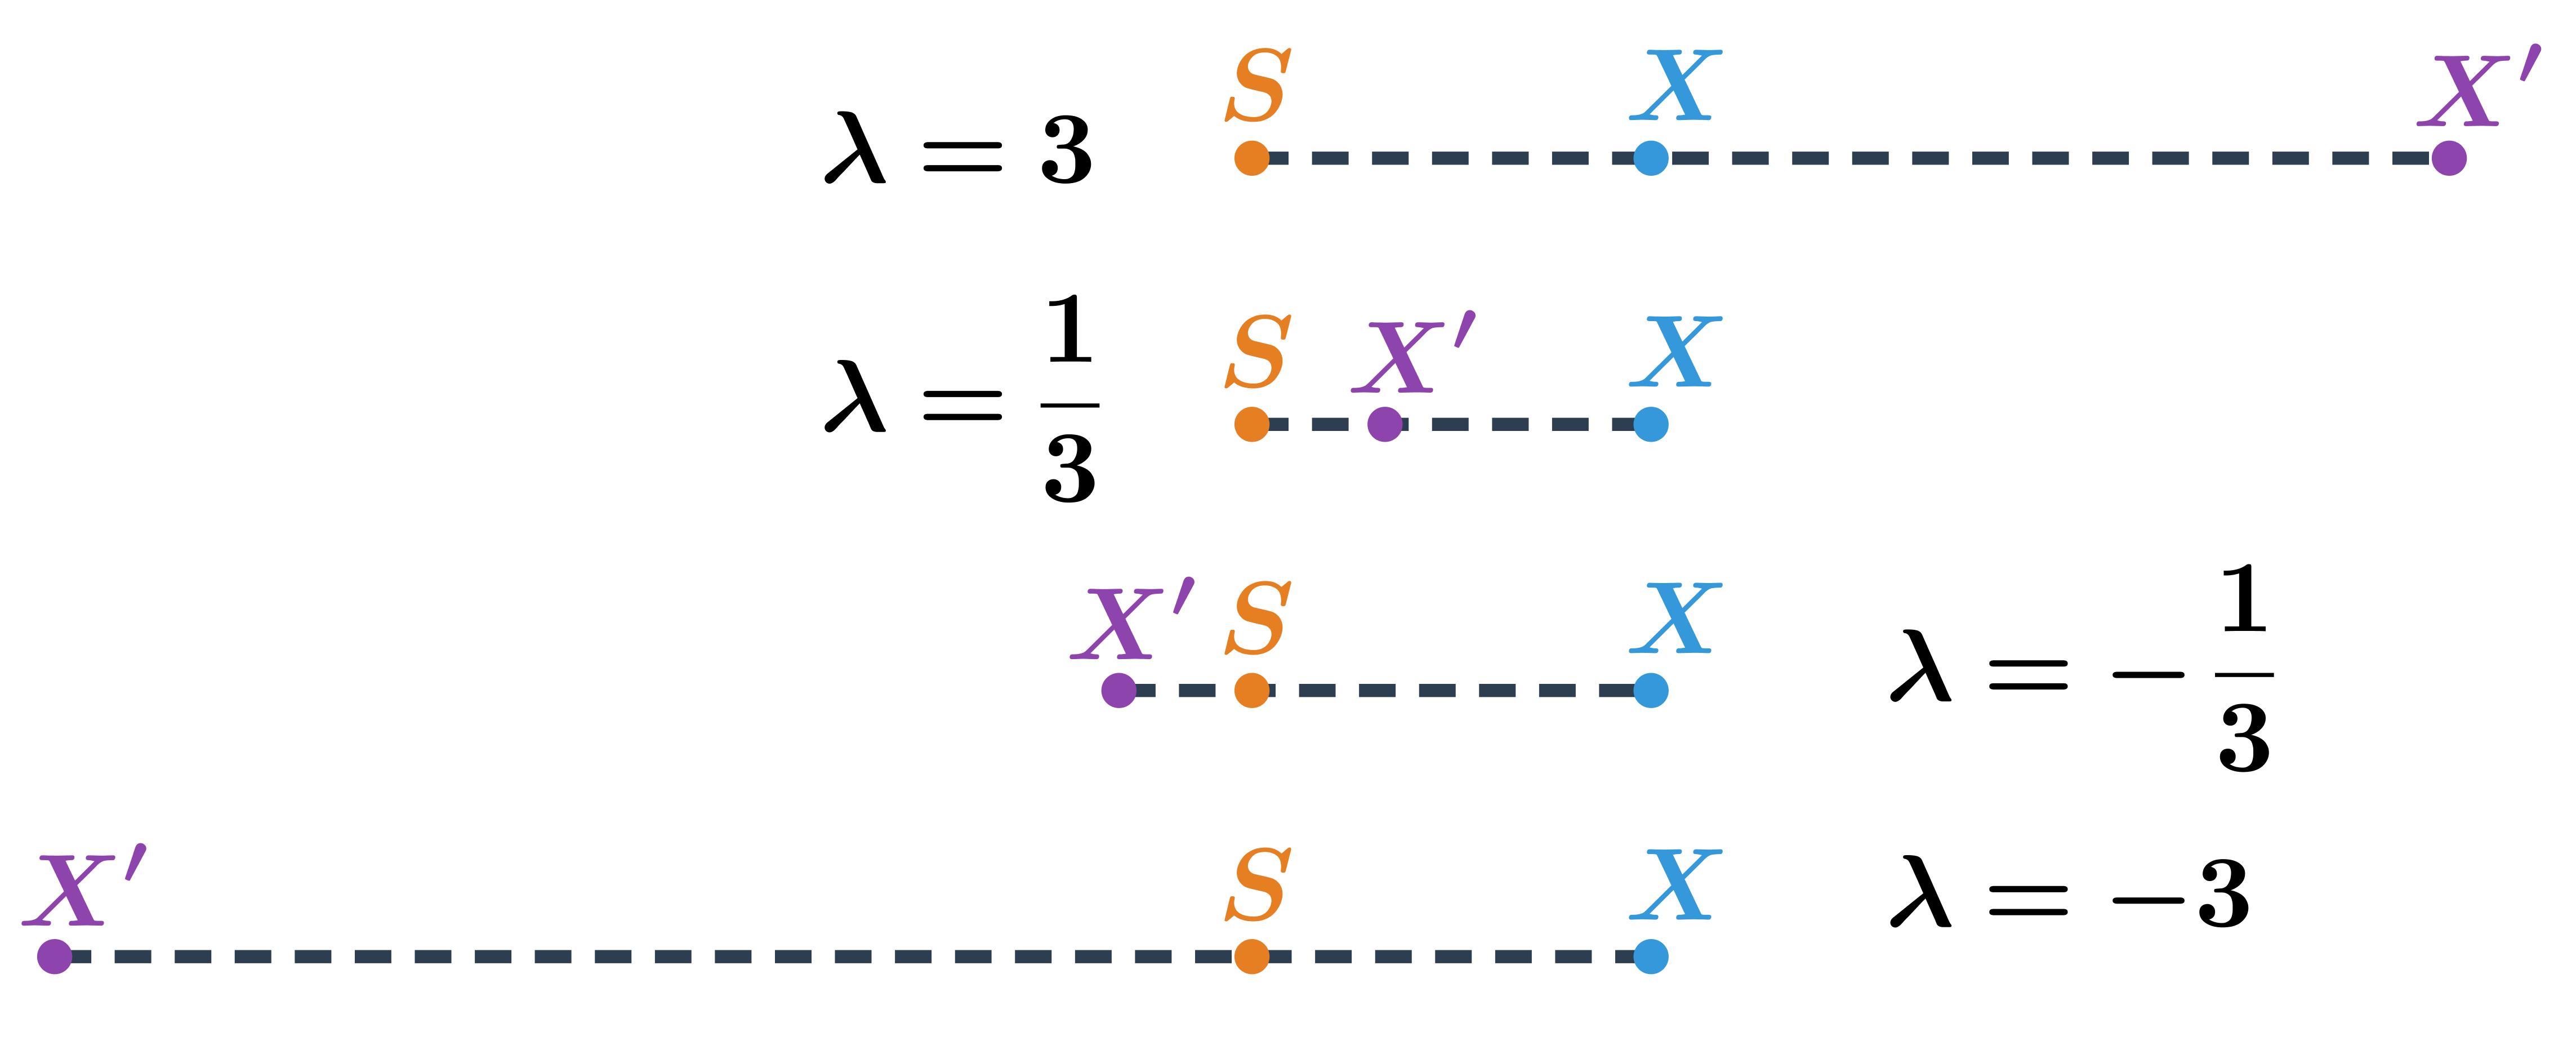
\includegraphics[width=0.5\linewidth]{stejnolehlost.png}
\end{center}
\end{reseni}

\begin{priklad}
Je dána kružnice $k$ a uvnitř ní bod $M$. Sestrojte všechny tětivy této kružnice
procházející bodem $M$, které jsou jím děleny v poměru $3:5.$
\end{priklad}

\begin{reseni}
Označme tětivu jako $XY$ ($X,Y$ jsou tedy na kružnici $k$). Pak $Y$ je obraz
bodu $X$ ve stejnolehlost se středem $M$ a koeficientem $-\frac{5}{3}$. Protože
body $X$ leží na kružnici $k,$ pak bod $Y$ leží na kružnici $k^\prime$ (tj. obraz
kružnice $k$ ve výše popsané stejnolehlosti). Proto je $Y$ průsečík $k\cap k^\prime$.
\end{reseni}

\begin{priklad}
Je dán konvexní úhel $\sphericalangle AVB$ a vnitřní bod $M$ tohoto úhlu. Sestrojte kružnici $k,M\in k,$
která se dotýká obou ramen úhlu.
\end{priklad}

\begin{reseni}
Sestrojíme si libovolnou kružnici $k^\prime$, která se dotýká ramen úhlu $AVB$ a pak
ji zobrazíme ve stejnolehlost se středem $V$ a koeficientem $\frac{|VM|}{|VM^\prime|},$
kde $M^\prime$ je průsečík úsečky $VM$ a kružnice $k^\prime$.
\end{reseni}

\begin{priklad}
Je dána přímka $p$, kružnice $k$, která nemá s přímkou $p$ společný bod a bod $A$, který
neleží ani na přímce $p$, ani ve vnitřní oblasti kružnice $k$. Sestrojte trojúhelník
$ABC$ s~úhlem $|\sphericalangle BAC|=60^\circ$ tak, aby $B\in p, C \in k, |AC|=2|AB|.$
\end{priklad}

\begin{reseni}
Bod $C$ je obraz bodu $B$ ve složeném zobrazení ze stejnolehlosti se středem v bodě
$A$ a koeficientem 2 a následném otočení o $60^\circ.$ \dots Proto je bod $C$ průsečík
kružnice $k$ a přímky $p^\prime$ získené výše popsaným zobrazením.
\end{reseni}

\section{Kartézský součin, binární relace, zobrazení}
\begin{definition}
  \textbf{Kartézským součinem množin} $A,B$ nazýváme množinu $A\times B$ všech uspořádaných dvojic $(a,b)$ takových, že $a\in A,b\in B$.
  \[
    A\times B=\left{ (a,b): a\in A,b\in B \right}
  \]
\end{definition}

\begin{pozn}
  Kartézský součin $A\times A$ nazveme \textbf{kartézským čtvercem} množiny $A$.
\end{pozn}

\begin{pozn}
  Kartézský graf je graf, kde prvky na ose $x$ (resp. $y$) jsou prvky z množiny $A$ (resp. $B$) a uspořádanou dvojici $(a,b)$ zaneseme jako příslušný bod se souřadnicemi $[a,b].$
\end{pozn}

\begin{definition}
  Nechť $A,B$ jsou dvě množiny. Pak každou podmnožinu $A\times B$ nazýváme \textbf{binární relací} mezi množinami $A,B$ (v tomto pořadí). Je-li speciálně $A=B$, pak hovoříme o \textbf{binární relaci v množině} $A$.
\end{definition}

\begin{definition}
  Relace na množině $A$ je
  \begin{enumerate}[$i.$]
    \item \textbf{reflexivní}, pokud $\forall a\in A: a\sim a$,
    \item \textbf{symetrická}, pokud $\forall a,b \in A: a\sim b \implies b\sim a,$
    \item \textbf{tranzitivní}, pokud $\forall a,b,c\in A: a\sim b \land b\sim c \implies a\sim c.$
  \end{enumerate}
\end{definition}

\begin{definition}
  Relaci na množině $A$, která je zároveň reflexivní, symetrická a tranzitivní nazveme \textbf{relací ekvivalence}.
\end{definition}

\begin{pozn}
  Každé relaci ekvivalence na množině $A$ přísluší \textbf{rozklad příslušný ekvivalenci} tak, že množinu $A$ rozdělíme na po dvou disjunktní podmnožiny, jejichž sjednocení dává množinu $A$ a navíc platí, že všechny prvky v jedné podmnožině jsou navzájem ekvivalentní a žádné dva prvky z jiných podmnožin ekvivalentní nejsou.
\end{pozn}

\begin{definition}
  Nechť $A,B$ jsou dvě množiny. \textbf{Zobrazením} $f$ \textbf{z množiny $A$ do množiny $B$} nazýváme relaci $f\subseteqA\times B,$ pro níž platí: $\forall x\in A: \exists \text{ max. 1 }y\in B: (x,y)\in f$. Prvek $x$ nazveme \textbf{vzorem} a $y$ \textbf{obrazem}.
\end{definition}

\begin{definition}
  Nechť $f\subseteq A\times B$ je zobrazení. \textbf{Definičním oborem} (resp. \textbf{oborem hodnot}) zobrazení $f$ nazveme množinu $D(f)\subseteq A$ (resp. $H(f)\subseteq B$) všech prvků $a\in A$ (resp. $b\in B$) tak, že k nim existuje právě jedno $b\in B$ (resp. alespoň jedno $a\in A$) tak, že $b=f(a)$ (resp. $a=f(b)$).
\end{definition}

\begin{definition}
  Pokud $D(f) = A$ (resp. $D(f)\ne A$), hovoříme o \textbf{zobrazení množiny} (resp. \textbf{zobrazení z množiny}) $A$. Pokud $H(f)=B$ (resp. $H(f)\ne B$), hovoříme o \textbf{zobrazení na množinu} (resp. \textbf{zobrazení do množiny}) $B$. 
  Zobrazení na nazýváme \textbf{surjekcí}. Je li $A=B$, hovoříme o \textbf{zobrazení v množině} $A$.
\end{definition}

\begin{definition}
  Nechť $f$ je zobrazení z $A$ do $B$. Zobrazení $f$ je \textbf{prosté}, jestliže ke každému $b\in B$ existuje nejvýše jedno $a \in A$ tak, že $b=f(a).$
\end{definition}

\begin{definition}
  Zobrazení množiny do množiny, které je prosté, nazýváme \textbf{injekce}. Zobrazení, které je současně surjekcí a injekcí, nazýváme \textbf{bijekce}.
\end{definition}

\begin{definition}
  Nechť $\alpha \subseteq A\times B$ je binární relace. \textbf{Inverzní relací} k relaci $\alpha$ nazveme relaci $\alpha^{-1} \subseteq B\times A$ takovou, že 
  \[
    \alpha^{-1}=\left{ (b,a)\in B\times ;  (a,b\in \alpha)\right}.
  \]
  Je-li $\alpha^{-1}$ zobrazení, nazveme relaci $\alhpa ^{-1}$ \textbf{inverzním zobrazením} k zobrazení $\alpha$.
\end{definition}

\begin{definition}
  Nechť $f:A\to B, g:B\to C$ jsou zobrazení. \textbf{Složeným zobrazením} ze zobrazení $f$ g $g$ nazveme relaci $h\subseteq A\times C$ takovou, že
  \[
    h=\left{ (a,c)\in A\times C;\exists b\in B: f(a)=b \land g(b)=c \right}.
  \]
  Značíme $c=g(f(a))$, $h=g\, \circ \, f $ (čteme \uv{$g$ po $f$}).
\end{definition}



\section{Funkce a jejich základní vlastnosti}
\begin{definition}
  \textbf{Funkcí} $f$ nazýváme každé zobrazení z $\mathbb R$ do $\mathbb R$.
\end{definition}

\begin{pozn}
  Obecněji by se funkce dala definovat také jako zobrazení z $\mathbb C$ do $\mathbb C$.
\end{pozn}

\begin{definition}
  Nechť $f\subseteq \mathbb R \times \mathbb R$ je funkce. Množinu
  \[
    D(f) = \left  \{ x \in \mathbb R:\exists ! y \in \mathbb R:y=f(x) \right \}
  \]
  nazveme \textbf{definičním oborem} funkce $f$. Množinu
  \[
    H(f) = \left  \{ y \in \mathbb R:\exists  x \in \mathbb R:y=f(x) \right \}
  \]
  nazveme \textbf{oborem hodnot} funkce $f$.
\end{definition}

\begin{priklad}
Určete definiční obor a obor hodnot funkce $y=x^2+x+1.$
\end{priklad}

\begin{reseni}
Definiční obor je $\mathbb R$, obor hodnot (množinu všech vyhovujících $a$)
získáme řešením rovnice $a=x^2+x+1.$
\end{reseni}

\begin{pozn}
  \textbf{Grafem funkce} rozumíme množinu všech bodů $[x,f(x)]$, kde $x\in D(f).$
\end{pozn}

\begin{priklad}
Nakreslete graf funkce $y=2-|x+1|.$
\end{priklad}

\begin{priklad}
Nakreslete graf funkce $y=-2x^2+x-1$.
\end{priklad}

\begin{reseni}
Doplněním na čtverec, odkud jsou posuny jasně patrné.
\end{reseni}

\begin{definition}
  Funkce $f$ se nazývá \textbf{lichá} (resp. \textbf{sudá}), jestliže platí
  \begin{enumerate}[$i.$]
    \item $\forall x \in D(f): -x \in D(f)$ a
  	\item $\forall x \in D(f): f(-x)=-f(x)$, resp. $f(-x)=f(x)$.
  \end{enumerate}
\end{definition}

\begin{pozn}
  Graf liché funkce je souměrný podle počátku, graf sudé funkce je souměrný podle souřadné osy $y$.
\end{pozn}

\begin{priklad}
Určete paritu funkce $y=x^2$.
\end{priklad}

\begin{reseni}
\begin{enumerate}[1.]
\item $D(f)=\mathbb R$ -- platí,
\item $f(-x)=(-x)^2=x^2=f(x)$ -- platí, tedy funkce je sudá.
\end{enumerate}
\end{reseni}

\begin{definition}
  Funkce $f$ se nazývá \textbf{prostá}, právě tehdy když
  \[
    \forall x_1,x_2\in D(f): x_1\ne x_2 \implies f(x_1)\ne f(x_2).
  \]
\end{definition}

\begin{definition}
  Nechť $f$ je funkce a $M$ alespoň dvouprvková množina z $D(f)$. Řekneme, že funkce $f$ je na množině $M$
  \begin{enumerate}[$i.$]
    \item \textbf{rostoucí} $\iff \forall x_1, x_2 \in M: x_1 < x_2 \implies f(x_1) < f(x_2),$
    \item \textbf{klesající} $\iff \forall x_1, x_2 \in M: x_1 < x_2 \implies f(x_1) > f(x_2),$
    \item \textbf{neklesající} $\iff \forall x_1, x_2 \in M: x_1 < x_2 \implies f(x_1) \leq f(x_2),$
    \item \textbf{nerostoucí} $\iff \forall x_1, x_2 \in M: x_1 < x_2 \implies f(x_1) \geq f(x_2).$
  \end{enumerate}
  Je-li $f$ neklesající nebo nerostoucí, je \textbf{monotónní}. Pokud je klesající nebo rostoucí, je \textbf{ryze monotónní}.
\end{definition}

\begin{priklad}
Určete monotónnost funkce $y=x^2$ na množině $\mathbb R_0^+.$
\end{priklad}
\begin{reseni}
Je-li $x_1,x_2 >0$, pak $x_1 < x_2 \implies x_1^2 < x_1x_2.$ Obdobně $x_1x_2<x_2^2$.
Celkem tedy $x_1^2<x_2^2 \implies f(x_1)<f(x_2),$ tedy $f$ je rostoucí v $\mathbb R_0^+.$
\end{reseni}

\begin{definition}
  Nechť $f$ je funkce, $M\subseteq D(f)$. Řekneme, že funkce $f$ je na množině $M$
  \begin{enumerate}[$i.$]
    \item \textbf{shora omezená} $\iff \exists k \in \mathbb R: \forall x \in M: f(x)\leq k,$
    \item \textbf{zdola omezená} $\iff \exists k \in \mathbb R: \forall x \in M: f(x)\geq k,$
    \item \textbf{omezená} $\iff $ je zdola i shora omezená.
  \end{enumerate}
\end{definition}

\begin{definition}
  Nechť $f$ je funkce, $M \subseteq D(f)$, v ní prvek $a \in M$.
  Řekneme, že funkce $f$ má v bodě $a$:
  \begin{enumerate}[$i.$]
    \item \textbf{ostré maximum} na množině $M$ právě tehdy, když $\forall x \in M\smallsetminus \left \{ a \right \}  : f(x) < f(a)$,
    \item \textbf{maximum} (neostré) na množině $M$ právě tehdy, když $\forall x \in M \smallsetminus \left \{ a \right \}: f(x) \leq f(a)$,
    \item \textbf{ostré minimum} na množině $M$ právě tehdy, když $\forall x \in M\smallsetminus \left \{ a \right \}: f(x) > f(a)$,
    \item \textbf{minimum} (neostré) na množině $M$ právě tehdy, když $\forall x \in M\smallsetminus \left \{ a \right \} : f(x) \geq f(a)$.
  \end{enumerate}
\end{definition}

\begin{definition}
  Nechť $f$ je funkce. Funkce $f$ se nazývá \textbf{periodická}, pokud $\exists p \in \mathbb R^{+}: \forall x \in D(f):$
  \begin{enumerate}
    \item $x \in D(f) \implies x \pm p \in D(f)$ a
    \item $f(x) = f(x \pm p)$.
  \end{enumerate}
  Číslo $p$ se nazývá \textbf{periodou} této funkce. Periodu $p_0$ nazveme \textbf{nejmenší periodou} funkce, pokud pro všechny ostatní periody $p$ platí $p > p_0$. V opačném případě se funkce nazývá \textbf{neperiodická}.
\end{definition}

\begin{definition}
  Nechť máme funkci $f: y = f(u)$ s definičním oborem $D(f)$ a funkci $g: u=g(x)$ s oborem hodnot $H(g)$. Jestliže je $H(g) \subseteq D(f)$, pak funkci $h: y = f(g(x))$ nazveme \textbf{složenou funkcí} (někdy píšeme též $h=f \circ g$).
\end{definition}

\begin{definition}
  \textbf{Dirichletova funkce} je definována následovně:
  $$\mathbf{D} (x) = \begin{cases}
1, & \text{ je-li } x \in \mathbb Q, \\
0 & \text{ jinak}.
  \end{cases}  $$
\end{definition}

\begin{definition}
  Funkce \textbf{signum} je definována následovně: $$\operatorname {sgn} x={\begin{cases}-1,& \textrm{je-li }x<0,\\0,&\textrm{je-li }x=0,\\1,&\textrm{je-li }x>0.\end{cases}}$$
\end{definition}

\begin{definition}
  Nechť $x \in \mathbb{R}$ je libovolné číslo. Pak existuje právě jedna dvojice $z \in \mathbb{Z}, a \in \left \langle 0;1 \right) \text{ tak, že } x = z + a$.
Číslo $z$ nazýváme \textbf{celou částí} čísla $x$ a zapisujeme $[x] = z$, někdy taky $\lfloor x \rfloor = z$.
\end{definition}

\begin{pozn}
    Pro definici limity a funkce spojité viz kapitolu \ref{limita},
    dále definici derivace def. \ref{derivace}, funkce konvexní a
    konkávní def. \ref{konvkonk} a konečně definici integrálu def. \ref{integral}.
\end{pozn}

\section{Polynomy, kořeny polynomů}
\begin{definition}
  \textbf{Polynomem} nazýváme každý výraz $P(x)$ tvaru
  \[
    P(x)=a_nx^n + a_{n-1}x^{n-1}+\dots + a_2x^2+a_1x+a_0,
  \]
  kde $a_i\in \mathbb R, i\in \{ 0,1,\dots , n \},n\in \mathbb N$. Čísla $a_i$ se nazývají \textbf{koeficienty polynomu}, sčítance $a_ix^i$ \textbf{členy polynomu}. Je-li $a_n\ne 0$, číslo $n$ se nazývá \textbf{stupeň polynomu} a označuje se $n= \text{st}(P(x))$. Je-li $a_i=0$ pro všechna $i \in \{ 0,1,\dots ,n\}$, pak klademe $\text{st}(P(x))=-\infty$ a $P(x)$ se nazývá \textbf{nulovým polynomem}. Označujeme jej $O(x).$ Je-li $a_n=1$, nazývá se $P(x)$ \textbf{normovaným polynomem}.
\end{definition}

\begin{veta}[O dělení polynomů se zbytkem]
  Nechť $A(x), B(x) \in \mathbb R[x],B(x) \ne O(x).$ Pak existuje právě jedna dvojice polynomů $Q(x),R(x)\in \mathbb R[x]$ tak, že
  \[
    A(x)=B(x)\cdot Q(x)+R(x),
  \]
  kde $R(x)=O(x)$ nebo $\text{st}(R(x))<\text{st}(B(x)).$
\end{veta}

\begin{definition}
  Nechť $A(x), B(x) \in \mathbb R[x]$. Řekneme, že polynom $B(x)$ \textbf{dělí} polynom $A(x)$ právě tehdy, když existuje takový polynom $C(x) \in \mathbb R[x]$ tak, že
  \[
    A(x) = B(x)\cdot C(x).
  \]
  Zapisujeme $B(x) \, | \, A(x).$
\end{definition}

\begin{definition}
  Nechť $P(x)\in \mathbb R[x], P(x)=a_nx^n+a_{n-1}x^{n-1}+\dots +a_1x+a_0.$ Nechť $c\in \mathbb R$ je libovolné číslo. \textbf{Hodnotou polynomu} $P(x)$ \textbf{v čísle} (v bodě) $c$ nazýváme reálné číslo $P(c)$
  \[
    P(c) = a_nc^n+a_{n-1}c^{n-1}+\dots+a_1c+a_0.
  \]
  Číslo $c\in \mathbb R$ nazveme \textbf{kořenem polynomu} $P(x) \iff P(c) = 0$.
\end{definition}


\begin{definition}
  Nechť $P(x) \in \mathbb R [x]$ a $c\in \mathbb R$ je jeho kořen. Lineární polynom $x-c$ nazveme \textbf{kořenovým činitelem}.
\end{definition}

\begin{definition}
  Nechť $P(x) \in \mathbb R [x], c \in \mathbb R$ je jeho kořen a $k \in \mathbb N$. Číslo $C \in \mathbb R$ nazýváme \textbf{$k$-násobným kořenem} polynomu $P(x)$ právě tehdy, když platí
  \[
    (x-c)^k \, | \, P(x) \land (x-c)^{k+1} \nmid  P(x).
  \]
\end{definition}

\begin{veta}[Vi\`{e}tovy vztahy]
  Nechť $P(x)=a_nx^n+a_{n-1}x^{n-1}+\dots + a_1x+a_0$ je polynom stupně $n$, který má v množině $\mathbb R$ právě $n$ kořenů $x_1,x_2\dots,x_n$ (každý počítáme tolikrát, jaká je jeho násobnost). Pak platí:
  \begin{align*}
    \sum_{i=1}^n x_i = & -\frac{a_{n-1}}{a_n} \\
    \sum_{i,j=1; i<j}^{n}x_ix_j= & \frac{a_{n-2}}{a_n} \\
    \vdots & \\
    \prod_{i=1}^nx_i=&(-1)^n\frac{a_0}{a_n}
  \end{align*}
\end{veta}

\begin{pozn}
  \textbf{Hornerovo schéma} je numerická metoda pro vyhodnocení funkční hodnoty polynomu $P(x) \in \mathbb R [x]$ v bodě $ x_0 \in \mathbb R$. Příklad:
  Vyhodnoťte $f_{1}(x)=2x^{3}-6x^{2}+2x-1$ v bodě $x=3$.
  Opakovaným vytknutím $x$, může být $f_{1}$ zapsáno jako $x(x(2x-6)+2)-1$. Pro větší přehlednost užijeme k zápisu průběhu výpočtu tzv. syntetický diagram.
  \begin{center}
    \begin{tabular}{ c|c c c c }
        $x_{0}$ & $x^{3}$ & $x^{2}$ & $x^{1}$ & $x^{0}$\\
        \hline
        $3$ & $2$ & $0$ & $2$ & $5$
    \end{tabular}
  \end{center}
  Do prvního místa opíšeme $a_n$. Čísla v řádku jsou součty koeficientu $a_k$ součinu hodnoty $x$, v níž polynom vyhodnocujeme (v tomto příkladě tedy $3$) s číslem v řádku o jeden sloupec vlevo (tedy pod $a_{k+1}$). Výsledek vyhodnocování je vpravo dole – v našem případě tedy $5$.

  Důsledkem věty o dělení polynomu polynomem je, že zbytek po vydělení f1 polynomem (x-3) je 5 a výsledkem tohoto dělení je polynom stupně 2 s koeficienty danými zbylými třemi čísly ve třetím řádku. Díky tomuto pozorování lze Hornerovo schéma použít i jako efektivní algoritmus k dělení polynomů.
\end{pozn}

\begin{veta}
    Nechť je dána algebraická rovnice
    \begin{equation}\label{alg_rce}
        a_nx^n + a_{n-1}x^{n-1}+\dots + a_1x+a_0=0,
    \end{equation}
    $a_n \ne 0$ s celočíselnými koeficienty. Nechť $\frac{r}{s}, r\in \mathbb Z, s \in \mathbb N, D(r,s)=1$ je kořenem této rovnice.
    Pak platí: $r \, | \, a_0 \land s \, |\, a_n.$
\end{veta}

\begin{veta}\label{odecitanivpolynomu}
    Nechť $\frac{r}{s}$ je racionální kořen algebraické rovncie \ref{alg_rce} s celočíselnými koeficienty.
    Nechť $m$ je pevné celé číslo. Pak platí:
    $$(r-ms) \, |\, a(m),$$
    kde $a(m)$ je hodnota polynomu $a(x)$ pro $x=m.$ Dále $r \, | \, a_0$ a $s\, |\, a(-1).$
\end{veta}

\begin{comment}
\begin{veta}[Hledání racionálních kořenů polynomu s racionálními koeficienty]
  Mějme polynom $P(x) \in \mathbb Q [x]$. Potom najdeme jeho kořeny $\frac{r}{s} \in \mathbb Q$ takto:
  \begin{enumerate}[1.]
    \item Nalezneme všechny celočíselné dělitele $r$ absolutního členu polynomu $a_0$.
    \item Nalezneme všechny přirozené dělitele $s$ vedoucího členu $a_n$.
    \item Utvoříme všechny zlomky tvaru $\frac{r}{s}, (r,s) = 1$.
    \item Hornerovým schématem určíme $P(1)$, případně $P(-1)$ ($1$ a $-1$ také mohou být kořeny).
    \item Vyškrtáme ty zlomky $\frac{r}{s}$, které nesplňují podmínky $(r-s) \mid P(1) \land (r+s) \mid P(-1)$.
    \item U ostatních zlomků vyzkoušíme Hornerovým schématem, zda jsou kořeny daného polynomu.
  \end{enumerate}
\end{veta}
\end{comment}

\begin{priklad}
Najděte racionální kořeny polynomu $P(x)=\frac{3}{5}x^4+x^3+\frac{1}{5}x^2+x-\frac{2}{5}.$
\end{priklad}

\begin{reseni}
Vynásobme polynom 5, abychom měli všechny koeficienty celé.
$$P(x) = 3x^4+5x^3+x^2+5x-2.$$
Pak $r \, | \, a_0 \implies r\, | \, -2 \implies r \in \left \{ \pm 2, \pm 1 \right \} $
a $s \, | \, a_n\implies s \, | \, 3 \implies s \in \left \{ 1, 3 \right \} $.
Sestavíme všechny možnosti a vyzkoušíme. S výhodou taky můžeme využít věty
\ref{odecitanivpolynomu}.
\end{reseni}


\begin{veta}[Rozklad polynomu v reálném a komplexním oboru]
  Nechť $P(x) \in \mathbb R [x]$,
  $$P(x) = a_n x^n + a_{n-1} x^{n-1} + \dots + a_1 x + a_0,$$
  kde $\textrm{st}(P(x)) \geq 1$. Pak $P(x)$ lze v $\mathbb R$ vyjádřit jako součin polynomů 1. a 2. stupně a koeficientu $a_n$ následovně:
  \begin{align*}
    P(x) & = a_n(x-c_1)^{k_1}(x-c_2)^{k_2} \dots (x-c_k)^{k_k}\\
    & \cdot (x^2+p_1 x + q_1)^{r_1}(x^2+p_2 x + q_2)^{r_2} \dots (x^2+p_r x + q_r)^{r_r},
  \end{align*}


  kde $c_1,c_2, \dots, c_k$ jsou všechny jeho reálné různé kořeny s násobnostmi $l_1, k_2, \dots, k_k \in \mathbb N$;
  $p_1, p_2, \dots, p_r$ a $q_1, q_2, \dots, q_r$ jsou reálná čísla, $r_1, r_2, \dots, r_n \in \mathbb N$.
  Polynomy
  $$(x^2+p_1 x + q_1)^{r_1}(x^2+p_2 x + q_2)^{r_2} \dots (x^2+p_r x + q_r)^{r_r}$$
  jsou kvadratické polynomy se záporným diskriminantem. Uvedený rozklad je až na pořadí činitelů
  jednoznačný a platí
  $$\textrm{st}(P(x)) = k_1 + k_2 + \dots + k_k + 2(r_1 + r_2 + \dots + r_r).$$

  Jestliže $a_1 \pm ib_1, a_2 \pm ib_2, \dots, a_s \pm ib_s$ jsou všechny navzájem různé
  dvojice komplexně sdružených kořenů s násobností $r_1, r_2, \dots, r_s$, $P(x)$ můžeme v $\mathbb C$ psát ve tvaru:
  \begin{align*}
    P(x) & = a_n(x-c_1)^{k_1}(x-c_2)^{k_2} \dots (x-c_k)^{k_k}\\
    & \cdot  \left [(x-a_1)^2+b_1^2\right ]^{r_1}\left [(x-a_2)^2+b_2^2\right]^{r_2} \dots \left [(x-a_s)^2+b_s^2\right ]^{r_s}
  \end{align*}
\end{veta}

\begin{priklad}
    Určete, pro která $x \in \mathbb R$ platí:
    $$P(x)=(x-1)^2(x+5)^3x^4(x^2-5x+6)(x^2+1)(x-5)^5 \geq 0.$$
\end{priklad}

\begin{reseni}
Rozložíme v reálném oboru. Členy se záporným diskriminantem nemají reálný kořen,
neuvažujeme je tedy. V sudých mocninách se nemění znaménko.
\end{reseni}

\begin{definition}
  Nechť $A(x), B(x) \in \mathbb R [x]$. Polynom $C(x) \in \mathbb R [x]$ se nazývá \textbf{společný dělitel polynomů} $A(x), B(x)$
  právě tehdy, když platí: $C(x) \mid A(x) \land C(x) \mid B(x)$.
  Polynom $D(x) \in \mathbb R [x]$ se nazývá \textbf{největší společný dělitel polynomů} $A(x), B(x)$, který označujeme $D(A(x), B(x))$ nebo $(A(x), B(x))$, právě tehdy, když platí:
  \begin{enumerate}[i.]
    \item $D(x) \mid A(x) \land D(x) \mid B(x)$ a
    \item $\forall C(x) \in \mathbb R [x]: C(x) \mid A(x) \land C(x) \mid B(x) \implies C(x) \mid D(x).$
  \end{enumerate}
\end{definition}

\begin{pozn}
  Největší společný dělitel hledáme \textbf{Euklidovým algoritmem}: Nechť $A(x), B(x) \in \mathbb R [x]$.
  \begin{enumerate}[a.]
    \item $A(x) = O(x) \implies D(A(x), B(x)) = B(x)$
    \item $\text{st}(A(x)) \geq \text{st}(B(x)) \geq 0$
  \end{enumerate}
  Proveďme následující posloupnost dělení se zbytkem. Toto dělení ukončíme, až bude zbytek nulový polynom.
  Vzhledem k nerovnosti na pravé straně tento nulový zbytek existuje.

  \begin{minipage}{0.6\textwidth}
  \begin{align*}
    A(x) & = B(x) \cdot Q_1(x) + R_1(x),  \\
    B(x) & = R_1(x) \cdot Q_2(x) + R_2(x),  \\
    R_1(x) & = R_2(x) \cdot Q_3(x) + R_3(x), \\
    \dots & = \dots \\
    R_{n-2}(x) & = R_{n-1}(x) \cdot Q_n(x) + R_n(x),  \\
    R_{n-1}(x) & = R_{n}(x) \cdot Q_{n+1}(x),
  \end{align*}
  \end{minipage}
  \hfill
  \begin{minipage}{0.38\textwidth}
  \begin{align*}
   \text{st}(R_1(x)) & < \text{st}(B(x)) \\
   \text{st}(R_2(x)) & < \text{st}(R_1(x)) \\
 \text{st}(R_3(x)) & < \text{st}(R_2(x)) \\
    \dots & < \dots \\
 \text{st}(R_n(x)) & < \text{st}(R_{n-1}(x)) \\
   R_{n}(x) & < O(x).
  \end{align*}
  \end{minipage}

  Potom $(A(x), B(x)) = R_n(x)$, či libovolný násobek $R_n(x)$. \textbf{Normovaný největší společný dělitel polynomů}
  ale existuje právě jeden, ten se označuje $(A(x), B(x))$.
\end{pozn}

\begin{priklad}
    Určete největšího společného dělitele polynomů
    \begin{equation*}
        x^3+8x^2+17x+10,\\
        x^3+5x^2+2x+10.
    \end{equation*}
\end{priklad}

\begin{reseni}
Euklidovým algoritmem. Dělíme tak dlouho, dokud nevyjde nulový zbytek.
Mezi jednotlivými děleními můžeme polynomy vynásobit libovolnou konstantou (protože
to nezmění kořeny polynomu).
\end{reseni}

\begin{definition}
  Nechť polynomy $A(x), B(x)$. Pokud $(A(x), B(x)) = 1$, řekneme, že polynomy $A(x), B(x)$ jsou \textbf{nesoudělné}. V opačném případě jsou \textbf{soudělné}.
\end{definition}

\begin{definition}
    Nechť $P(x) \in \mathbb R[x], P(x)=a_nx^n+a_{n-1}x^{n-1}+\dots+a_1x+a_0.$ \textbf{Derivací polynomu} $P(x)$ rozumíme polynom $P^\prime(x)$ definovaný takto:
    $$
        P^\prime(x)=\begin{cases}
        0, &\text{ je-li st} (P(x)) \leq 0,\\
        a_n n x^{n-1} + a_{n-1}(n-1)x^{n-2} + \dots + a_1, & \text{ je-li st} (P(x)) \geq 1.
        \end{cases}
    $$
\end{definition}


\begin{veta}
    Nechť $P(x) \in R[x], c \in \mathbb R$ je jeho $k$-násobný kořen, $k\in \mathbb N.$ Pak platí: $c$ je
    $k$-násobný kořen $P(x) \iff P(c)=P^\prime(c)=P^{\prime \prime}(c)=\dots= P^{k-1}(c)=0 \land P^{k}(c)\ne 0$.
\end{veta}


\begin{priklad}
Je dán polynom $x^3+3x-2$, který má dvojnásobný kořen.
Určete všechny jeho kořeny.
\end{priklad}

\begin{reseni}
Určíme první derivaci. Dvojnásobný kořen je kořenem první derivace, ale ne naopak.
Vyzkoušíme tedy v Hornerovém schématu.
\end{reseni}

\section{Polynomická funkce}

\begin{definition}\,
\begin{enumerate}[$i.$]
  \item Nechť $b \in \mathbb R$. Funkci $f:y = b$ nazveme \textbf{konstantní funkcí}.
  \item Nechť $a, b \in \mathbb R, a \neq 0$. Funkci $f:y= ax + b$ nazveme \textbf{lineární funkcí}.
\end{enumerate}
\end{definition}

\begin{pozn}\,
  \begin{itemize}
    \item Definičním oborem konstantní i lineární funkce je $\mathbb R$. \\
          Oborem hodnot konstantní funkce je ${b}$.\\
          Oborem hodnot lineární funkce je $\mathbb R$.
    \item Grafem konstantní funkce je přímka rovnoběžná s osou $x$. \\
          Grafem lineární funkce je přímka, která není rovnoběžná s osou $x$ ani s osou $y$.
  \end{itemize}
\end{pozn}

\begin{veta}
  Nechť $f: y = ax + b, a \neq 0$ je lineární funkce. Pak platí:
  \begin{enumerate}[$i.$]
    \item $b=0 \implies f$ je lichá,\\
          $b \neq 0 \implies f$ není ani sudá, ani lichá;
    \item $a > 0 \implies f$ je rostoucí,\\
          $a < 0 \implies f$ je klesající;
    \item $f$ není ani shora, ani zdola omezená;
    \item $f$ nemá extrémy;
    \item $f$ není periodická.
  \end{enumerate}
\end{veta}

\begin{proof}\,
  \begin{enumerate}[$i.$]
    \item $b=0 \implies f:y= ax = f(x) \land -ax = -f(x) \implies f$ je lichá\\
          $b\neq 0 \implies f:y = ax + b = f(x) = -ax + b \implies f$ není sudá ani lichá
    \item $a>0 \implies x_1 < x_2 \implies ax_1 < ax_2 \implies ax_1 + b < ax_2 + b \implies f$ je rostoucí\\
          $a<0 \implies x_1 < x_2 \implies ax_1 > ax_2 \implies ax_1 + b > ax_2 + b \implies f$ je klesající
    \item Obor hodnot je $\mathbb R \implies f$ není omezená.
    \item Plyne z grafu.
    \item Plyne z grafu nebo z toho, že $f$ je ryze monotónní. \qedhere
  \end{enumerate}
\end{proof}

\begin{definition}
  Nechť $a,b,c \in \mathbb R, a \neq 0$. Pak funkci $f:y = ax^2 + bx+ c$ nazýváme \textbf{kvadratickou funkcí}.
\end{definition}

\begin{pozn}\,
  \begin{itemize}
    \item Definičním oborem kvadratické funkce je $\mathbb R$.
    \item Grafem kvadratické funkce je parabola.
  \end{itemize}
\end{pozn}

\begin{veta}
  Nechť $f:y = ax^2, a \neq 0$ je kvadratická funkce. Pak platí:
  \begin{center}
    \begin{tabularx}{\textwidth}{ l | l  l }
        \, & $a>0$ & $a<0$ \\
        \hline
        obor hodnot & $H(f) = \mathbb R^{+}_0$ & $H(f) = \mathbb R^{-}_0$ \\
        parita & sudá & sudá \\
        monotónnost & $x \in (-\infty, 0\rangle$ -- klesající & $x \in (-\infty, 0\rangle$ -- rostoucí \\
        \, & $x \in \langle 0, \infty)$ -- rostoucí & $x \in \langle 0, \infty)$ -- klesající \\
        omezenost & zdola omezená & zdola neomezená \\
        \, & shora neomezená & shora omezená \\
        extrémy &  ostré minimum v bodě $x_0=0$ & ostré maximum v bodě $x_0=0$ \\
        periodicita & neperiodická & neperiodická
    \end{tabularx}
  \end{center}
\end{veta}

\begin{proof}
    Dokážeme jen paritu a monotonii. Ostatní plyne z grafu.
    \begin{enumerate}
        \item[$i.$] parita: $D(f) = \mathbb R$ -- platí, $f(-x)=a(-x)^2=ax^2=f(x) \implies f$ je sudá
        \item[$ii.$] monotonie: \begin{itemize}
        \item $a>0 \land x\in \left (-\infty,0\right >$: \\
        Je-li $x_1<x_2$, pak $ax_1^2 > ax_2^2 \iff ax_1 <ax_2 \iff ax_1^2>ax_1x_2 \land ax_1x_2 > ax_2^2 \implies$ platí.
            \item $a>0 \land x\in \left <0,\infty\right )$: \\
            Je-li $x_1<x_2$, pak $ax_1^2 > ax_2^2 \iff ax_1 <ax_2 \iff ax_1^2>ax_1x_2 \land ax_1x_2 > ax_2^2 \implies$ platí.\qedhere
        \end{itemize}
    \end{enumerate}
\end{proof}

\begin{veta}
  Nechť $f:y = ax^2+bx+c, a \neq 0$ je kvadratická funkce. Pak platí:
  \begin{center}
    \begin{tabularx}{\textwidth}{ l | l  l }
        \, & $a>0$ & $a<0$ \\
        \hline
        obor hodnot & $H(f) = \left <c-\frac{b^2}{4a}, \infty \right)$ & $H(f) = \left (-\infty, c-\frac{b^2}{4a}\right >$ \\
        parita & obecně není ani sudá, ani lichá & \, \\
        monotónnost & $x \in \left (-\infty, -\frac{b}{2a} \right >$ -- klesající & $x \in \left (-\infty, -\frac{b}{2a} \right >$ -- rostoucí \\
        \, & $x \in \left < -\frac{b}{2a}, \infty \right )$ -- rostoucí & $x \in \left < -\frac{b}{2a}, \infty \right )$ -- klesající \\
        omezenost & zdola omezená & zdola neomezená \\
        \, & shora neomezená & shora omezená \\
        extrémy &  ostré minimum v bodě $x_0=-\frac{b}{2a}$ & ostré maximum v bodě $x_0=-\frac{b}{2a}$ \\
        periodicita & neperiodická & neperiodická
    \end{tabularx}
  \end{center}
\end{veta}

\begin{definition}
    Nechť $P(x)\in \mathbb R[x]$ je polynom. Pak funkci $f:y=P(x)$ nazveme \textbf{polynomickou funkcí}.
\end{definition}

\begin{pozn}\,
    \begin{enumerate}[$i.$]
        \item Definičním oborem polynomické funkce je $\mathbb R.$
        \item Jestliže je stupeň polynomu lichý, pak je obor hodnot $\mathbb R.$ Jestliže je sudý a $a_n > 0,$ je obor hodnot interval $\left <c,\infty \right )$,
        v opačném případě je to interval $\left (-\infty, c\right >$, kde $c \in \mathbb R$.
    \end{enumerate}
\end{pozn}

\begin{definition}
    Nechť $y=f(x)$ je polynomická funkce. Pak $c\in \mathbb R$ nazveme \textbf{nulovým bodem} polynomické funkce $f$ právě tehdy, když $f(c)=0.$
\end{definition}

\begin{pozn}
    Nulovým bodem polynomické funkce rozumíme kořen polynomu.
\end{pozn}

\section{Racionální lomená funkce}
\begin{definition}
    Nechť $k \in \mathbb R, k \ne 0.$ Pak funkcí $y=\frac{k}{x}$
    nazýváme \textbf{nepřímou úměrností} s~koeficientem $k$.
\end{definition}

\begin{definition}
    Nechť $a,b,c,d \in \mathbb R, c \ne 0, ad-bc \ne 0.$ Pak funkci
    $f:y=\frac{ax+b}{cx+d}$ nazýváme \textbf{lineární lomenou
    funkcí}.
\end{definition}

\begin{priklad}
Nakreslete graf funkce $f: y=\frac{2x+3}{x+1}.$
\end{priklad}

\begin{reseni}
Vydělením získáme přehled o posunech počátku.
\end{reseni}

\begin{pozn}
    \begin{itemize}
        \item $D(f)=\mathbb R - \left \{ -\frac{d}{c} \right \}$
       	\item $H(f)=\mathbb R - \left \{ \frac{a}{c} \right \}$
       	\item Grafem je rovnoosá hyperbola s asymptotami
        $x=-\frac{d}{c}, y=\frac{a}{c}.$
    \end{itemize}
\end{pozn}

\begin{veta}
    Lineární lomená funkce:
    \begin{enumerate}[$i.$]
        \item není ani sudá, ani lichá;
       	\item $bc-ad > 0 \implies$ klesající v
        $\left ( -\infty, -\frac{d}{c} \right ),
        \left ( -\frac{d}{c}, \infty \right ) $ \\
        $bc-ad < 0 \implies$ rostoucí v
        $\left ( -\infty, -\frac{d}{c} \right ),
        \left ( -\frac{d}{c}, \infty \right ) $;
       	\item není omezená ani shora, ani zdola;
       	\item nemá extrémy;
       	\item není periodická;
       	\item je prostá.
    \end{enumerate}
\end{veta}

\begin{definition}
    Nechť $P(x), Q(x) \mathbb R[x]$ jsou polynomy, $Q(x) \ne O(x).$
    Pak funkci $F:y=\frac{P(x)}{Q(x)}$ nazýváme \textbf{racionální
    lomenou funkcí}.
\end{definition}

\begin{definition}
    Racionální lomená funkce $f: y=\frac{P(x)}{Q(x)}, Q(x) \ne O(x)$
    se nazývá
    \begin{enumerate}[$i.$]
        \item \textbf{ryze lomená} racionální funkce
        $\iff \text{st}\left (P(x) \right ) <
        \text{st}\left (Q(x) \right )$;
       	\item \textbf{neryze lomená} racionální funkce
        $\iff \text{st}\left (P(x) \right ) \geq
        \text{st}\left (Q(x) \right )$.
    \end{enumerate}
\end{definition}


-- insert řešení rovnic a nerovnic v podílovém tvaru, nevim moc co to má být lol---

\begin{veta}[Rozklad na parciální zlomky]
    Nechť $f: y=\frac{P(x)}{Q(x)}, Q(x) \ne O(x)$ je ryze lomená
    racionální funkce, kde polynomy $P(x)$ a $Q(x)$ nemají společné
    kořeny. Nechť
    \begin{align*}
        Q(x) = & \, a_n(x-c_1)^{k_1}(x-c_2)^{k_2} \dots
        (x-c_l)^{k_l} \\
        \cdot & \, (x^2+p_1x + q_1)^{k_1}(x^2+p_2x+q_2)
        ^{k_2} \dots (x^2+p_sx+q_s)^{rs}
    \end{align*}
    je rozklad polynomu $Q(x)$ v reálném oboru. Pak existují čísla
    \begin{center}
        \begin{tabular}{l l l l}
            $C_{11}$, & $C_{12}$, & $\dots$, & $C_{1k_1}$, \\
            $C_{21}$, & $C_{22}$, & $\dots$, & $C_{2k_2}$, \\
            \,        & \,        & $\dots$  & \,          \\
            $C_{l1}$, & $C_{l2}$, & $\dots$, & $C_{lk_l}$; \\
            $P_{11}$, & $P_{12}$, & $\dots$, & $P_{1r_1}$, \\
            $P_{21}$, & $P_{22}$, & $\dots$, & $P_{2r_2}$, \\
            \,        & \,        & $\dots$  & \,          \\
            $P_{s1}$, & $P_{s2}$, & $\dots$, & $P_{sr_s}$; \\
            $Q_{11}$, & $Q_{12}$, & $\dots$, & $Q_{1r_1}$, \\
            $Q_{21}$, & $Q_{22}$, & $\dots$, & $Q_{2r_2}$, \\
            \,        & \,        & $\dots$  & \,          \\
            $Q_{s1}$, & $Q_{s2}$, & $\dots$, & $Q_{sr_s}$
        \end{tabular}
    \end{center}
    tak, že $\forall x \in \mathbb R$ platí
    \begin{align*}
        y = & \left [
              \frac{C_{11}}{x-c_1} + \frac{C_{12}}{(x-c_1)^2} +
              \dots + \frac{C_{1k_1}}{(x-c_1)^{k_1}} \right . \\
          & + \frac{C_{21}}{x-c_2} + \frac{C_{22}}{(x-c_2)^2} +
              \dots + \frac{C_{2k_2}}{(x-c_1)^{k_2}} \\
          & + \dots \\
          & + \frac{C_{l1}}{x-c_l} + \frac{C_{l2}}{(x-c_l)^2} +
              \dots + \frac{C_{lk_l}}{(x-c_l)^{k_l}} \\
          & + \frac{P_{11}x + Q_{11}}{x^2 + p_1x + q_1}
              + \frac{P_{12}x + Q_{12}}{(x^2 + p_1x + q_1)^2} + \dots
              + \frac{P_{1r_1}x + Q_{1r_1}}{(x^2 + p_1x + q_1)^{r_1}} \\
          & + \frac{P_{21}x + Q_{21}}{x^2 + p_2x + q_2}
              + \frac{P_{22}x + Q_{22}}{(x^2 + p_2x + q_2)^2} + \dots
              + \frac{P_{2r_2}x + Q_{2r_2}}{(x^2 + p_2x + q_2)^{r_2}} \\
          & + \dots \\
          & + \left . \frac{P_{s1}x + Q_{s1}}{x^2 + p_sx + q_s}
              + \frac{P_{s2}x + Q_{s2}}{(x^2 + p_sx + q_s)^2} + \dots
              + \frac{P_{sr_s}x + Q_{sr_s}}{(x^2 + p_sx + q_s)^{r_s}} \right ]
              \cdot \frac{1}{a_n}
    \end{align*}
\end{veta}

\begin{priklad}
Rozložte na parciální zlomky: $y=\frac{x-4}{x^2-5x+6}.$
\end{priklad}

\begin{reseni}
Platí
$$\frac{x-4}{x^-5x+6}=\frac{A}{x-2}+\frac{B}{x-3}.$$
Metodou porovnání koeficientů tedy řešíme rovnici $x-4=A(x-3)+B(x-2)$.
\end{reseni}

--- insert aplikace diferenciálního a integrálního počtu ---

\section{Mocniny, mocninná funkce}
\begin{minipage}{0.64\textwidth}
\begin{definition}
    Nechť $n\in \mathbb N.$ Pak funkci $f: y=x^n$ nazýváme \textbf{mocninnou funkcí}
    s~přirozeným exponentem.
\end{definition}

\begin{definition}
    Nechť $n\in \mathbb N.$ Pak funkci $f: y=x^{-n}=\frac{1}{x^n}$ nazýváme
    \textbf{mocninnou funkcí} s~celým záporným exponentem.
\end{definition}

\begin{definition}
    Nechť $\frac{p}{q}\in \mathbb Q, x \in \mathbb R^+.$ Pak funkci $f: y=
    x^{\frac{p}{q}}=\sqrt[q]{x^p}$ nazýváme \textbf{mocninnou funkcí}
    s racionálním exponentem.
\end{definition}
\end{minipage}
\hfill
\begin{minipage}{0.34\textwidth}
\vspace{-1em}\noindent\hfill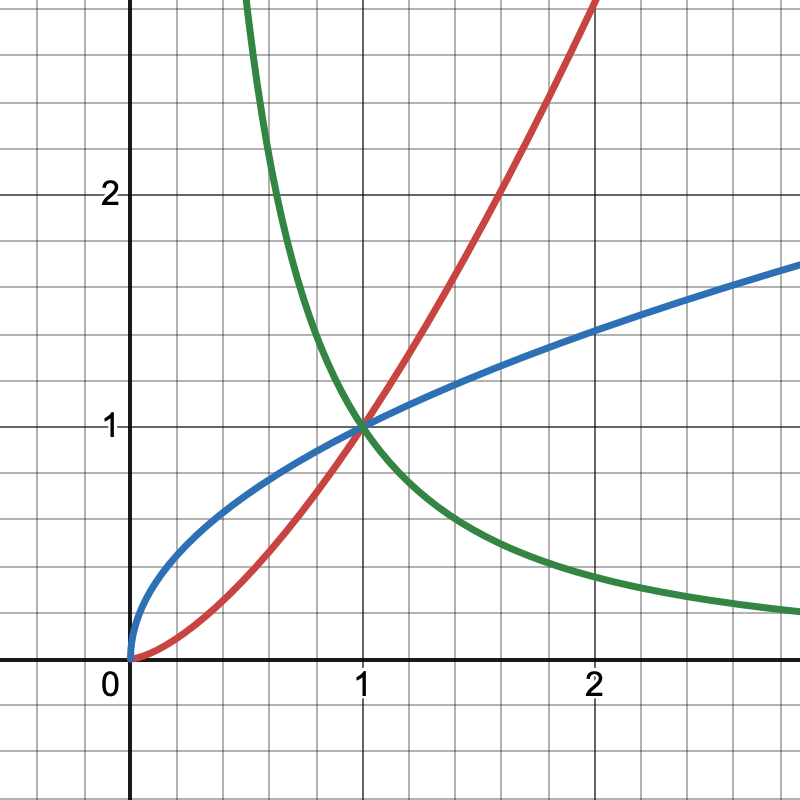
\includegraphics[width=0.95\linewidth]{mocninne_fce.png}
\end{minipage}

\begin{pozn}
    V grafu je červená funkce $y=x^\frac{2}{3}$, modrá funkce $y=x^\frac{1}{2}$ a
    zelená funkce $y=x^{-\frac{3}{2}}$.
\end{pozn}


\begin{veta}[Pravidla pro počítání s mocninami]
    $\forall a \in \mathbb R, m,n \in \mathbb N:$
    \begin{enumerate}[$i.$]
        \item $a^m\cdot a^n=a^{m+n};$
       	\item $(ab)^n = a^n\cdot b^n;$
       	\item $a^m : a^n = a^{m-n}, a \ne 0;$
       	\item $(a : b)^n = a^n : b^n, b \ne 0;$
       	\item $\left ( a^m \right )^n = a^{mn}.$
    \end{enumerate}
\end{veta}

\begin{proof}
    Zřejmé.
\end{proof}

\begin{veta}
  Vlastnosti mocninných funkcí $y= x^n$, kde $n$ je přirozené číslo:
  \begin{enumerate}[1.]
    \item Pokud $n$ je liché.
    \begin{enumerate}[$i.$]
      \item $D(f)= \mathbb R$, $H(f)= \mathbb R$.
      \item Je lichá.
      \item Není omezená shora ani zdola.
      \item Je rostoucí v celém svém definičním oboru.
      \item Nemá maximum, ani minimum.
    \end{enumerate}
    \item Pokud $n$ je sudé.
    \begin{enumerate}[$i.$]
      \item $D(f)= \mathbb R$, $H(f)= \langle 0,+\infty )$.
      \item Je sudá.
      \item Není omezená shora, je zdola omezená.
      \item Je rostoucí v intervalu $\langle 0,+\infty )$, je klesající v intervalu $( -\infty,0 \rangle $.
      \item Nemá maximum, má minimum v bodě $0$.
    \end{enumerate}
  \end{enumerate}
\end{veta}

\begin{veta}
  Vlastnosti mocninných funkcí $y= x^{-n}$, kde $n$ je přirozené číslo:
  \begin{enumerate}[1.]
    \item Pokud $n$ je liché.
    \begin{enumerate}[$i.$]
      \item $D(f)= \mathbb R - {0}$, $H(f)= \mathbb R - {0}$.
      \item Je lichá.
      \item Není omezená shora ani zdola.
      \item Je klesající v $( -\infty,0)$ a v $( 0,+\infty )$.
      \item Nemá maximum, ani minimum.
    \end{enumerate}
    \item Pokud $n$ je sudé.
    \begin{enumerate}[$i.$]
      \item $D(f)= \mathbb R - {0}$, $\mathbb H(f)= ( 0,+\infty )$.
      \item Je sudá.
      \item Není omezená shora, je zdola omezená.
      \item Je rostoucí v intervalu $( -\infty,0 ) $, je klesající v intervalu $( 0,+\infty )$.
      \item Nemá maximum ani minimum.
    \end{enumerate}
  \end{enumerate}
\end{veta}

\begin{definition}
    Nechť $n\in \mathbb N, n\geq 2, x \geq 0.$ Pak inverzní funkci k funkci
    $f:y=x^n$ nazýváme \textbf{$n$-tou odmocninou} a značíme $f^{-1}: y=\sqrt[n]{x}.$
\end{definition}

\begin{veta}[Pravidla pro počítání s odmocninami]
    $\forall a,b \in \mathbb R, a,b \geq 0, m,n \in \mathbb N:$
    \begin{enumerate}[$i.$]
        \item $\sqrt[m]{a}\cdot \sqrt[m]{b}=\sqrt[m]{ab};$
       	\item $\sqrt[m]{\sqrt[n]{a} } = \sqrt[mn]{a};$
       	\item $\sqrt[m]{a} : \sqrt[m]{b} = \sqrt[m]{a:b};$
       	\item $\left ( \sqrt[m]{a}  \right )^n = \sqrt[m]{a^n};$
       	\item $\forall k \in \mathbb N: \sqrt[m]{a}=\sqrt[km]{a^k}.$
    \end{enumerate}
\end{veta}

\begin{proof}
    Zřejmé.
\end{proof}

\begin{veta}
    Vlastnosti odmocninných funkcí $y= \sqrt[n]{x}$, kde $n$ je přirozené číslo větší
    než jedna:
    \begin{enumerate}[$i.$]
        \item Není ani lichá, ani sudá.
       	\item Je rostoucí.
        \item Je zdola omezená.
        \item Má ostré minimum v bodě $(0,0).$
        \item Není periodická.
    \end{enumerate}
\end{veta}

\begin{priklad}
K funkci $f:y=2x-1$ určete $f^{-1}$ a načrtněte grafy obou funkcí.
\end{priklad}

\begin{reseni}
Počítejme
\begin{align*}
    2x&=y+1\\
    f^{-1}:y &= \frac{x+1}{2}.
\end{align*}
Grafy funkcí jsou souměrné podle přímky $y=x$ a mají stejnou monotónnost.
\end{reseni}

\section{Exponenciální funkce}
\begin{definition}
    Nechť $a\in \mathbb R^+ \smallsetminus \left \{ 1 \right \}. $ Pak funkci $f:y=a^x$
    nazýváme \textbf{exponenciální funkcí} o základu $a$. Funkci $f:y=e^x$ pak
    nazveme \textbf{přirozenou exponenciální funkcí}.
\end{definition}

\begin{veta}
    Vlastnosti exponenciálních funkcí $y= a^x$, kde $a$ je přirozené číslo:
    \begin{enumerate}[$i.$]
        \item $D(f)= \mathbb R$, $H(f)= \mathbb R^+$.
       	\item Graf každé exponenciální funkce prochází bodem $[0,1].$
        \item Není ani sudá, ani lichá.
        \item Je zdola omezená.
        \item Pro $a >1$ je rostoucí, pro $a<1$ je klesající.
        \item Nemá extrémy a není periodická.
    \end{enumerate}
\end{veta}

\begin{definition}
    (Ne)rovnice s neznámou v exponentu se nazývá \textbf{exponenciální (ne)rovnice}.
\end{definition}

\begin{veta}
    $\forall a \in \mathbb R^+ \smallsetminus \left \{ 1 \right \}, \forall x_1, x_2
    \in \mathbb R: a^{x_1}=a^{x_2}\iff x_1=x_2.$
\end{veta}

\begin{proof}
    Plyne z toho, že exponenciální funkce je prostá.
\end{proof}

\begin{priklad}
Určete, pro která $b\in \mathbb R\smallsetminus\left \{ 1 \right \} $ je $f:y=\left ( \frac{b}{b-1} \right )^x $
rostoucí a pro která klesající.
\end{priklad}

\begin{reseni}
Je rostoucí, pokud základ je větší než 1 a klesající, pokud základ je menší než 1.
Řešíme tedy
\begin{align*}
\frac{b}{b-1}>1, & & \textrm{resp. } \frac{b}{b-1}<1.
\end{align*}
\end{reseni}

\section{Logaritmus, logaritmická funkce}
\begin{definition}
    Nechť $a \in \mathbb R^+ \smallsetminus\left \{ 1 \right \} $. Pak inverzní
    funkci k exponenciální funkci $f:y=a^x$ nazýváme \textbf{logaritmickou
    funkcí} o základu $a$. Zapisujeme $f^{-1}: y=\log_a x.$
\end{definition}

\begin{veta}
    Nechť je dána logaritmická funkce $f:y=\log_a x$, $a \in \mathbb R^+ \smallsetminus
    \left \{ 1 \right \} $. Pak
    \begin{enumerate}[$i.$]
        \item $a>1: f$ je rostoucí,
       	\item $a < 1: f$ je klesající.
    \end{enumerate}
\end{veta}

\begin{definition}
    Nechť $f: y=\log_a x, a \in \mathbb R^+ \smallsetminus \left \{ 1 \right \}$ je
    logaritmická funkce a $x_0\in D(f).$ Pak číslo $f(x_0)$ nazýváme
    \textbf{logaritmem} čísla $x_0$ o základu $a.$
\end{definition}

\begin{pozn}
    Platí $\log_a b=c \iff a^c = b.$
\end{pozn}

\subsection*{Vlastnosti logaritmů}
\begin{veta}
    $\forall a \in \mathbb R^+ \smallsetminus \left \{ 1 \right \}:$
    \begin{enumerate}[$i.$]
        \item $\forall x \in \mathbb R^+: a^{\log_a x}=x$,
       	\item $\forall x \in \mathbb R: \log_a a^x=x$.
    \end{enumerate}
\end{veta}

\begin{proof}
    \,
    \begin{enumerate}[$i.$]
        \item $log_a x = r \iff a^r = x \iff a^{\log_a x}=x,$
       	\item $a^x = r \iff \log_a r=c \iff \log_a a^x = x.$ \qedhere
    \end{enumerate}
\end{proof}

\begin{veta}\label{zakl_reseni}
    $\forall a \in \mathbb R^+ \smallsetminus \left \{ 1 \right \},
    \forall x_1, x_2\in \mathbb R^+: \log_a x_1 = \log_a x_2 \iff x_1 = x_2$.
\end{veta}

\begin{veta}
    $\forall a,b,c\in \mathbb R^+, a\ne 1, b\ne 1:$
    \begin{enumerate}[$i.$]
        \item $\log_a b \cdot \log_b c = \log_a c,$
       	\item $\log_a b \cdot \log_b a = 1.$
    \end{enumerate}
\end{veta}

\begin{proof}
    \,
    \begin{enumerate}[$i.$]
        \item
            $\log_a b = r \iff a^r = b,$ \\
            $\log_b c = s \iff b^s = c,$ \\
            $\log_a c = t \iff a^t = c,$ \\
            $c =b^s=\left ( a^r \right )^s,$ \\
            $c = a^t,$ \\
            $a^{rs} = a^t \implies rs = t \implies \log_a b \cdot \log_b c = \log_a c,$
        \item $\log_a b\cdot \log_b a = \log_a a = 1.$\qedhere
    \end{enumerate}
\end{proof}

\begin{veta}
    $\forall a,b,c\in \mathbb R^+, a\ne 1, b\ne 1:$
    \begin{enumerate}[$i.$]
        \item $\log_b c = \frac{\log_a c}{\log_a b},$
       	\item $\log_a b = \frac{1}{\log_b a}.$
    \end{enumerate}
\end{veta}

\begin{veta}
    $\forall a \in \mathbb R^+ \smallsetminus \left \{ 1 \right \}  , \forall x \in \mathbb R^+:$
    \begin{enumerate}[$i.$]
        \item $\log_{\frac{1}{a}} x = -\log_a x,$
       	\item $\log_a \frac{1}{x} = -\log_a x.$
    \end{enumerate}
\end{veta}

\begin{proof}
    \,
    \begin{enumerate}[$i.$]
        \item Nechť $\log_{\frac{1}{a}} x = r, \log_a x = s.$ Pak
        $\left ( \frac{1}{a} \right )^r = a^s,$ tedy $a^{-r}=s,$ takže $r=-s$.
        Odtud $\log_{\frac{1}{a}} x = -\log_a x.$
       	\item Nechť $\log_{\frac{1}{a}} x = r, \log_a x = s.$ Pak
        $x = \frac{1}{a^r}=a^s,$ obdobně $r=-s,$ takže $\log_a \frac{1}{x}=
        -\log_a x.$\qedhere
    \end{enumerate}
\end{proof}

\begin{veta}
    $\forall a \in \mathbb R^+ \smallsetminus \left \{ 1 \right \}, \forall x,y \in \mathbb R^+
    ,\forall r \in \mathbb R:$
    \begin{enumerate}[$i.$]
        \item $\log_a (xy)=\log_a x + \log_a y,$
       	\item $\log_a \left ( \frac{x}{y} \right ) = \log_a x - \log_a y,$
       	\item $\log_a x^r = r\cdot \log_a x.$
    \end{enumerate}
\end{veta}

\begin{proof}
    Ve všech případech předpokládejme $\log_a x = s \iff x = a^s,
    \log_a y = t \iff y = a^t.$
    \begin{enumerate}[$i.$]
        \item $xy = a^sa^t=a^{s+t},$\\
        $\log_a (xy) = \log_a (a^{s+t}) = s+t=\log_a x + \log_a y,$
       	\item $\log_a \left ( \frac{x}{y} \right )  = \log_a
        \left ( \frac{a^s}{a^t} \right ) =\log_a \left ( a^{s-t} \right ) =
        s-t,$
       	\item $\log_a x^r = \log_a \left [ \left ( x^s \right )^r  \right ] =
        \log_a a^{rs}=rs=r\cdot \log_a x.$\qedhere
    \end{enumerate}
\end{proof}

\begin{definition}
    Nechť $x\in \mathbb R^+.$ \textbf{Dekadickým logaritmem} čísla $x$ rozumíme
    jeho logaritmus o základu 10. Zapisujeme $\log x.$
\end{definition}

\begin{veta}\label{mantisa}
    Nechť $m\in \mathbb R^+.$ Pak platí
    $$\log m = \log m_1 + c,$$
    kde $\log m_1 \in \left < 0,1 \right >, c \in \mathbb Z,$ a toto vyjádření
    je jednozančné.
\end{veta}

\begin{proof}
    $\log m = \log \left ( m_1\cdot 10^c \right ) = \log m_1 + \log 10^c
    = \log m_1 + c$
\end{proof}

\begin{definition}
    Číslo $\log m_1$ z věty \ref{mantisa} nazýváme \textbf{mantisou} a číslo
    $c$ \textbf{charakteristikou} čísla $\log m.$
\end{definition}

\begin{definition}
    Nechť $x \in \mathbb R\smallsetminus\left \{ 1 \right \}. $ \textbf{Přirozeným logaritmem} čísla $x$
    rozumíme logaritmus o základu $e$. Zapisujeme $\ln x.$
\end{definition}

\begin{definition}
    (Ne)rovnice, ve které se vyskytuje logaritmus, se nazývá \textbf{Logaritmická (ne)rovnice}.
    Řešíme je na základě věty \ref{zakl_reseni}.
\end{definition}

\begin{veta}
    $\forall a \in \mathbb R^+ \smallsetminus \left \{ 1 \right \} , \forall x_1, x_2
    \in \mathbb R:$
    \begin{enumerate}[$i.$]
        \item pro $a>1:a^{x_1}<a^{x_2}\iff x_1 < x_2,$
       	\item pro $a \in (0,1): \log_a x_1 < \log_a x_2 \iff x_1 > x_2.$
    \end{enumerate}
\end{veta}

\begin{veta}
    $\forall a \in \mathbb R^+ \smallsetminus \left \{ 1 \right \} , \forall x_1, x_2
    \in \mathbb R^+:$
    \begin{enumerate}[$i.$]
        \item pro $a>1:\log_a x_1 < \log_a x_2 \iff x_1 < x_2$,
       	\item pro $a\in (0,1): \log_a x_1 < \log_a x_2 \iff x_1 > x_2.$
    \end{enumerate}
\end{veta}

\section{Funkce sinus, kosinus, arkussinus, arkuskosinus}
\begin{definition}
    Nechť $\sphericalangle AVB$ je úhel. Pak mu přiřazujeme číslo $a\in \mathbb R$,
    které nazýváme \textbf{velikostí úhlu} $\sphericalangle AVB$ takto:\\
    Nechť $k(V,r), X\in k\cap \overrightarrow{VA}, Y\in k\cap \overrightarrow{VB}.$
    Označme $s$ velikost oblouku $XY.$ Velikost úhlu pak definujeme jako
    $$\alpha = \frac{s}{r}.$$
\end{definition}

\begin{pozn}
    Je-li $s=r,$ má úhel $\alpha$ velikost 1 \textbf{radián}. Velikost úhlu lze vyjadřovat
    též ve stupních, přičemž platí $2\pi=360^\circ$.
\end{pozn}

\begin{veta}
    Nechť $\sphericalangle AVB$ je úhel, $\alpha$ jeho velikost v radiánech a $\beta$
    jeho velikost ve stupních. Pak platí:
    \begin{align*}
        \alpha = \beta\cdot \frac{\pi}{180^\circ}, & & \beta = \alpha\cdot \frac{180^\circ}{\pi}.
    \end{align*}
\end{veta}

\begin{definition}
    \textbf{Orientovaným úhlem} $\sphericalangle AVB$ nazýváme úhel s uspořádanou dvojicí
    polopřímek $\overrightarrow{VA}, \overrightarrow{VB}$ se společným počátkem v bodě $V.$
    Polopřímku $\overrightarrow{VA}$, resp. $\overrightarrow{VB}$ nazýváme \textbf{počátečním},
    resp. \textbf{koncovým ramenem}, bod $V$ \textbf{vrchol}.
\end{definition}

\begin{definition}
    Nechť $\sphericalangle AVB$ je orientovaný úhel o základní velikosti $\alpha.$ Pak
    \textbf{velikostí orientovaného úhlu} $\sphericalangle AVB$ rozumíme každé z
    čísel $\alpha +2k\pi, k \in \mathbb Z.$
\end{definition}

\begin{definition}[Sinus a kosinus]
  Nechť je dána jednotková kružnice. Hodnotou funkce \textbf{sinus} (resp. \textbf{kosinus})
  v bodě $x$ nazveme $y$-ovou (resp. $x$-ovou) souřadnici průsečíku této kružnice s ramenem
  úhlu svírajícím s $x$-ovou osou úhel $\theta = x$.
\end{definition}

\begin{veta}
    Vlastnosti funkce sinus:\\
    Nechť $k\in \mathbb Z.$
    \begin{enumerate}[$i.$]
        \item $D(f)= \mathbb R$, $H(f)= \left < -1,1 \right > $.
       	\item Je lichá.
        \item Je rostoucí v intervalu $\left < -\frac{\pi}{2}+2k\pi, \frac{\pi}{2}+2k\pi \right > $
        a klesající v $\left < \frac{\pi}{2}+2k\pi, \frac{3\pi}{2}+2k\pi \right > $
        \item Je omezená.
        \item Maximum má v bodech $\frac{\pi}{2}+2k\pi$, minimum v bodech $\frac{3\pi}{2}+2k\pi.$
        \item Je periodická s nejmenší periodou $2\pi.$
    \end{enumerate}
    Vlastnoti funkce kosinus:
    \begin{enumerate}[$i.$]
        \item $D(f)= \mathbb R$, $H(f)= \left < -1,1 \right > $.
       	\item Je sudá.
        \item Je rostoucí v intervalu $\left < \pi+2k\pi, 2\pi+2k\pi \right > $
        a klesající v $\left < 0+2k\pi, \pi+2k\pi \right > $
        \item Je omezená.
        \item Maximum má v bodech $2k\pi$, minimum v bodech $\pi+2k\pi.$
        \item Je periodická s nejmenší periodou $2\pi.$
    \end{enumerate}
\end{veta}

\begin{priklad}
Určete $\sin \frac{5\pi}{3}.$
\end{priklad}

\begin{reseni}
Počítejme:
$$\sin \frac{5\pi}{3}=\sin \left ( 2\pi-\frac{\pi}{3} \right ) =\sin \left ( -\frac{\pi}{3} \right ). $$
\end{reseni}

\begin{priklad}
Načrtněte graf funkce $y=\cos (2x-\frac{\pi}{3}).$
\end{priklad}

\begin{reseni}
Po vytknutí dvojky zjistíme, že funkce je dvojnásobně zhuštěná a posunutá o $\frac{\pi}{6}$ doprava.
\end{reseni}

\begin{definition}[Akrussinus]
Funkce \textbf{arkussinus}, označená $f^{-1}: y=\arcsin x$, se nazývá funkce inverzní
k funkci $f: y=\sin x$, kde $D(f)=\left < -\frac{\pi}{2},\frac{\pi}{2} \right >$.
\end{definition}
\begin{pozn}
    Funkce arkussinus má následující vlastnosti:
    \begin{enumerate}
    \item $D(f^{-1}) = \left < -1, 1 \right >$, $H(f^{-1}) = \left < -\frac{\pi}{2},\frac{\pi}{2} \right >,$
    \item $f^{-1}$ je rostoucí v celém $D(f^{-1}).$
    \end{enumerate}
\end{pozn}


\begin{definition}[Arkuskosinus]
Funkce \textbf{arkuskosinus}, označená $g^{-1}: y=\arccos x$, se nazývá funkce inverzní
k funkci $g: y=\cos x$, kde $D(g)=\left < 0,\pi \right >$.
\end{definition}
\begin{pozn}
Funkce arkuskosinus má následující vlastnosti:
\begin{enumerate}
    \item $D(g^{-1}) = \left < -1, 1 \right >$, $H(g^{-1}) = \left < 0, \pi \right >,$
    \item $g^{-1}$ je klesající v celém $D(g^{-1}).$
\end{enumerate}
\end{pozn}

\begin{veta}[Trigonometrická jednička]
  $\forall x \in \mathbb{R}:\sin^2 x + \cos^2 x = 1$
\end{veta}

\begin{veta}
    V pravoúhlém trojúhelníku $ABC$ s přeponou $AB$ platí:
    \begin{align*}
        \sin \alpha = \frac{ |BC| }{ |AB| }, & & \cos \alpha = \frac{|AC|}{|AB|}.
    \end{align*}
\end{veta}

\begin{pozn}
    \textbf{Goniometrická (ne)rovnice} je (ne)rovnice, v níž se vyskytují goniometrické funkce.
\end{pozn}

-- insert aplikace diferenciálního a integrálního počtu --

\begin{pozn}
    Grafy jednotlivých funkcí a tabulka se základními hodnotami jsou k nalezení
    v příloze \ref{appa}.
\end{pozn}

\section{Funkce tangens, kotangens, arkustangens, arkuskotangens}
\begin{definition}[Tangens a kotangens]
  Funkcí \textbf{tangens} (resp. \textbf{kotangens}) nazýváme funkci danou vztahem:
  \begin{align*}
    \tg x = \frac{\sin x}{\cos x}, & & \cotg x = \frac{\cos x}{\sin x}.
  \end{align*}
\end{definition}

\begin{veta}
    Vlastnosti funkce tangens:\\
    Nechť $k\in \mathbb Z.$
    \begin{enumerate}[$i.$]
        \item $D(f)= \mathbb R-\left \{ (2k+1)\frac{\pi}{2}, k\in \mathbb Z \right \} $, $H(f)= \mathbb R $.
       	\item Je lichá.
        \item Je rostoucí v každém z intervalů $\left ( -\frac{\pi}{2}+k\pi, \frac{\pi}{2}+k\pi \right ) $.
        \item Není omezená.
        \item Nemá extrémy.
        \item Je periodická s nejmenší periodou $\pi.$
    \end{enumerate}
    Vlastnoti funkce kotangens:
    \begin{enumerate}[$i.$]
        \item $D(f)= \mathbb R-\left \{ k\pi, k\in \mathbb Z \right \} $, $H(f)= \mathbb R $.
       	\item Je lichá.
        \item Je klesající v každém z intervalů $\left ( k\pi, (k+1)\pi \right ) $.
        \item Není omezená.
        \item Nemá extrémy.
        \item Je periodická s nejmenší periodou $\pi.$
    \end{enumerate}
\end{veta}

\begin{priklad}
Vypočtěte $\tg \left ( -\frac{19}{6}\pi \right ) $.
\end{priklad}

\begin{definition}[Arkustangens]
  Funkce \textbf{arkustangens}, označená $f^{-1}: y=\arctg x$, se nazývá funkce inverzní k funkci $f: y=\tg x$, kde $D(f)=\left ( -\frac{\pi}{2}, \frac{\pi}{2} \right )$.
\end{definition}

\begin{pozn}
Funkce arkustangens má následující vlastnosti:
\begin{enumerate}
\item $D(f)^{-1} = \mathbb{R}$, $H(f)^{-1} = \left ( -\frac{\pi}{2}, \frac{\pi}{2} \right )$,
\item $f^{-1}$ je rostoucí v celém $D(f^{-1})$.
\end{enumerate}
\end{pozn}

\begin{definition}[Arkuskotangens]
  Funkce \textbf{arkuskotangens}, označená $g^{-1}: y=\arccotg x$, se nazývá funkce inverzní k funkci $g: y=\cotg x$, kde $D(g)=\left ( 0, \pi \right )$.
\end{definition}

\begin{pozn}
Funkce arkuskotangens má následující vlastnosti:
\begin{enumerate}
\item $D(g)^{-1} = \mathbb{R}$, $H(g)^{-1} = \left ( 0, \pi \right )$,
\item $g^{-1}$ je klesající v celém $D(g^{-1})$.
\end{enumerate}
\end{pozn}

\begin{veta}
    V pravoúhlém trojúhelníku $ABC$ s přeponou $AB$ platí:
    \begin{align*}
        \tg \alpha = \frac{ |BC| }{ |AC| }, & & \cotg \alpha = \frac{|AB|}{|BC|}.
    \end{align*}
\end{veta}

\begin{pozn}
    Grafy jednotlivých funkcí a tabulka se základními hodnotami jsou k nalezení
    v příloze \ref{appa}.
\end{pozn}

\section{Vztahy mezi goniometrickými funkcemi, součtové vzorce}
\begin{pozn}
    Věty \ref{soucsc} a \ref{dvojnas}
    musíme umět nazpaměť.
\end{pozn}

\begin{veta}\label{soucsc}
    $\forall x, y \in \mathbb{R}: $
    \begin{align*}
        \sin \left(x\pm y\right) & = \sin x \cdot \cos y \pm \cos x \cdot \sin y \\
        \cos \left(x\pm y\right) & = \cos x \cdot \cos y \mp \sin x \cdot \sin y
    \end{align*}
\end{veta}

\begin{proof}
    Důkaz máme umět, ale nedělali jsme jej.
\end{proof}



\begin{veta}\label{dvojnas}
    $ \forall x \in \mathbb{R}:$
    \begin{align*}
        \sin 2x = 2\sin x \cdot \cos x, & & \cos 2x = \cos^2 x - \sin^2 x.
    \end{align*}
\end{veta}

\begin{proof}
    Plyne jednoduše z věty \ref{soucsc}.
\end{proof}

\begin{pozn}
    Následující vztahy stačí \uv{rychle odvodit}.
\end{pozn}

\begin{veta}[Vyjádření gon. funkce pomocí jiné gon. funkce]\label{vyjadrenigonf}
  \,\\
  \begin{tabular}{| c || c | c | c | c |}
    \hline
    & $\sin x$ & $\cos x$ & $\tg x$ & $\cotg x$ \\
    \hline\hline
    $\sin x$ & -- & $\sqrt{1-\cos^2 x}$ & $\frac{\tg x}{\sqrt{1+\tg^2 x}}$ & $\frac{1}{\sqrt{1+\cotg^2 x}}$\\
    \hline
    $\cos x$ & $\sqrt{1-\sin^2 x}$ & -- & $\frac{1}{\sqrt{1+\tg^2 x}}$ & $\frac{\cotg x}{\sqrt{1+\cotg^2 x}}$\\
    \hline
    $\tg x$ & $\frac{\sin x}{\sqrt{1-\sin^2 x}}$ &  $\frac{\sqrt{1-\cos^2 x}}{\cos x}$ & -- & $\frac{1}{\cotg x}$\\
    \hline
    $\cotg x$ & $\frac{\sqrt{1-\sin^2 x}}{\sin x}$ & $\frac{\cos x}{\sqrt{1-\cos^2 x}}$ & $\frac{1}{\tg x}$ & --\\
    \hline
  \end{tabular}

\end{veta}



\begin{proof}
    Pro druhý až čtvrtý kvadrant v tabulce plyne z definice. \\
    Vyjádření sinu nebo kosinu pomocí funkce tangens nebo kotangens nalezneme
    jednoduše ze vztahů v pravoúhlém trojúhelníku. Nechť je dán pravoúhlý trojúhelník
    s přeponou $b.$ Pak $\tg \alpha = \frac{a}{c},$ položme tedy $a = \tg \alpha$ a $c=1. $
    Potom z Pythagorovy věty plyne $b=\sqrt{1+\tg^2 \alpha}. $ Pak $\sin\alpha = \frac{\tg x}{\sqrt{\tg^2 x+1} }$ a
    $\cos \alpha = \frac{1}{\sqrt{\tg^2 \alpha + 1} }.$ Obdobně i pro kotangens.
\end{proof}

\begin{priklad}
Určete hodnoty všech goniometrických funkcí, je-li dáno $\sin x=\frac{1}{3}, x \in \left ( \frac{\pi}{2},\pi \right ). $
\end{priklad}

\begin{reseni}
Podle vztahů ve větě \ref{vyjadrenigonf}.
\end{reseni}

\begin{priklad}
Vypočtěte hodnoty všech goniometrických funkcí v bodě $\alpha = 105^\circ$.
\end{priklad}

\begin{reseni}
Využijeme toho, že $105=60+45,$ což jsou tabulkové hodnoty, a součtových vzorců.
\end{reseni}

\begin{veta}
  $\forall x,y\in\mathbb{R}-\bigcup\limits_{k\in\mathbb{Z}} \left\{\frac{(2k+1)\pi}{2}\right\}, \forall (x+y) \in \mathbb{R}-\bigcup\limits_{k\in\mathbb{Z}} \left\{\frac{(2k+1)\pi}{2}\right\}, \forall (x-y) \in \mathbb{R}-\bigcup\limits_{k\in\mathbb{Z}} \left\{\frac{(2k+1)\pi}{2}\right\}:$
  $$\tg\left(x\pm y\right) = \frac{\tg x \pm \tg y}{1\mp\tg x \cdot \tg y}.$$
\end{veta}
\begin{proof}
    Počítejme:
    \begin{align*}
        \tg \left(x+y\right) & = \frac{\sin \left(x+y\right)}{\cos \left(x+y\right)}=\frac{\sin x\cdot  \cos y + \cos x\cdot  \sin y}{\cos x \cdot \cos y - \sin x\cdot  \sin y} \\
        & = \frac{\frac{\sin x \cdot \cos y + \cos x\cdot  \sin y}{\cos x \cdot \cos y}}{\frac{\cos x\cdot  \cos y - \sin x \cdot \sin y}{\cos x\cdot  \cos y}}=\frac{\tg x + \tg y}{1-\tg x \cdot \tg y}\qedhere
    \end{align*}
\end{proof}


\begin{veta}
  $\forall x,y\in\mathbb{R}-\bigcup\limits_{k\in\mathbb{Z}} \left\{\frac{k\pi}{2}\right\}, \forall (x+y) \in \mathbb{R}-\bigcup\limits_{k\in\mathbb{Z}} \left\{\frac{k\pi}{2}\right\}, \forall (x-y) \in \mathbb{R}-\bigcup\limits_{k\in\mathbb{Z}} \left\{\frac{k\pi}{2}\right\}:$
  $$\cotg\left(x\pm y\right) = \frac{\cotg x \cdot \cotg y \mp 1}{\cotg x \pm \cotg y}.$$
\end{veta}

\begin{proof}
    Počítejme:
    \begin{align*}
        \cotg \left(x+y\right) & = \frac{\cos \left(x+y\right)}{\sin \left(x+y\right)}=\frac{\cos x \cdot \cos y - \sin x\cdot  \sin y}{\sin x\cdot  \cos y + \cos x\cdot  \sin y}\\
       &  = \frac{\frac{\cos x\cdot  \cos y - \sin x \cdot \sin y}{\sin x \cdot \sin y}}{\frac{\sin x \cdot \cos y + \cos x\cdot  \sin y}{\sin x\cdot  \sin y}}=\frac{\cotg x \cdot \cotg y-1}{\cotg x + \cotg y}\qedhere
    \end{align*}
\end{proof}

\begin{veta}
    $\forall x \in \mathbb{R}:$
    \begin{align*}
        \left| \sin \frac{x}{2} \right| = \sqrt{\frac{1-\cos x}{2}}, & & \left| \cos \frac{x}{2}\right| = \sqrt{\frac{1+\cos x}{2}}.
    \end{align*}
\end{veta}

\begin{proof}
  $\cos^2 \frac{x}{2} - \sin^2 \frac{x}{2} = \cos x$ a
  $\cos^2 \frac{x}{2} + \sin^2 \frac{x}{2} =1 $
  \begin{align*}
    2\cos^2 \frac{x}{2}&=\cos x +1 & 2\sin^2 \frac{x}{2} & =1-\cos x \\
    \cos^2 \frac{x}{2}&=\frac{\cos x +1}{2} & \sin^2 \frac{x}{2} & =\frac{1-\cos x }{2} \\
    \left| \cos \frac{x}{2} \right| &= \sqrt{\frac{\cos x +1}{2}} & \left| \sin \frac{x}{2} \right | & = \sqrt{\frac{1-\cos x}{2}}\qedhere
  \end{align*}
\end{proof}

\begin{veta}
  $\forall x,y \in \mathbb{R}:$
  \begin{align*}
    \sin x + \sin y &= 2\sin \frac{x+y}{2}\cdot \cos \frac{x-y}{2}& & \cos x + \cos y = 2 \cos \frac{x + y}{2}\cdot \cos \frac{x - y}{2}\\
    \sin x - \sin y &= 2\cos \frac{x + y}{2}\cdot \sin \frac{x - y}{2}& & \cos x - \cos y =-2\sin \frac{x + y}{2}\cdot \sin \frac{x -y}{2}
  \end{align*}
\end{veta}

\begin{proof}
    Počítejme:
    \begin{align*}
        \sin x + \sin y & = \sin \left(\frac{x+y}{2}+\frac{x-y}{2}\right)+ \sin \left(\frac{x+y}{2}-\frac{x-y}{2}\right ) \\
        & = \sin \frac{x+y}{2} \cos\frac{x-y}{2} + \cos\frac{x+y}{2} \sin \frac{x-y}{2} \\
        & + \sin \frac{x+y}{2} \cos\frac{x-y}{2} -  \cos\frac{x+y}{2} \sin \frac{x-y}{2}\\
        & = 2\sin \frac{x+y}{2} \cos\frac{x-y}{2}
    \end{align*}
  v ostatních případech analogicky
\end{proof}

\begin{priklad}
Vyjádřete jako součin: $\sin 3y+\sin y.$
\end{priklad}

\begin{reseni}
Platí
$$\sin 3y+\sin y=2\sin \frac{3y+y}{2}\cdot \cos \frac{3y-y}{2}=2\sin 2y \cdot \cos y.$$
\end{reseni}

\begin{veta}[Sinová věta]
    V každém trojúhelníku $ABC$ platí
    $$\frac{a}{\sin \alpha} = \frac{b}{\sin \beta}=\frac{c}{\sin \gamma}=2R,$$
    kde $R$ je poloměr kružnice opsané.
\end{veta}

\begin{veta}[Kosinová věta]
 V každém trojúhelníku $ABC$ platí
 \begin{align*}
    a^2 &= b^2+c^2-2bc\cos \alpha, \\
    b^2 &= a^2+c^2-2ac\cos \beta ,\\
    c^2 &= a^2+b^2-2ab\cos \gamma.
 \end{align*}
\end{veta}

\begin{veta}\label{obsahtroj}
     V každém trojúhelníku $ABC$ platí
     $$\frac{abc}{4R}=S=\rho s,$$
     kde $R$ je poloměr kružnice opsané a $\rho$ poloměr kružnice vepsané.
\end{veta}

\begin{veta}[Heronův vzorec]
    V každém trojúhelníku $ABC$ platí
    $$S=\sqrt{s(s-a)(s-b)(s-c)}, $$
    kde $s$ je polovina obvodu.
\end{veta}

\begin{priklad}
Nalezněte vztah mezi poloměrem kružnice vepsané a opsané trojúhelníku $ABC$.
\end{priklad}

\begin{reseni}
Zjistíme jednoduše z věty \ref{obsahtroj}.
\end{reseni}

\begin{priklad}
Vrchol věžě stojící na rovině vidíme z místa $A$ pod výškovým úhlem $\alpha= 39^\circ 258^\prime$.
Přijdeme-li o 50 metrů blíž, je vidět pod úhlem $\beta=58^\circ 42^\prime.$ Jak vysoká je věž?
\end{priklad}

\begin{reseni}
Použitím sinové a kosinové věty.
\end{reseni}

\section{Kombinatorika}
\begin{veta}[Pravidlo součtu]
    Nechť $M$ je konečná množina, $M_1, M_2, \dots M_k, k
    \in \mathbb N$ její podmnožiny takové, že
    \begin{enumerate}[$i.$]
    \item $M_1\cup M_2 \cup \dots \cup M_k = M,$
   	\item $M_i \cap M_j = \emptyset$ pro libovolná
    $i,j \in \left \{ 1,2,\dots,k \right \},i\ne j $.
    \end{enumerate}
    Pak platí $|M|=|M_1|+|M_2|+\dots +|M_k|,$ kde
    symbolem $|A|$ značíme počet prvků množiny $A$.
\end{veta}

\begin{veta}[Pravidlo součinu]
    Nechť $M_1, M_2, \dots, M_k, k\in \mathbb N$ jsou konečné množiny takové,
    že $|M_1| = m_1, |M_2|=m_2, \dots, |M_k| = m_k.$ Pak platí
    $$|M_1\times M_2 \times \dots \times M_k| = m_1m_2\dots m_k,$$
    kde  $M_1\times M_2\times \dots \times M_k= \left \{ \left [ a_1, a_2, \dots, a_k \right ]  \right \}
    , a_1\in M_1, a_2 \in M_2, \dots, a_k \in M_k.$
\end{veta}

\begin{veta}[Dirichletův princip]
    Má-li být alespoň $nk+1$ předmětů rozděleno do $k$ přihrádek, pak
    alespoň v jedné přihrádce je alespoň $n+1$ předmětů.
\end{veta}

\begin{definition}
    Nechť $M$ je neprázdná množina. \textbf{Rozklad množiny} $M$ značíme
    $\mathscr R(M)$ a definujeme jako neprázdný systém neprázdných podmnožiny
    $M_1, M_2, \dots, M_k, k\in \mathbb N,$ pro které platí
    \begin{enumerate}[$i.$]
    \item $M_1\cup M_2 \cup \dots \cup M_k = M,$
   	\item $M_i \cap M_j = \emptyset$ pro libovolná
    $i,j \in \left \{ 1,2,\dots,k \right \},i\ne j $.
    \end{enumerate}
    Množiny $M_1, M_2, \dots, M_k$ nazýváme \textbf{třídami rozkladu} $\mathscr R(M).$
\end{definition}

\begin{definition}
    Nechť je dáno $n_1$ prvků prvního druhu, $n_2$ prvků druhého druhu, \dots,
    $n_d$ prvků $d$-tého druhu, přičemž prvky téhož druhu považujeme za nerozlišitelné.
    Nechť $n_1+n_2+\dots+n_d=n.$ \textbf{Pořadím (permutací) s opakováním} z  $n_1$
    prvků prvního druhu, $n_2$ prvků druhého druhu, \dots, $n_d$ prvků $d$-tého druhu
    nazveme každou uspořádanou $n$-tici, která obsahuje $n_1$ prvků prvního druhu,
    $n_2$ prvků druhého druhu, \dots, $n_d$ prvků $d$-tého druhu. Počet všech pořadí
    označme $P_o(n_1, n_1, \dots, n_d).$
\end{definition}

\begin{veta}
    Nechť $n_1, n_2, \dots, n_d \in \mathbb N, n, n_1, n_2, \dots, n_d=n.$ Pak platí:
    $$P_o(n_1, n_1, \dots, n_d)=\frac{n!}{n_1!n_2!\dots n_d!}=
    \frac{\left ( \sum_{i=1}^d n_i \right )! }{\prod_{i=1}^d n_i!}.$$
\end{veta}

\begin{definition}
    Nechť je dáno $n_1$ prvků prvního druhu, $n_2$ prvků druhého druhu, \dots,
    $n_d$ prvků $d$-tého druhu. Nechť $k\in \mathbb N, k \leq n, \forall
    i \in \left \{ 1, 2, \dots, d \right \} .$ \textbf{$k$-prvkovou variací s
    opakováním} z prvků daných $d$ druhů nazveme každou ušpořádanou $k$-tici
    vytvořenou z prvků těchto $d$ druhů. Počet těchto variací ozančme $V_o(k,d).$
\end{definition}

\begin{veta}
    $\forall k, d, \in \mathbb N$ platí:
    $$V_o(k,d)=d^k.$$
\end{veta}

\section{Pravděpodobnost}
\begin{pozn}
    Rozlišujeme dva typy pokusů:
   	\begin{itemize}
    \item náhodný (předem neznáme výsledek),
   	\item determinovaný (předem známe výsledek).
    \end{itemize}
\end{pozn}

\begin{definition}
    \textbf{Náhodným jevem} rozumíme jakékoliv tvrzení o výsledku náhodného pokusu,
    o kterém můžeme po provedení říci, zda je nebo není pravdivé.
\end{definition}

\begin{definition}
    Nechť $A,B$ jsou jevy.
    \begin{enumerate}[$i.$]
    \item Řekneme, že \textbf{jev $A$ má za důsledek jev $B$} a zapisujeme
    $A\subseteq B$ nebo $A\implies B$ právě tehdy, když jev $B$ nastane vždy, když
    nastane jev $A.$
   	\item Řekneme, že jevy $A$ a $B$ \textbf{jsou si rovny} a zapisujeme $A=B$ právě
    tehdy, když $A\subseteq B \land B\subseteq A,$ tedy $B$ nastane právě tehdy,
    když nastane $A.$
   	\item Jev, který nastane při každé realizaci pokusu nazveme jevem \textbf{jistým}
    a označíme $\Omega.$ Jev, který nemůže nikdy nastat nazveme jevem \textbf{nemožným}
    a označíme $\emptyset.$
    \end{enumerate}
\end{definition}

\begin{definition}
    Nechť $A_1, A_2, \dots, A_n$ jsou jevy. Pak \textbf{sjednocením} (resp. \textbf{průnikem})
    jevů $A_1, A_2, \dots, A_n$ rozumíme takový jev $A$, který nastane
    právě tehdy, když nastane alespoň jeden (resp. všechny z) jevů $A_1, A_2,
    \dots, A_n$.
\end{definition}

\begin{definition}
    Nechť $A,B$ jsou jevy.
    \begin{enumerate}[$i.$]
    \item \textbf{Opačným jevem} k jevu $A$ nazveme takový jev $\overline A,$ který
    nastane právě tehdy, když nenastane jev $A.$
   	\item \textbf{Rozdílem jevů} $A,B$ nazýváme jev $A-B,$ který nastane právě tehdy,
    když nastane jev $A$ a nenastane jev $B$.
    \end{enumerate}
\end{definition}

\begin{definition}
    Jevy nazveme \textbf{neslučitelné} (disjunktní), jestliže $A\cap B = \emptyset.$
\end{definition}

\begin{definition}
    Nechť je dán náhodný pokus. Jev $A$ nazveme \textbf{elementárním jevem} právě tehdy,
    když neexistují žádné dva jevy $B,C; A\ne B\ne C$ takové, že $A=B\cup C,$ tj.
    $A$ nelze vyjádřit jako sjednocení dvou jevů různých od $A.$ Množinu všech
    elementárních jevů nazveme \textbf{jevovým polem}. Je to množina všech možných
    výsledků daného náhodného pokusu. Tuto množinu označíme $\Omega.$
\end{definition}

\begin{definition}
    Nechť $\Omega$ je konečná neprázdná množina stejně možných výsledků daného
    náhodného pokusu, tzn. $\Omega$ je jevové pole. Nechť $A\subseteq \Omega$ je jev.
    Označme $|A|,$ resp. $|\Omega|$ počet prvků množiny $A$, resp. $\Omega.$ Pak
    \textbf{pravděpodobností} jevu $A$ nazýváme číslo
    $$P(A)=\frac{|A|}{|\Omega|}.$$
\end{definition}

\begin{priklad}
Hážeme dvěma mincemi. Určete pravděpodobnost následujících jevů:
\begin{enumerate}[a.]
\item na obou mincích padne hlava,
\item aspoň na jedné minci padne orel,
\item na obou mincích padne totéž.
\end{enumerate}
\end{priklad}

\begin{reseni}
Vypíšeme si všechny možnosti a podělíme ty, které vyhovují, celkovým počtem.
\end{reseni}

\begin{veta}
    Nechť $A,B\subseteq \Omega$ jsou jevy. Pak
    $$P(A\cup B)=P(A)+P(B)-P(A\cap B).$$
\end{veta}

\begin{definition}
    Nechť $A,B\subseteq \Omega$ jsou jevy. Nazveme je \textbf{nezávislé} právě tehdy,
    když $P(A\cap B)=P(A)\cdot P(B).$
\end{definition}

\begin{priklad}
Zjistěte, zda jsou dané jevy nezávislé.
\begin{enumerate}[a.]
\item Na kostce padne sudé číslo. Na kostce padne 5 nebo 6.
\item Na kostce padne sudé číslo. Na kostce padne liché číslo.
\end{enumerate}
\end{priklad}

\begin{reseni}
Spočítáme pravděpodobnosti jednotlivých jevů a pravděpodobnost toho, že nastanou
oba současně. Pokud je $P(A\cap B)=P(A)\cdot P(B)$, pak jsou nezávislé.
\end{reseni}

\begin{definition}
    Nechť $A,B\subseteq \Omega$ jsou jevy takové, že $P(B)>0.$ \textbf{Podmíněnou
    pravděpodobností} jevu $A$ za předpokladu nastoupení jevu $B$ nazýváme reálné
    číslo dané vzorcem
    $$P(A\, | \, B) = \frac{P(A\cap B)}{P(B)}.$$
\end{definition}

\begin{priklad}
Házíme dvakrát kostkou. Nechť
\begin{align*}
    &A \textrm{ } \dots  \textrm{ součet obou čísel je dělitelný čtyřmi,}\\
    &B \textrm{ } \dots  \textrm{ druhým hodem padne šestka}.
\end{align*}
Určete $P(A\, |\, B).$
\end{priklad}

\begin{reseni}
Platí
$$P(A\, |\, B)=\frac{P(A\cap B)}{P(B)}=\frac{\frac{2}{36}}{\frac{6}{36}}=\frac{1}{3}.$$
\end{reseni}

\begin{veta}[Formule úplné pravděpodobnosti]
    Nechť $A,B_i \subseteq \Omega, i \in \left \{ 1, 2, \dots, n \right \} $ jsou jevy
    takové, že $A\subseteq \bigcup_{i=1}^n B_i$ a $\forall i\ne j: B_i\cap B_j\ne
    \emptyset.$ Pak $P(A)=P(B_1)\cdot P(A\, |\, B_1) + P(B_2)\cdot P(A \, |\, B_2)+
    \dots + P(B_n)\cdot P(A \,|\, B_n)=\sum_{i=1}^n P(B_i)\cdot P(A\, |\, B_i).$
\end{veta}

\begin{priklad}
V osudí $A$ jsou dvě černé a tři bílé kuličky. V osudí $B$ jsou dvě černé a jedna
bílá kulička. Zvolíme náhodně jedno osudí a vytáhneme jednu kuličku. Jaká
je pravděpodobnost, že je bílá?
\end{priklad}

\begin{reseni}
Označme jevy
\begin{align*}
    &A \,\dots  \textrm{ zvolíme osudí } A,\\
    &B\,\dots  \textrm{ zvolíme osudí } B,\\
    &X\,\dots  \textrm{ vytáhli jsme bílou kuličku}.
\end{align*}
Pak platí
$P(X \, | \, A) = \frac{3}{5}, P(X \, | B)=\frac{1}{3}.$ Je tedy
$$P(X)=P(A)\cdot P(X \, | A)+P(B)\cdot P(X\, | \, B)=\frac{7}{15}.$$
\end{reseni}

\begin{veta}[Bayesův vzorec]
    Nechť $A,B_i \subseteq \Omega, i \in \left \{ 1, 2, \dots, n \right \} $ jsou
    takové jevy, že $A\subseteq \bigcup_{i=1} B_i, \forall i,j, i\ne j: B_i\cap B_j=
    \emptyset.$ Nechť $\exists i \in \left \{ 1, 2, \dots, n \right \} : P(B_i) >0.$
    Pak platí: $\forall k\in \left \{ 1, 2, \dots, n \right \}:$
    $$P(B_k \, |\, A)=\frac{P(B_k)\cdot P(A\, |\, B_k)}{\sum_{i=1}^n P(B_i)\cdot
    P(A\, |\, B_i)}. $$
\end{veta}

\begin{priklad}
Na fakultě studuje 60 \% děvčat, z chlapců studuje matematiku 25 \%,
z děvčat 10 \%. Náhodně vybereme studenta/ku studující matiku. Určete
pravděpodobnost toho, že to bude dívka.
\end{priklad}

\begin{reseni}
Platí
\begin{align*}
P(D)=0,6 & & P(H)=0,4 \\
P(M \, | \, D)=0,1 & & P(M \, | \, H)=0,25.
\end{align*}
Hledáme $P(D \, | \, M).$ Počítejme
\begin{align*}
 P(D)\cdot P(M \, | \, D)&=P(M \cap D)=P(M)\cdot P(D \, | M)\\
 P(D \,|\, M) &= \frac{P(D)\cdot P(M \, | \, D)}{P(M)}=\frac{P(D)\cdot P(M \, | \, D)}{P(D)\cdot P(M\, | \, D)+P(H)\cdot P(M \, | \, H)}=\frac{3}{8}.
\end{align*}
\end{reseni}

\begin{veta}[Bernoulliho věta]
    Provádíme-li sérii $n$ nezávislých pokusů, kdy pra\-vdě\-po\-dob\-nost příslušného
    pokusu je $p,$ pak pravděpodobnost toho, že právě $k$ pokusů bude úspěšných, je
    $$P(k,n)=\binom{n}{k}\cdot p^k \cdot (1-p)^{n-k}.$$
\end{veta}

\begin{priklad}
Uvažujme $n$ hodů mincí. Jev \uv{padne hlava} označme $Z$, \uv{padne orel} označme $N$.
Určete pravděpodobnost toho, že v sérii sto hodů padne hlava právě padesátkrát.
\end{priklad}

\begin{reseni}
Platí
$$P=\binom{100}{50}\cdot \left ( \frac{1}{2} \right )^{50}\cdot \left ( \frac{1}{2} \right )^{50}.  $$
\end{reseni}

\section{Stereometrie -- polohové vlastnosti}

\begin{definition}
    Body ležící na jedné přímce (resp. v jedné rovině) se nazývají \textbf{kolineární}
    (resp. \textbf{komplanární}).
\end{definition}

\begin{definition}
    Přímky $p,q \in \mathscr P$ nazveme:
    \begin{enumerate}[$i.$]
        \item \textbf{různé rovnoběžky}, jestliže $p\cap q = \emptyset \land
            p,q$ jsou komplanární;
        \item \textbf{mimoběžky}, jestliže $p\cap q = \emptyset \land p,q$ nejsou
            komplanární;
        \item \textbf{různoběžky} s \textbf{průsečíkem} $P$, jestliže $p\cap q =
            \left \{ P \right \} $;
       	\item \textbf{splývající rovnoběžky}, jestliže $p\cap q = p$.
    \end{enumerate}
\end{definition}

\begin{veta}[Axiom rovnoběžnosti]
    Každým bodem v $\mathbb E_2$ lze vést ke každé přímce právě jednu rovnoběžku.
\end{veta}

\begin{definition}
    Roviny $\alpha,\beta \subseteq \mathbb E_3$ nazveme:
    \begin{enumerate}[$i.$]
        \item \textbf{rovnoběžné splývající}, jestliže $\alpha = \beta$;
        \item \textbf{rovnoběžné různé}, jestliže $\alpha \ne \beta \land \alpha \cap
        \beta = \emptyset$;
        \item \textbf{různé roviny} s \textbf{průsečnicí} $p$, jestliže $\alpha
        \ne \beta \land \alpha \cap \beta = p$.
    \end{enumerate}
\end{definition}

\begin{veta}[Kritérium rovnoběžnosti dvou rovin]
    Nechť $\alpha, \beta$ jsou roviny. Jestliže rovina $\alpha$ obsahuje dvě různoběžky
    $a,b$ takové, že $a\cap \beta = \emptyset \land b \cap \beta = \emptyset,$
    pak $\alpha \parallel \beta.$
\end{veta}

\begin{proof}
    Je-li $\alpha = \beta,$ předpoklad tvrzení neplatí, takže implikace platí
    triviálně. \\
    Dále sporem: Nechť $\alpha \nparallel \beta \implies \alpha \cap \beta \ne
    \emptyset \implies \exists c = \alpha \cap \beta.$ Protože $a,b$ jsou různoběžky,
    alespoň jedna z těchto přímek protíná přímku $c.$ Nechť je to např. $a.$ Pak
    $a \cap c = \left \{ B \right \} .$ Protože $c\subseteq \beta,$ průsečík
    $B\in \beta \implies \alpha \cap \beta \ne \emptyset,$ což je spor s předpokladem
    $\alpha \cap \beta = \emptyset.$
\end{proof}

\begin{definition}
    Přímku $a \subseteq \mathbb E_3$ nazveme s rovinou $\alpha \subseteq \mathbb E_3:$
    \begin{enumerate}[$i.$]
        \item \textbf{rovnoběžnou}, jestliže $a\cap \alpha = \emptyset$;
        \item \textbf{různoběžnou}, jestliže $a\cap \alpha = \left \{ P \right \} $;
        \item $a$ \textbf{leží v rovině} $\alpha$, jestliže $a \cap \alpha = a$.
    \end{enumerate}
\end{definition}

\begin{veta}[Kritérium rovnoběžnosti přímky a roviny]
    $\forall p \in \mathscr P, \forall \rho \subseteq \mathbb E_3: p \parallel \rho
    \iff \exists q\subseteq \rho: p\parallel q.$
\end{veta}

\begin{proof}
    Pokud $p \subseteq \rho \implies q=p$ a tvrzení platí.\\
    Nechť $p\not \subseteq \rho:$
    \begin{enumerate}[$i.$]
        \item \uv{$\implies$}: Nechť $p\parallel\rho\implies p\land \rho=\emptyset.$
        Nechť $A\in\rho$ je lib. bod. Potom bodem $A$ a přímkou $p$ je jednoznačně
        určena rovina $\sigma.$ $A\in \rho\cap\sigma \implies \rho\cap\sigma=q,$
        $p,q$ jsou komplanární a mají prázdný průnik $\implies p\parallel q.$
        \item \uv{$\impliedby$}: Sporem: Předpokládejme, že $p\parallel q \land
        p\nparallel \rho.$ $p\parallel q \implies p\cap q=\emptyset\land q\subseteq \rho,
        p,q$ leží v téže rovině a $p\ne q\implies p\cap q = \emptyset$, což je spor.
    \end{enumerate}
\end{proof}


\begin{priklad}
Je dána krychle $ABCDEFGH$, na jejích hranách body $R,S,T$ podle obrázku. Určete
průsečík přímky $DF$ a $RST$.
\end{priklad}

\begin{definition}\label{kolmeprimky}
    Přímky $p,q \subseteq \mathbb E_3$ se nazývají navzájem \textbf{kolmé}, právě když
    existují $p^\prime, q^\prime \subseteq \mathbb E_3$ takové, že
    \begin{enumerate}[$i.$]
    \item   $p^\prime \parallel p \land q^\prime \parallel q,$
   	\item $p^\prime, q^\prime$ jsou komplanární,
   	\item $p^\prime \perp q^\prime.$
    \end{enumerate}
\end{definition}

\begin{pozn}
    Definice \ref{kolmeprimky} je i kritériem.
\end{pozn}

\begin{veta}\label{kolmostprimekposun}
    Nechť $p,q \subseteq \mathbb E_3, p\perp q.$ Pak $\forall p^\prime, q^\prime
    \subseteq \mathbb E_3: p^\prime \parallel p, q^\prime \parallel q \implies
    p^\prime \perp q^\prime.$
\end{veta}

\begin{priklad}
Je dána krychle $ABCDEFGH$. Bod $K$ je středem $EA$, $L$ je středem $FG$. Rozhodněte,
zda následující dvojice přímek jsou kolmé:
\begin{enumerate}[$a.$]
\item $DH$ a $BC$,
\item $CL$ a $KH$.
\end{enumerate}
\end{priklad}

\begin{reseni}
Využijeme věty \ref{kolmostprimekposun}.
\begin{enumerate}[$a.$]
\item Triviálně.
\item Jednu z přímek posuneme do roviny té druhé. Pak plyne triviálně.
\end{enumerate}
\end{reseni}

\begin{definition}
    Nechť $p\subseteq \mathbb E_3$ je přímka a $\alpha \subseteq \mathbb E_3$ je rovina.
    Řekneme, že \textbf{přímka} $p$ je \textbf{kolmá k rovině} $\alpha$ právě tehdy,
    když $\forall q \subseteq \alpha: q \perp p.$
\end{definition}

\begin{veta}[Kritérium kolmosti přímky a roviny]
    Nechť $p\subseteq \mathbb E_3$ je přímka a $\alpha \subseteq \mathbb E_3$ je rovina.
    Pak  $p\perp \alpha \iff \exists q,r \subseteq \alpha: q \nparallel r: q\perp p\land
    r\perp p.$
\end{veta}

\begin{priklad}
Nechť je dán pravidelný čtyřstěn $ABCD$. Dokažte, že $AB$ je kolmá k $CD$.
\end{priklad}

\begin{reseni}
Jednou přímkou proložíme rovinu a dokážeme, že tato rovina je kolmá k druhé přímce.
Konkrétně: přímkou $CD$ proložíme rovinu $\overleftrightarrow{SCD}$ ($S$ je střed
$AB$). Pak plyne triviálně.
\end{reseni}

\begin{definition}\label{kolmeroviny}
    Řekneme, že \textbf{rovina} $\alpha$ \textbf{je kolmá k rovině} $\beta$, jestliže
    $\exists a\subseteq\alpha: \alpha \perp\beta.$
\end{definition}

\begin{pozn}
    Definice \ref{kolmeroviny} je i kritériem.
\end{pozn}

\begin{pozn}
    Musíme umět sestrojit průsečík přímky a roviny, průsečnici dvou rovin a řez
    tělesa rovinou.
\end{pozn}

\begin{definition}
\textbf{Shodným} (resp. \textbf{podobným}) \textbf{zobrazením} v prostoru (shodností,
resp. podobností) nazýváme zobrazení $\mathscr Z:
\mathbb E_3 \to \mathbb E_3$, jestliže platí
\begin{align*}
    \forall X, Y \in \mathbb E_3: |\mathscr Z(X)\mathscr Z(Y)| =|XY|, & & \textrm{resp. } |\mathscr Z(X)\mathscr Z(Y)|=k|XY|, \,\,\, k \in \mathbb R^+
\end{align*}
a číslo $k$ \textbf{koeficientem podobnosti}.
\end{definition}

\begin{pozn}
    Shodné zobrazení je podobné zobrazení s koeficientem podobnosti 1.
\end{pozn}

\begin{definition}
    Nechť $S\in \mathbb E_3$ je bod. Pak zobrazení $\mathscr S_S: \mathbb E_3 \to
    \mathbb E_3$ nazýváme \textbf{středovou souměrností} se středem $S$, jestliže
    \begin{enumerate}[$i.$]
    \item $X=S\implies X=\mathscr S_S(X),$
   	\item $X\ne S \implies S$ je střed $X\mathscr S_S(X).$
    \end{enumerate}
\end{definition}

\begin{definition}
    $\forall \mathscr U \subseteq \mathbb E_3: \mathscr U\ne \emptyset \,\,\, \mathscr
    U$ je \textbf{útvar}.
\end{definition}

\begin{definition}
    $S\in \mathbb E_3$ je \textbf{střed souměrnosti} útvaru $\mathscr U,$ jestliže
    $\exists \mathscr U = \mathscr S_S(\mathscr U).$ Útvar je středově souměrný,
    pokud $\exists S:\exists\mathscr U = \mathscr S_S(\mathscr U).$
\end{definition}

\begin{definition}
    Nechť $\alpha$ je rovina. Pak zobrazení $\mathscr S_\alpha:\mathbb E_3 \to
    \mathbb E_3$ je \textbf{rovinová}  souměrnost, jestliže
    \begin{enumerate}[$i.$]
    \item $X\in\alpha\implies \mathscr S_\alpha(X)=X,$
   	\item $X\in\alpha\implies X\mathscr S_\alpha(X) \perp\alpha\,\land$ střed úsečky
    $X\mathscr S_\alpha(X)\in \alpha.$
    \end{enumerate}
\end{definition}

\begin{definition}
    Nechť $A,B$ jsou dva různé body, $\alpha \subseteq \mathbb E_3$ rovina, která
    prochází středem $AB$ a $AB\perp \alpha$. Pak rovinu $\alpha$ nazýváme
    \textbf{rovinou souměrnosti} bodů $A,B.$
\end{definition}

\begin{definition}
\begin{enumerate}[$i.$]
\item $\alpha$ je \textbf{rovina souměrnosti} útvaru $\mathscr U\subseteq \mathbb E_3,$
pokud $\mathscr U = \mathscr S_\alpha(\mathscr U).$
\item \textbf{Útvar} $\mathscr U \subseteq \mathbb E_3$ je \textbf{rovinově souměrný},
jestliže existuje jeho rovina souměrnosti.
\end{enumerate}
\end{definition}

\begin{veta}
    Nechť $\mathscr S_\beta \circ \mathscr S_\alpha: \mathbb E_3 \to \mathbb E_3$ je
    složené zobrazení dvou rovin souměrných s rovinami $\alpha, \beta\subseteq \mathbb
    E_3$. Nechť $\alpha \parallel \beta$, pak $\forall X\in \mathbb E_3: \mathscr
    S_\beta \cap \gamma,$ kde $\gamma$ je taková rovina, že $\alpha \perp \gamma \land
    \beta \perp \gamma, X \in \gamma.$
\end{veta}

\begin{definition}
    Složením dvou rovinových souměrností s rovnoběžnými rovinami souměrnosti vznikne
    zobrazení, které nazýváme \textbf{posunutím} v $\mathbb E_3.$ Směr kolmý k těmto
    rovinám nazýváme \textbf{směr postunutí}.
\end{definition}

\begin{definition}
    Složením dvou rovinových souměrností s různoběžnými rovinami souměrnosti vznikne
    zobrazení, které nazýváme \textbf{otočením} v $\mathbb E_3.$ Průsečnici těchto
    rovin nazýváme \textbf{osu otočení}.
\end{definition}

\begin{definition}
    Zobrazením $\mathscr S_\beta \circ \mathscr S_\alpha = \mathscr O_p,$ kde
    $\alpha \perp \beta, p=\alpha \cap \beta$, nazýváme \textbf{osovou souměrností}
    a $p$ \textbf{osou} osové souměrnosti.
\end{definition}

\begin{definition}
\begin{enumerate}[$i.$]
\item $p$ je \textbf{osa souměrnosti} útvaru $\mathscr U\subseteq \mathbb E_3,$
pokud $\mathscr U = \mathscr O_p(\mathscr U).$
\item \textbf{Útvar} $\mathscr U \subseteq \mathbb E_3$ je \textbf{osově souměrný},
jestliže existuje jeho osa souměrnosti.
\end{enumerate}
\end{definition}

\begin{definition}
    Nechť je dán bod $S\in \mathbb E_3$ a číslo $\lambda \in \mathbb R - \left \{ 0
    \right \}. $ Pak zobrazení $\mathscr H_{S,\lambda}: \mathbb E_3 \to \mathbb E_3$
   nazýváme \textbf{stejnolehlost}, jestliže $\forall X \in \mathbb E_3$ platí:
   \begin{enumerate}[$i.$]
   \item $X=S\implies X^\prime =X=S$,
  	\item $X\ne S\implies |SX^\prime| = |\lambda|\cdot |SX|,$ přičemž
   \begin{enumerate}[$a.$]
   \item $\lambda > 0: X\in \overrightarrow{SX},$
  	\item $\lambda < 0: X$ leží na opačné polopřímce k $\overrightarrow{SX}.$
   \end{enumerate}
   \end{enumerate}
\end{definition}

\begin{priklad}
Sestrojte řez krychle rovinou $\rho=\overleftrightarrow{VWU}$, kde $V$ je střed
úsečky $AE$, $W$ je střed úsečky $AB$ a $V$ je bod hrany $CG$ takový, že $|CU|:|UG|=2:1$.
\end{priklad}

\section{Stereometrie -- metrické vlastnosti}
\begin{definition}
    Nechť $A, B \in \mathbb E_3.$ \textbf{Vzdálenost bodů} $A,B$ nazýváme délku
    úsečky $AB$ a~označujeme $\rho(A,B).$
\end{definition}

\begin{definition}
    Nechť $A\in \mathbb E_3$ je bod a $\alpha \subseteq \mathbb E_3$ je rovina.
    \textbf{Kolmým průmětem} bodu $A$ do roviny $\alpha$ nazýváme bod $A_0$
    splňující
    \begin{enumerate}[$i.$]
    \item $A\in \alpha \implies A_0=A,$
   	\item $A\notin \alpha \implies A_0 \in p\cap \alpha, p \perp\alpha, A \in p.$
    \end{enumerate}
    \textbf{Vzdáleností bodu $A$ od roviny $\alpha$} nazýváme reálné číslo označené
    $\rho(A,\alpha) $ a definované
    $$\rho(A,\alpha) = \rho(A, A_0) = |AA_0|,$$
    kde $A_0$ je kolmý průmět bodu $A$ do roviny $\alpha.$
\end{definition}

\begin{priklad}
Určete vzdálenost bodu $F$ od roviny $\overleftrightarrow{BEG}$ v pravidelném
čtyřbokém hranolu $ABCDEFGH$, kde $|AB|=|BC|=a, |AE|=b$.
\end{priklad}

\begin{definition}
    Nechť $A\in \mathbb E_3$ je bod a $p \subseteq \mathbb E_3$ je přímka.
    \textbf{Kolmým průmětem} bodu $A$ na přímku $p$ nazýváme bod $A_0$
    splňující
    \begin{enumerate}[$i.$]
    \item $A\in p \implies A_0=A,$
    \item $A\notin p \implies A_0 \in p \cap q, q \perp p, A \in q.$
    \end{enumerate}
    \textbf{Vzdáleností bodu $A$ od přímky $p$} nazýváme reálné číslo označené
    $\rho(A,p) $ a definované
    $$\rho(A,p) = \rho(A, A_0) = |AA_0|,$$
    kde $A_0$ je kolmý průmět bodu $A$ na přímku $p.$
\end{definition}

\begin{definition}
    Nechť $\alpha, \beta \subseteq \mathbb E_3$ jsou dvě rovnoběžné roviny. Pak
    \textbf{vzdáleností dvou rovnoběžných rovin} $\alpha, \beta$ nazýváme reálné
    číslo označené $\rho(\alpha, \beta)$ a definované
    $$\rho(\alpha, \beta)=\rho(A,\beta),$$
    kde $A\in\alpha$ je libovolný bod.
\end{definition}

\begin{definition}
    Nechť $p\subseteq \mathbb E_3$ je přímka, $\alpha \subseteq \mathbb E_3$ je rovina.
    Nechť $p\parallel \alpha.$ \textbf{Vzdáleností přímky $p$ od roviny $\alpha$
    s ní rovnoběžné} nazýváme reálné číslo označené $\rho(p,\alpha)$ a definované
    $$\rho(p,\alpha)=\rho(A,\alpha),$$
    kde $A\in p$ je libovolný bod.
\end{definition}

\begin{definition}
    Nechť $p,q\subseteq \mathbb E_3$ jsou rovnoběžné přímky. \textbf{Vzdáleností
    dvou rovnoběžných přímek $p,q$} nazýváme reálné číslo označené $\rho(p,q)$ a
    definované
    $$\rho(p,q) = \rho(A,q),$$
    kde $A\in p$ je libovolný bod.
\end{definition}

\begin{definition}
    Nechť $p,q\subseteq \mathbb E_3$ jsou mimoběžné přímky. \textbf{Vzdáleností dvou
    mimoběžných přímek} $p,q$ nazýváme reálné číslo označené $\rho(p,q)$ a definované
    $$\rho(p,q)=\rho(\alpha, \beta),$$
    kde $\alpha \parallel \beta, p\subseteq\alpha, q\subseteq \beta.$
\end{definition}

\begin{definition}
    Nechť $p,q\subseteq \mathbb E_3$ jsou dvě komplanární přímky. \textbf{Odchylkou
    dvou komplanárních přímek} $p,q$ nazýváme reálné číslo označené $|\sphericalangle
    p,q|$ a definované
    \begin{enumerate}[$i.$]
    \item je-li $p\parallel q, |\sphericalangle p,q|=0^\circ,$
   	\item je-li $p\nparallel q$, odchylka $p,q$ je velikost ostrého nebo pravého úhlu,
        který $p,q$ svírají.
    \end{enumerate}
\end{definition}

\begin{veta}
    Nechť $p^\prime, q^\prime; p,q\subseteq \mathbb E_3: p\parallel p^\prime\land
    q\parallel q^\prime.$ Pak platí: $|\sphericalangle p^\prime q^\prime|=|\sphericalangle p q|.$
\end{veta}

\begin{priklad}
Je dán pravidelný čtyřboký jehlan $ABCDV$ s podstavnou hranou $a$ a výškou $v$.
Určete odchylku přímek $p,q$, kde $p=\overleftrightarrow{AV}, q=\overleftrightarrow{CD}.$
\end{priklad}

\begin{definition}
    Nechť $p,q\subseteq \mathbb E_3$ jsou dvě mimoběžné přímky. \textbf{Odchylkou
    dvou mimoběžných přímek} $p,q$ nazýváme reálné číslo označené $|\sphericalangle
    p,q|$ a definované
    $$|\sphericalangle p,q| = |\sphericalangle p^\prime, q^\prime|,$$
    kde $p^\prime \parallel p \land q^\prime \parallel q,$ kde $p^\prime, q^\prime$
    jsou komplanární a různoběžné.
\end{definition}

\begin{definition}
    Nechť $p\subseteq \mathbb E_3$ je přímka a $\alpha\subseteq \mathbb E_3$ je
    rovina. \textbf{Odchylkou přímky $p$ od roviny $\alpha$} nazýváme
    reálné číslo označené $|\sphericalangle
    p,\alpha|$ a definované
    \begin{enumerate}[$i.$]
    \item je-li $p\parallel \alpha, |\sphericalangle p,\alpha|=0^\circ,$
    \item je-li $p\nparallel \alpha$, odchylka $p,\alpha$ je velikost ostrého nebo
        pravého úhlu,
        který svírají přímky $p,q$, kde $q$ je průsečnice rovin $\alpha, \beta$,
        přičemž $\beta \perp \alpha, p\in\beta.$
    \end{enumerate}
\end{definition}

\begin{definition}
    Nechť $\alpha,\beta\subseteq \mathbb E_3$ jsou dvě roviny. \textbf{Odchylkou
    rovin} $\alpha, \beta$ nazýváme reálné číslo označené $|\sphericalangle
    \alpha, \beta|$ a definované
    \begin{enumerate}[$i.$]
    \item je-li $\alpha\parallel \beta, |\sphericalangle \alpha,\beta|=0^\circ,$
   	\item je-li $\alpha\nparallel \beta$, odchylka $\alpha,\beta$ je velikost
        ostrého nebo pravého úhlu,
        který svírají přímky $p,q,$ kde $p\subseteq \alpha, q\subseteq \beta$ a obě
        přímky jsou kolmé k průsečnici rovin $\alpha, \beta.$
    \end{enumerate}
\end{definition}

\begin{definition}
    Nechť jsou dány nekomplanární body $A,B,C,D.$ Pak
  \textbf{čtyřstěn} je množina bodů ohraničená trojúhelníky $\triangle ABC, \triangle
  ABD, \triangle ACD, \triangle BCD.$
  \textbf{Pravidelný čtyřstěn} je tvořen čtyřmi stejnými rovnostrannými trojúhelníky.
\end{definition}

\begin{definition}
    Mějme v prostoru rovinu $\rho,$ v ní konvexní mnohoúhelník $A_1\dots A_n$ a nechť
    $A_1^\prime$ je bod, který v rovině $\rho$ neleží. Nechť $T: \mathbb E_3 \to
    \mathbb E_3$ je takové posunutí, že $A_1^\prime=T(A_1).$ Při tomto zobrazení se rovina
    $\rho$ zobrazí na rovinu $\rho^\prime,$ tyto dvě roviny jsou rovnoběžné. Množinu všech
    bodů $X$, všech úseček $BB^\prime$ takových, že $B\in A_1\dots A_n$ a $B^\prime$ je
    obraz bodu $B$ v posunutí $T$, nazýváme \textbf{hranolem}. Mnohoúhelníky
    $A_1A_2\dots A_n$ a $A^\prime_1A^\prime_2\dots A^\prime_n$ nazýváme \textbf{podstavami},
    rovnoběžníky $A_iA_{i+1}A^\prime_{i+1}A_i^\prime, i=1,\dots,n$, nazýváme
    \textbf{bočními stěnami hranolu}. Všechny boční stěny tvoří \textbf{plášť hranolu}.
    Podstavy spolu s bočními stěnami tvoří \textbf{stěny hranolu}. Úsečky $A_iA^\prime_i$,
    resp. $A_iA_{i+1}, A^\prime_iA^\prime_{i+1}$ se nazývají \textbf{boční}, resp. \textbf{podstavné hrany}
    hranolu. Body $A_1,A_2,\dots,A_n$ a $A^\prime_1,A^\prime_2,\dots,A^\prime_n$ se
    nazývají \textbf{vrcholy}. Je-li směr posunutí kolmý k~rovině podstavy, mluvíme
    o \textbf{hranolu kolmém}, v opačném případě jde o \textbf{hranol kosý}.
\end{definition}

\begin{definition}
    Hranol, jehož podstavy jsou rovnoběžníky, nazýváme \textbf{rovnoběžnostěn}.
\end{definition}

\begin{definition}
    Rovnoběžnostěn, jehož všechny stěny jsou pravoúhelníky (resp. čtverce) nazýváme
    \textbf{kvádr} (resp. \textbf{krychle}).
\end{definition}

\begin{definition}
    Mějme v prostoru rovinu $\rho,$ v ní kruh $K$ ohraničený kružnicí $k$, na níž
    leží bod $A$ a nechť
    $A^\prime$ je bod, který v rovině $\rho$ neleží. Nechť $T: \mathbb E_3 \to
    \mathbb E_3$ je takové posunutí, že $A^\prime=T(A).$ Označme $T(\rho)=\rho^\prime,
    T(k)=k^\prime, T(K)=K^\prime.$ Všechny body všech úseček $XX^\prime$, kde $X\in K$
    a $X^\prime$ je obraz bodu $X$, vytvoří \textbf{válec.} Omezíme-li se pouze na
    body $X$ ležící na kružnici $k$, dostaneme \textbf{plášť válce}. Kruhy $K,K^\prime$
    tvoří \textbf{podstavy válce}. Je-li směr posunutí $T$ kolmý k rovině $\rho$,
    mluvíme o \textbf{kolmém válci}, v opačném případě o \textbf{kosém válci}.
\end{definition}

\begin{definition}
Mějme v prostoru rovinu $\rho,$ v ní konvexní mnohoúhelník $A_1\dots A_n$ a nechť
$V$ je bod, který v rovině $\rho$ neleží. Úsečky $VX$, kde $X$ jsou všechny body
mnohoúhelníka $A_1\dots A_n$, nazýváme \textbf{jehlanem}. Bod $V$ se nazývá
\textbf{hlavním vrcholem} jehlanu, jeho další \textbf{vrcholy} jsou $A_1,\dots,A_n$.
Mnohoúhelník $A_1\dots A_n$ je \textbf{podstava} jehlanu. Trojúhelníky
$A_iA_{i+1}V, i=1,\dots,n-1$ jsou \textbf{bočními hranami} jehlanu.
Úsečky $A_iA_{i+1}$ jsou \textbf{podstavnými hranami}. Boční stěny tvoří \textbf{plášť}
jehlanu. \textbf{Jehlan} se nazývá \textbf{pravidelný}, jestliže je jeho podstavou
pravidelný mnohoúhelník a~jeho hlavní vrchol má stejně velké vzdálenosti od
všech vrcholů podstavy.
\end{definition}

\begin{definition}
    Nechť je dán jehlan s hlavním vrcholem $V$ a podstavou $A_1\dots A_n$ v rovině
    $\rho.$ Nechť $k \in \mathbb R, k \ne 1, k >0.$ Zaveďme $\mathscr H_{V,k}(A_1\dots A_n)
    =A_1^\prime\dots A_n^\prime.$ Těleso ohraničené podstavami $A_1\dots A_n$,
    $A_1^\prime\dots A_n^\prime$ a stěnami $A_iA_{i+1}A_i^\prime A_{i+1}^\prime$ se
    nazývá \textbf{komolý jehlan}.
\end{definition}

\begin{definition}
    Nechť je dán vrchol $V$ a kruhová podstava $K$ v rovině
    $\rho.$ Množina všech bodů úseček $VX,$ kde $X\in K,$ se nazývá \textbf{kužel}.
    Jestliže $Y\in k,$ tvoří body úseček $VY$ \textbf{plášť} kužele, kruh $K$ je
    \textbf{podstavou kužele}, bod $V$ \textbf{vrcholem} kužele. Je-li
    $\overleftrightarrow{SV}\perp \rho,$ nazývá se \textbf{kužel kolmý} (rotační).
\end{definition}

\begin{definition}
Nechť je dán kužel s hlavním vrcholem $V$ a podstavou $K$ v rovině
$\rho.$ Nechť $k \in \mathbb R, k \ne 1, k >0.$ Zaveďme $\mathscr H_{V,k}(K)
=K^\prime.$ Množina všech bodů úseček $X\mathscr H(X),$ kde $X\in K$, je
\textbf{komolý kužel}.
\end{definition}

\begin{veta}
  Označme $V$ objem tělesa, $S$ jeho povrch, dále obsahy $S_{\textrm{pláště}}$, $S_{\textrm{podstavy}}$, $\mathbf{a},\mathbf{b},\mathbf{c}$ vektory stran, $a$, $b$, $c$ jejich délky. Pak se rovnají:

  \begin{center}
   \footnotesize
    \begin{tabularx}{\textwidth}{ l | l  l  l }

      \, & $V$ & $S$ & $S_{\text{pláště}}$ \\
      \hline
      prav. čtyřstěn & $\frac{\sqrt{2}}{12}a^3$ & $\sqrt{3}a^2$ & \\
      hranol & $S_{\textrm{podstavy}} \cdot v$ & $2S_{\textrm{podstavy}}+S_{\textrm{pláště}}$ & $o_{\textrm{podstavy}} \cdot v$ \\
      rovnoběžnostěn & $| ( \mathbf{a} \times \mathbf{b} ) \cdot \mathbf{c} | $ & \textrm{z vektorového součinu} & \, \\
      kvádr & $abc$ & $2(ab+bc+ca)$ & \, \\
      krychle & $a^3$ & $6a^2$ & \, \\
      válec & $S_{podstavy}\cdot v$ & $2S_{\textrm{podstavy}} + S_{\textrm{pláště}}$ & $o_{\textrm{podstavy}} \cdot v$ \\
      jehlan & $\frac{1}{3}\cdot S_{\textrm{podstavy}}\cdot v$ & $S_{\textrm{podstavy}} + S_{\textrm{pláště}}$ & \, \\
      komolý jehlan & $\frac{1}{3}(S_{\textrm{p1}} + \sqrt{S_{\textrm{p1}} S_{\textrm{p2}}} + S_{\textrm{p2}})\cdot v$ & \, & \,\\
      kužel & $\frac{1}{3}\cdot S_{\textrm{podstavy}}\cdot v$ & \, & \, \\
      komolý kužel & $\frac{1}{3}\pi(r_1^2 + r_1r_2 + r_2^2)\cdot v$ & \, & \,\\
      koule & $\frac{4}{3}\pi r^3$ & $4\pi r^2$ & \, \\
      kulová úseč & $\frac{\pi v^2}{3}(3r-v)$ & $\pi v (4r-v)$ & \, \\
      kulový vrchlík & \, & $2\pi r v$ & \,
    \end{tabularx}
  \end{center}
  \normalsize
\end{veta}

\begin{veta}[Cavalieriho princip]
    Nechť tělesa $T_1, T_2$ leží mezi dvěma rovinami $\rho_1, \rho_2$ a každá rovina
    $\rho \parallel \rho_1\parallel \rho_2$ protne tělesa $T_1, T_2$ v konvexních
    rovinných útvarech s obsahy $P_1, P_2.$ Jestliže pro každou rovinu $\rho$ platí
    $P_1=P_2$, mají $T_1$ a $T_2$ stejný objem.
\end{veta}

\begin{definition}
\textbf{Mnohostěn} je konvexní část prostoru, hranice je tvořena konečným počtem
mnohoúhelníků.
\end{definition}

\begin{veta}[Eulerova věta]
    Nechť $s$ je počet stěn, $h$ počet hran a $v$ počet vrcholů daného tělesa. Pak
    platí
    \begin{align*}
        s-h+v &=2,\\
        s+v &=h+2.
    \end{align*}
\end{veta}

\begin{pozn}[Pravidelné mnohostěny]\,
\begin{center}
\begin{tabular}{l|l|c|c|c|r}
    prav. mnohostěn & tvar stěny & $v$ & $s$ & $h$ & \, \\
    čtyřstěn        & rovnostranný trojúhelník & 4 & 4&6 & tetraedr \\
    šestistěn       & čtverec & 8 & 6&12 & hexaedr \\
    osmistěn        & rovnostranný trojúhelník & 6 & 8&12 & oktaedr \\
    dvanáctistěn    & pravidelný pětiúhelník & 20 & 12&30 & dodekaedr \\
    dvacetistěn     & rovnostranný trojúhelník & 12 & 20&30 & ikosaedr \\
\end{tabular}
\end{center}

\end{pozn}

\begin{priklad}
Odvoďte vztah pro povrch pláště rotačního kužele o výšce $v$ a poloměru
podstavy $r$.
\end{priklad}

\begin{definition}
    O tělesu $M$ v prostoru říkáme, že má $p$ za osu rotace a že je \textbf{rotačním
    tělesem}, jestliže se zobrazí samo na sebe při každém otočení kolem přímky $p.$
\end{definition}

\begin{pozn}\,
\begin{itemize}
\item \textbf{rotační válec} -- pravoúhelník otáčený kolem své strany,
\item \textbf{rotační kužel} -- pravidelný trojúhelník otáčený kolem odvěsny,
\item \textbf{koule} -- půlkruh nad průměrem, hranice se nazývá \textbf{kulová plocha},
\item \textbf{torus} -- kruh kolem osy, která leží mimo něj
\end{itemize}
\end{pozn}

\section{Vektorové prostory}
\begin{definition}
    Nechť $P, X, Q, Y\in \mathbb E_3$ jsou čtyři libovolné body. Řekneme, že body
    $P, X, Q, Y$ tvoří
    vrcholy zobecněného rovnoběžníku, jestliže střed úsečky $PQ$ splývá se středem úsečky
    $XY$.
\end{definition}

\begin{definition}
    Na množině $\mathscr U$ všech orientovaných úseček s pevným počátečním bodem
    $P\in \mathbb E_3$
    definujeme operaci sčítání takto:
    $$\forall \overrightarrow{PX}, \overrightarrow{PY} \in \mathscr U:
        \overrightarrow{PX} +  \overrightarrow{PY} = \overrightarrow{PQ},$$
    je-li bod $Q\in \mathbb E_3$
    vrcholem zobecněného rovnoběžníku $PXQY$.
\end{definition}

\begin{definition}
    Na množině $\mathscr U$ všech orientovaných úseček s pevným počátečním bodem
    $P\in \mathbb E_3$
    definujeme operaci \textbf{násobení orientovaných úseček reálným číslem}
    (tzv. vnější násobení) takto: je-li $p\in \mathbb R$ a $\overrightarrow{PX}\in \mathscr U$,
    pak $p$-násobkem orientované
    úsečky $\overrightarrow{PX}$ nazveme orientovanou úsečku $\overrightarrow{PY}$
    (a zapisujeme $\overrightarrow{PY}=p \cdot \overrightarrow{PX}$), přičemž
    platí:
    \begin{enumerate}[$i.$]
    \item $p=0 \implies Y=P,$
   	\item $p\ne 0 \implies Y = \mathscr H_{P,p}(X).$
    \end{enumerate}
\end{definition}

\begin{definition}
    Nechť je dána množina $G$ s operací $*:G\times G \to G$ (je na $G$ uzavřená).
    Pak dvojice $(G,*)$ je \textbf{grupa}, jestliže platí:
    \begin{enumerate}[$i.$]
        \item $\forall a,b,c, \in G: a*(b*c) = (a*b)*c$ (asociativita),
       	\item $\exists e \in G$ takové, že $\forall a\in G: a*e=e*a=a$ (existence neutrálního prvku),
       	\item $\forall a\in G \exists a^{-1}$ takové, že $a*a^{-1}=a^{-1}a=1$ (existence inverzního prvku).
    \end{enumerate}
    Pokud navíc
    \begin{enumerate}[$iv.$]
        \item $\forall a,b \in G: a*b=b*a$ (komutativita),
    \end{enumerate}
    je $(G,*)$ \textbf{komutativní} (též \textbf{Abelovská}) \textbf{grupa}.
\end{definition}

\begin{definition}\label{vekt_prost}
    Nechť je dána množina $V$, těleso $T$ a dvě operace $\bigoplus: V\times V \to V$ a
    $\bigotimes: T\times V \to V$ (jsou na $V$ uzavřené). Pak čtveřice $(V,T,\bigoplus,
    \bigotimes)$ je \textbf{vektorový prostor} nad tělesem $T$, jestliže $\forall p,q \in T, \vec u,
    \vec v, \vec w \in V$ platí:
    \begin{enumerate}[$i.$]
    \item $\vec u \bigoplus \vec v = \vec v \bigoplus \vec u$ (komutativita sčítání),
   	\item $(\vec u \bigoplus \vec v)\bigoplus \vec w = \vec u \bigoplus (\vec v \bigoplus \vec w)$ (asociativita sčítání),
   	\item $\exists \vec o\in V$ takové, že $\forall \vec u\in V:\vec u \bigoplus \vec o = \vec o \bigoplus \vec u = \vec u$ (existence nulového prvku),
   	\item $\forall \vec u \in V: \exists -\vec u \in V: \vec \bigoplus (-\vec u) = (-\vec u) \bigoplus \vec u = \vec o$ (existence opačného prvku),
   	\item $p\bigotimes (\vec u \bigoplus \vec v)=p\bigotimes \vec u \bigoplus p\bigotimes \vec v$ (distributivita),
   	\item $(p+q)\bigotimes \vec u=p\bigotimes \vec u \bigoplus p\bigotimes \vec v$ (distributivita),
   	\item $(p\cdot q)\bigotimes \vec u = p\bigotimes (q\bigotimes \vec u)$ (asociativita vnějšího násobení),
   	\item $\exists 1 \in T$ taková, že $\forall \vec u \in V: 1\bigotimes \vec u = \vec u$ (existence neutrálního prvku vzhledem k násobení).
    \end{enumerate}
\end{definition}

\begin{pozn}
    Výčet prvních čtyř podmínek z definice \ref{vekt_prost} lze zjednodušit jako:
    $(V,+)$ je komutativní grupa.
\end{pozn}

\begin{pozn}
    Místo znaků $\bigoplus$ (resp. $\bigotimes$) používáme znaky $+$ (resp. $\cdot$).
    Byly použity, aby bylo jednoznačně odlišeno sčítání vektorů a čísel (resp. násobení
    vektorů skalárem a násobení čísel). Z kontextu je však jasně zřejmé, kterou operaci
    použít. V dalším textu budeme již používat znaky $+$ (resp $\cdot$).
\end{pozn}

\begin{pozn}
    Množina $\mathscr U_n$ všech orientovaných úseček s počátečním bodem $P\in \mathbb E_n$
    je vektorovým prostorem
    \textbf{vázaných vektorů}.
\end{pozn}

\begin{pozn}
    Množina $\mathbb R^{(n)}$ všech uspořádaných $n$-tic tvoří \textbf{aritmetický}
    vektorový prostor.
\end{pozn}

\begin{definition}
    Nechť $A,B,C,D \in \mathbb E_n$ jsou body. Řekneme, že orientované úsečky
    $\overrightarrow{AB}$ a $\overrightarrow{CD}$ jsou \textbf{ekvipolentní}, jestliže
    střed úsečky $AD$ je i středem úsečky $BC$. Zapisujeme $\overrightarrow{AB}\varepsilon\overrightarrow{AB}.$
\end{definition}

\begin{definition}
    Nechť je dána relace $R$ na množině $M$. Pokud
    \begin{enumerate}[$i.$]
    \item $\forall a,\in M:[a,a] \in R$ (reflexivita),
   	\item $\forall a,b\in M: [a,b]\in R \implies [b,a] \in R$ (symetričnost),
   	\item $\forall a,b,c\in M: ([a,b]\in R \land [b,c] \in R) \implies [a,c] \in R$ (tranzitivita),
    \end{enumerate}
    je $R$ \textbf{relací ekvivalence}.
\end{definition}

\begin{pozn}
    Ke každé relaci ekvivalence na množině $M$ existuje rozklad na
    \textbf{třídy ekvivalence} tak, že každé dva prvky v rámci každé třídy jsou navzájem ekvivalentní,
    třídy jsou po dvou disjunktní a sjednocením všech tříd dostaneme množinu $M$.
\end{pozn}

\begin{definition}
    Nechť je dána množina $M$ všech orientovaných úsešek v $\mathbb E_n$ a
    relace ekvipolence $\varepsilon \subseteq M\times M.$ Pak třída rozkladu množiny
    $M$, který přísluší relaci $\varepsilon$, je \textbf{volný vektor}.
\end{definition}

\begin{definition}
    Nechť $V$ je množina všech volných vektorů v $\mathbb E_n$. Pak na množině $V$ definujeme
    operace sčítání a vnější násobení takto:
    \begin{enumerate}[$i.$]
    \item $\forall \vec u, \vec v \in V: \vec u + \vec v = \vec w,$ kde $\vec w = \left \{ \overrightarrow{XY}; \overrightarrow{XY} \, \varepsilon \, \overrightarrow{PC} \right \} $, kde $\overrightarrow{PA}\in\vec u, \overrightarrow{PB}\in V$ a $\overrightarrow{PC}=\overrightarrow{PA}+\overrightarrow{PB}$ je součet orientovaných úseček $\overrightarrow{PA},\overrightarrow{PB}.$
   	\item $\forall p \in \mathbb R, \forall \vec u \in V: p\cdot \vec u = \vec z, \vec z = \left \{ \overrightarrow{XY}; \overrightarrow{XY} \, \varepsilon \, \overrightarrow{PC} \right \} $, přitom $\overrightarrow{PE}\in \vec u$ a $\overrightarrow{PF} = p\cdot \overrightarrow{PE}$ je vnější součin orientované úsečky $\overrightarrow{PE}$ a čísla $p$ (tj. pomocí stejnolehlosti).
    \end{enumerate}
\end{definition}

\begin{definition}
Nechť $\vec u \subseteq M$ je libovolný volný vektor a $\overrightarrow{AB}\subseteq \vec u$ orientovaná úsečka, tedy
$u =\left  \{ \overrightarrow{XY} : \overrightarrow{XY} \, \varepsilon \, \overrightarrow{AB} \right \}$. Pak orientovanou úsečku $\overrightarrow{AB}$ nazveme \textbf{umístěním} vektoru $\vec u$.
\end{definition}

\begin{definition}
    Pokud $\overrightarrow{PA}\in \vec u$, nazýváme orientovanou úsečku $\overrightarrow{PA}$ též reprezentantem vektoru $\vec u$.
\end{definition}

\begin{definition}
    Nechť $V$ je vektorový prostor, $\vec u_1,\dots, \vec u_k\in V$ vektory, $p_1,\dots,
    p_k\in \mathbb R.$ Vektor
    $$\vec x = p_1\vec u_1 + p_2\vec u_2 + \dots + p_k\vec u_k = \sum_{i=1}^{k} p_i\vec u_i$$
    nazýváme \textbf{lineární kombinací} vektorů $\vec u_1,\dots, \vec u_k.$
\end{definition}

\begin{definition}
    Podmožina $W$ vektorového prostoru $V$ se nazývá \textbf{podprostor} vektorového
    prostoru $V$, jestliže $W$ je vektorový prostor.
\end{definition}

\begin{definition}
    Množina všech lineárních kombinací vektorů množiny $S$ označená $\left < S \right >$ se nazývá \textbf{lineární
    obal} množiny $S$ a její prvky \textbf{generátory} $\left < S \right >$.
\end{definition}

\begin{priklad}
Je dán aritmetický vektorový prostor $\mathbb R^{2}$ a jeho podmnožina $S=\left \{ (1,2), (4,3) \right \}. $
Rozhodněte, zda věktor $\vec x = (7,4)$ patří do množiny generované $S$.
\end{priklad}

\begin{reseni}
Vlastně řešíme rovnici $(7,4)=a(1,2)+b(4,3).$
\end{reseni}

\begin{definition}
    Nechť $S= \left \{ \vec u_1, \dots, u_k \right \} $ je množina vektorů vektorového prostoru $V$. Množina $S$ je
   	\begin{enumerate}[$i.$]
    \item \textbf{lineární nezávislá}, jestliže
    $$p_1\vec u_1 + p_2\vec u_2 + \dots + p_k\vec u_k = \vec o \iff p_1 = p_2 = \dots = p_k = 0;$$
   	\item \textbf{lineárně závislá}, jestliže existuje $p_i\ne 0$ takové, že
    $$ p_1\vec u_1 + p_2\vec u_2 + \dots + p_k\vec u_k = \vec o.$$
    \end{enumerate}
\end{definition}

\begin{veta}[Kriterium lineární závislosti]
    Vektory jsou závislé, jestliže alespoň jeden z nich lze vyjádřit jako lineární
    kombinaci ostatních.
\end{veta}

\begin{priklad}
V $\mathbb R^3$ jsou dány vektory $\vec a = (2,1,5), \vec b = (3,0,4), \vec c=(1,2,6),
\vec c^\prime = (1,2,5).$ Rozhodněte, zda jsou vektory
\begin{enumerate}[$a.$]
\item $\vec a, \vec b,\vec c,$
\item $\vec a, \vec b,\vec c^\prime$
\end{enumerate}
lineárně závislé.
\end{priklad}

\begin{reseni}
Vlastně řešíme rovnici $p\vec a + q\vec b + r\vec c= \vec o.$ Existuje-li nenulové
řešení, jsou lineárně závislé.
\end{reseni}

\begin{definition}
    Nechť je dán vektorový prostor $V$. Pak množina $\left < W \right >,$ kde $
    W\subseteq V$, se nazývá \textbf{podprostor} prostoru $V$ \textbf{generovaný}
    množinou $W$ a prvky množiny $W$ \textbf{generátory} tohoto podprostoru.
\end{definition}

\begin{definition}
    Nechť $(\vec u_1, \dots \vec u_k)$ je konečná posloupnost vektorů vektorového
    prostoru $V$. Tato posloupnost tvoří \textbf{bázi} vektorového prostoru $V$, jestliže
    \begin{enumerate}[$i.$]
    \item $\vec u_1, \dots, \vec u_k$ jsou generátory $V$ a
   	\item $\vec u_1, \dots, \vec u_k$ jsou lineárně nezávislé.
    \end{enumerate}
\end{definition}

\begin{definition}
Nechť $(\vec e_1,\dots, \vec e_k)$ je báze vektorového prostoru $V$. Pak číslo $k \in
\mathbb N_0$ je \textbf{dimenzí} vektorového prostoru $V$ a píšeme $\dim V=k$.
\end{definition}

\begin{priklad}
Nalezněte dimenzi a bázi vektorového prostoru $\left < S \right > ,$
$S \in \mathbb R^{5}, s = \left \{ \vec u_1,\vec u_2,\vec u_3,\vec u_4,\vec u_5 \right \}, $
kde $\vec u_1=(2,3,5,-4,1),\vec u_2=(1,-1,2,3,5),\vec u_3=(3,7,8,-11,-3),\vec u_4=(1,-1,1,-2,3),\vec u_5=(1,4,3,-7,-4).$
Dále vyjádřete vektory $\vec u_1$ až $\vec u_5$ jako lineární kombinaci vektorů báze.
\end{priklad}

\begin{reseni}
Vlastně hledáme hodnost matice
$$
\begin{pmatrix}
    \vec u_1\\
   \vec u_2\\
  \vec u_3\\
 \vec u_4\\
\vec u_5
\end{pmatrix}.
$$
Gaussovou eliminací pokračujeme tak dlouho, dokud nedostaneme matici do schodovitého tvaru.
Řádky takové matice jsou pak generátory $\left < S \right > .$
Vyjadřujeme-li vektor jako lineární kombinaci báze, řešíme vlastně rovnici
$\vec u_i = p_1\vec e_1 + p_2\vec e_2 +\dots + p_n\vec e_n.$
\end{reseni}

\begin{priklad}V pravidelném čtyřstěnu vyjádřete vektory $\overrightarrow{PS},\overrightarrow{PU},\overrightarrow{PT}$ jako
lineární kombinaci vektorů $\overrightarrow{PB},\overrightarrow{PC},\overrightarrow{PD},$
je-li $S$ střed strany $BC$, $U$ těžiště trojúhelníka $BCD$ a $T$ je těžiště
$PBCD$.
\end{priklad}

\begin{definition}\label{izom}
    Nechť $(\vec e_1,\dots, \vec e_k)$ je báze vektorového prostoru $V$. Zobrazení
    $\varphi: A\to B$ se nazývá \textbf{homomorfismus} vzhledem k operaci $*$, jestliže
    $$\forall x,y \in A:\varphi(x*y)=\varphi(x)*\varphi(y).$$
    Pokud je $\varphi$ navíc bijektivní, nazývá se \textbf{izomorfismus}.
\end{definition}

\begin{pozn}
    Dva vektorové prostory jsou izomorfní, jestliže vztah z \ref{izom} platí pro
    operace sčítání i vnější násobení.
\end{pozn}

\begin{definition}
    Nechť $(\vec e_1, \dots, \vec e_n)$ je báze vektorového prostoru $V$. Nechť
    $\vec x \in V$ je libovolný vektor takový, že
    $$\vec x = x_1\vec e_1 + x_2\vec e_2 + \dots + x_n\vec e_n,$$
    kde $x_i \in \mathbb R, i\in \left \{ 1,\dots,n \right \} .$ Pak uspořádanou
    $n$-tici $(x_1, x_2,\dots,x_n)$ nazýváme \textbf{souřadnice vektoru} $\vec x$ v
    bázi $(\vec e_1, \dots, \vec e_n)$.
\end{definition}

\begin{priklad}
Ve vektorovém prostoru $\mathbb R^4$ je dána báze
\begin{equation*}
    \vec e_1=(1,1,1,1), \vec e_2 = (1,1,1,0), \vec e_3 = (1,1,0,0), \vec e_4 = (1,0,0,0).
\end{equation*}
Určete souřadnice vektoru $\vec x = (1,0,1,0)$ v této bázi.
\end{priklad}

\begin{reseni}
Vlastně řešíme rovnici $\vec x= x_1\vec e_1 + x_2\vec e_2 + x_3\vec e_3 + x_4\vec e_4.$
\end{reseni}

\begin{definition}
    Nechť je dán bod $P\in \mathbb E_3$ a báze $(\vec e_1, \vec e_2, \vec e_3)$ vektorového
    prostoru volných vektorů $\mathscr V_3$. Pak uspořádaná čtveřice
    $(P, \vec e_1, \vec e_2, \vec e_3)$ je
    \textbf{afinní soustava souřadnic} v $\mathbb E_3$ s počátkem $P$.
\end{definition}

\begin{definition}
    Nechť je dán bod $P\in \mathbb E_3$ a báze $(\vec e_1, \vec e_2, \vec e_3)$ vektorového
    prostoru volných vektorů $\mathscr V_n$ taková, že platí:\\
    Jsou-li $X,Y,Z\in \mathbb E_3$ takové body, že
    $\overrightarrow{PX}\in\vec e_1,\overrightarrow{PY}\in\vec e_2,
    \overrightarrow{PZ}\in\vec e_3$, souřadné osy $\overrightarrow{PX},\overrightarrow{PY},
    \overrightarrow{PZ}$ jsou navzájem kolmé (tedy báze je ortogonální) a jejich velikost je jedna (tedy báze je navíc ortonormální),
    pak uspořádaná čtveřice $(P, \vec e_1, \vec e_2, \vec e_3)$ je \textbf{kartézská
    soutava souřadnic} v $\mathbb E_3$ s počátkem $P$.
\end{definition}

\begin{definition}
\textbf{Velikostí vektoru} $\overrightarrow{AB}$ rozumíme délku úsečky $AB$ a zapisujeme
$|\overrightarrow{AB}| = |AB|.$ Vektor o velikosti jedna nazýváme \textbf{jednotkovým
vektorem}.
\end{definition}

\begin{definition}
\textbf{Skalární součin} je zobrazení $V\times V\to \mathbb R$ (označené $\cdot$) s následujícími vlastnostmi:
\begin{enumerate}[$i.$]
\item $\vec u \cdot \vec v = \vec v \cdot \vec u,$
\item $(\vec u+\vec v)\cdot \vec w = \vec u\cdot \vec w + \vec v\cdot \vec w,$
\item $(p\cdot \vec u)\cdot \vec v = p\cdot(\vec u \cdot \vec v),$
\item $\vec u\cdot \vec v \geq 0, \vec u \cdot \vec u = 0 \iff \vec u = \vec o$
\end{enumerate}
pro všechna $\vec u, \vec v, \vec w \in V.$
\end{definition}

\begin{veta}
    Pro nenulové vektory $\vec u, \vec v \in V$ platí
    $$\vec u \cdot \vec v = |\vec u|\cdot |\vec v|\cdot \cos \varphi,$$
    kde $\varphi$ je konvexní úhel, který svírají vektory $\vec u, \vec v.$
\end{veta}

\begin{definition}
    Vektory jsou \textbf{ortogonální} (kolmé), jestliže jejich skalární součin
    je roven nule.
\end{definition}

\begin{definition}
    Množina vektorů je \textbf{ortonormální}, jestliže je ortogonální a všechny vektory mají
    velikost 1.
\end{definition}

\begin{veta}[Gramm-Schmidtův ortogonalizační proces]
    Je dán následující algoritmus.
    Je dána množina vektorů $M=\left \{ \vec u_1,\dots, \vec u_n \right \}$.\\
    Hledáme ortogonální bázi $\left \{ \vec e_1, \dots, \vec e_n \right \}$
    generující $\left < M \right >.$
    \begin{enumerate}[1.]
    \item Položme $\vec e_1 = \vec u_1.$
   	\item $k$-tý vektor volíme tak, aby
    \begin{equation}\label{gs}
    \vec e_k = p_1\vec e_1 + p_2\vec e_2 + \dots +p_{k-1} \vec e_{k-1} + \vec u_k.
    \end{equation}
    Dosazením do (\ref{gs}) dostaneme
    $$p_i = -\frac{\vec u_k\cdot \vec e_i}{\vec e_i\cdot \vec e_i}.$$
    (Skalární součiny všech bázových vektorů jsou nula.)
    \end{enumerate}
\end{veta}

\begin{priklad}
Ve vektorovém prostoru $\mathbb R^5$ je dán systém generátorů $\vec u_1,\dots,\vec u_4$:
$$
    \vec u_1 = (0,1,0,0,0), \vec u_2 = (1,1,1,2,1), \vec u_3 = (1,1,0,-1,0), \vec u_4 = (0,0,1,3,1).
$$
najděte ortogonální a ortonormální bázi tohoto vektorového prostoru.
\end{priklad}

\begin{reseni}
Položme $\vec e_1=\vec u_1.$ Dále $\vec e_2 = p_1\vec u_1 + \vec u_2$. Po vynásobení
této matice $\vec e_1$ (ten je kolmý na $\vec e_2$) dostáváme
$$\underbrace{\vec e_2 \vec e_1}_{0}=p_1\vec u_1\vec e_1+\vec u_2\vec e_1,$$
takže
$$p_1=-\frac{\vec u_2\vec e_1}{\vec u_1\vec e_1} = -\frac{1}{1}=-1,$$
a pak
$$\vec e_2 = -1(0,1,0,0,0)+(1,1,1,2,1)=(1,0,1,2,1).$$
Obdobně pak řešíme rovnici $\vec e_3=q_1\vec e_1 + q_2\vec e_2 + \vec u_3$. Vynásobíme
ji postupně $\vec e_1$, $\vec e_2$, takže dostaneme dvě rovnice, na jejichž levé straně
je součin dvou kolmých vektorů. Obdobně pokračujeme dál. Ortonormální bázi
dostaneme tak, že každý z vektorů ortogonální báze vydělíme jeho velikostí.
\end{reseni}

\begin{priklad}
Rozhodněte, zda jsou tělesové úhlopříčky krychle navzájem kolmé.
\end{priklad}

\begin{reseni}
Vyjádříme si je jako vektory a spočítáme skalární součin. Pokud je roven nule, jsou kolmé.
\end{reseni}

\begin{definition}
\textbf{Vektorový součin} je zobrazení $V\times V\to  V$ (označené $\times$) s následujícími vlastnostmi:
\begin{enumerate}[$i.$]
\item $\vec u\times \vec v = -(\vec v \times \vec u),$
\item $(\vec u + \vec v)\times \vec w = \vec u \times \vec w + \vec v \times \vec w = \vec u\times (\vec v + \vec w),$
\item $(p\cdot \vec u)\times \vec v = p\cdot(\vec u \times \vec v) = \vec u \times (p\cdot \vec v)$
\end{enumerate}
pro všechna $\vec u, \vec v, \vec w \in V.$
\end{definition}

\begin{priklad}
Vypočtěte obsah trojúhelníku $ABC$, je-li $A[-1,1], B[5,4], C[2,7].$
\end{priklad}

\begin{reseni}
Abychom mohli spočítat vektorový součin (tady polovinu vektorového součinu), musíme
mít trojrozměrné vektory. Doplňme je tedy: $A[-1,1, 0], B[5,4, 0], C[2,7,0].$ Pak
je obsah polovina velikosti vektorového součinu dvou vektorů (třeba $\overrightarrow{AB}$ a $\overrightarrow{BC}$).
\end{reseni}

\begin{veta}
    Pro každé tři lineárně nezávislé vektory $\vec u, \vec v, \vec w \in V$ takové,
   že $\vec u\times \vec v = \vec w,$ platí:
   \begin{enumerate}[$i.$]
   \item $|\vec w| = |\vec u|\cdot |\vec v|\cdot \sin \varphi,$ kde $\varphi$ je úhel, který svárají,
  	\item $\vec w\perp u, \vec w \perp \vec v,$
  	\item $\vec u, \vec v, \vec w$ jsou kladně orientované (v pravotočivé bázi).
   \end{enumerate}
\end{veta}

\begin{pozn}
    Velikost vektorového součinu je obsah trojúhelníka, jehož dvě strany jsou
    násobené vektory.
\end{pozn}

\begin{definition}
    Pro všechny vektory $\vec u, \vec v, \vec w \in V$ je
    $$(\vec u \times \vec v) \cdot \vec w$$
    \textbf{smíšený součin} vektorů $\vec u, \vec v, \vec w.$
\end{definition}


% dodatky
\appendix
\section{Goniometrické funkce}\label{appa}

\begin{figure}[ht!]
     \centering
     \begin{subfigure}{0.26\textwidth}
         \centering
         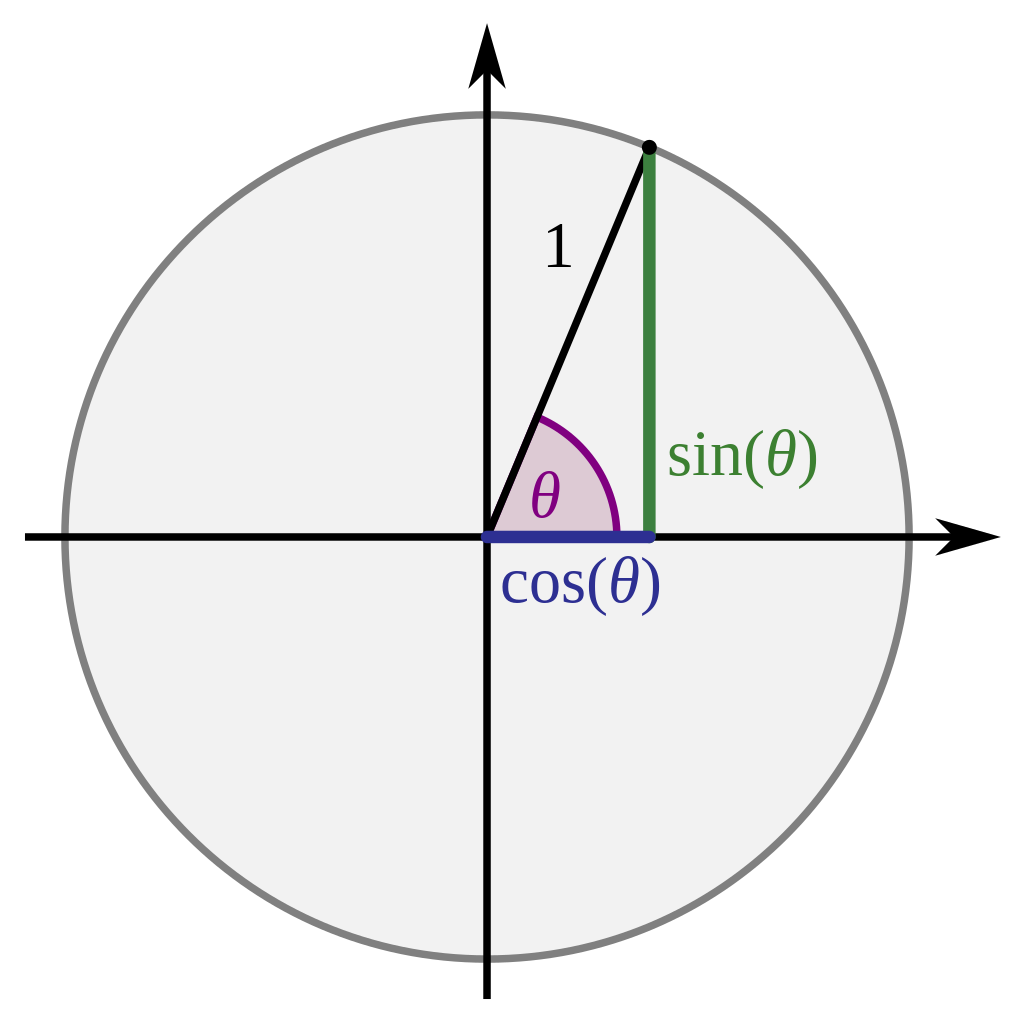
\includegraphics[width=\linewidth]{jednotkova_kruznice.png}
         \caption{Jednotková kružnice}
     \end{subfigure}
     \begin{subfigure}{0.65\textwidth}
         \centering
         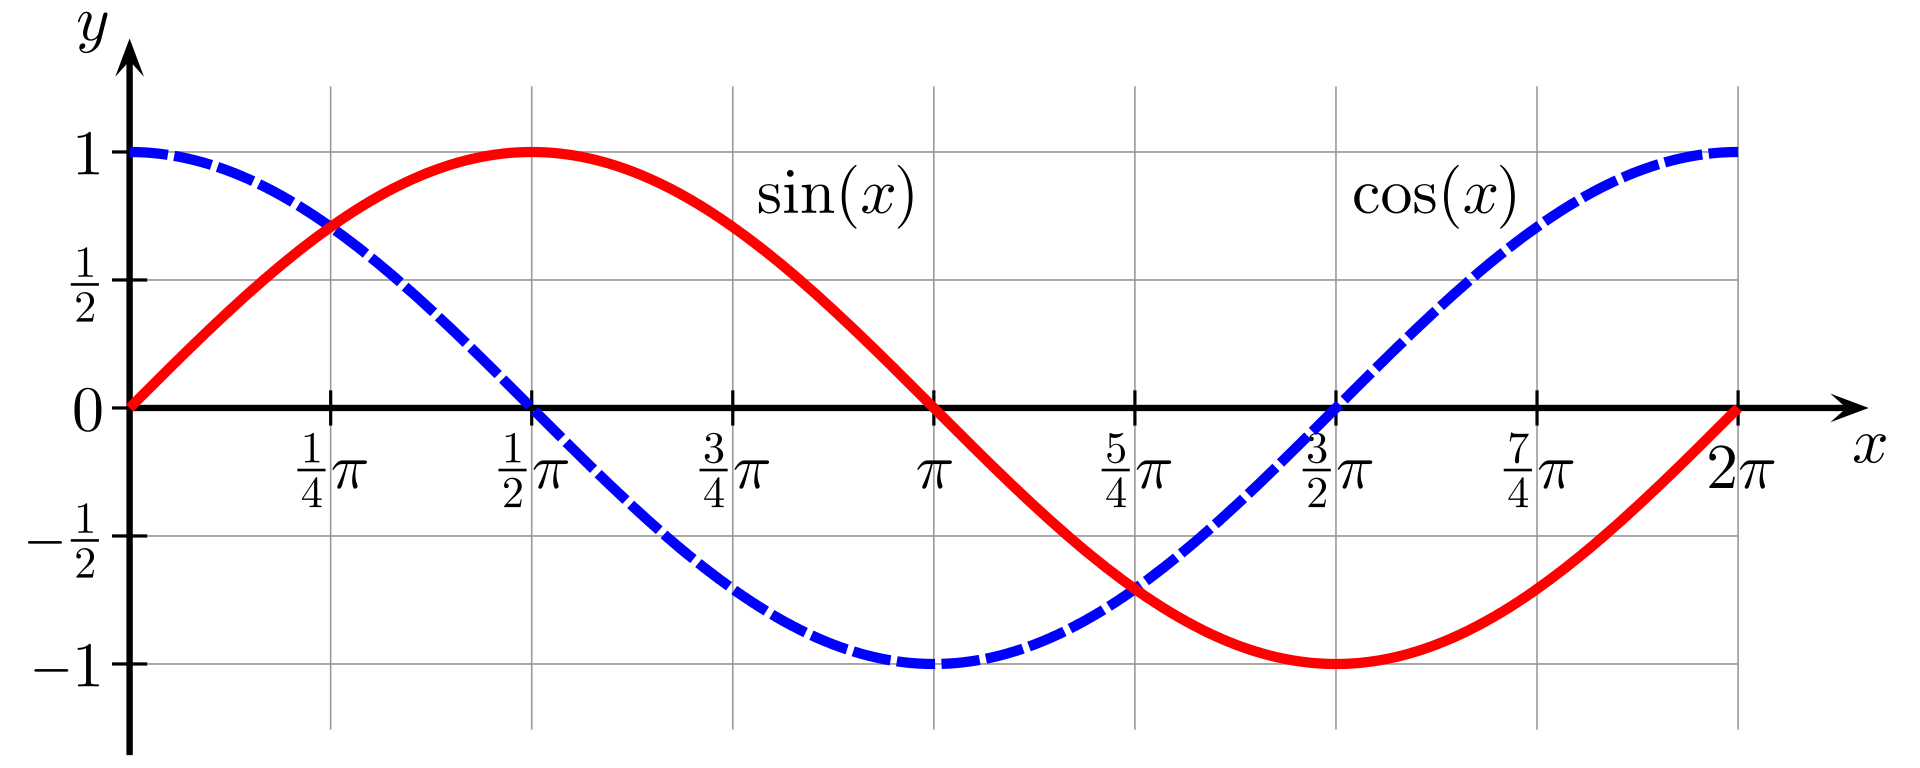
\includegraphics[width=\linewidth]{prubeh.png}
         \caption{Průběh funkcí $\sin$ a $\cos$}
     \end{subfigure}
     \caption{Funkce $\sin$ a $\cos$.}
\end{figure}

\begin{figure}[ht!]
     \centering
     \begin{subfigure}{0.49\textwidth}
         \centering
         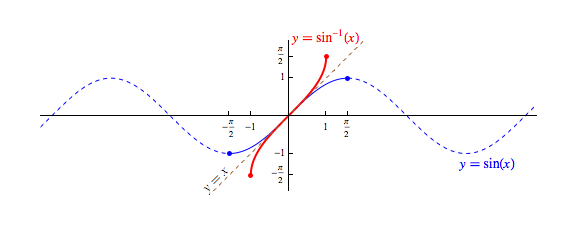
\includegraphics[width=\linewidth]{arcsine.png}
         \caption{Průběh funkce $\arcsin$}
     \end{subfigure}
     \begin{subfigure}{0.49\textwidth}
         \centering
         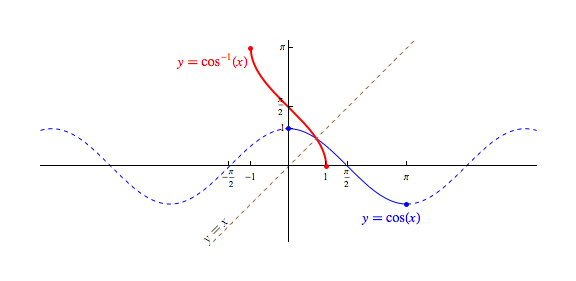
\includegraphics[width=\linewidth]{arccosine.png}
         \caption{Průběh funkce $\arccos$}
     \end{subfigure}
     \caption{Funkce $\arcsin$ a $\arccos$.}
\end{figure}

\begin{figure}[ht!]
     \centering
     \begin{subfigure}{0.49\textwidth}
         \centering
         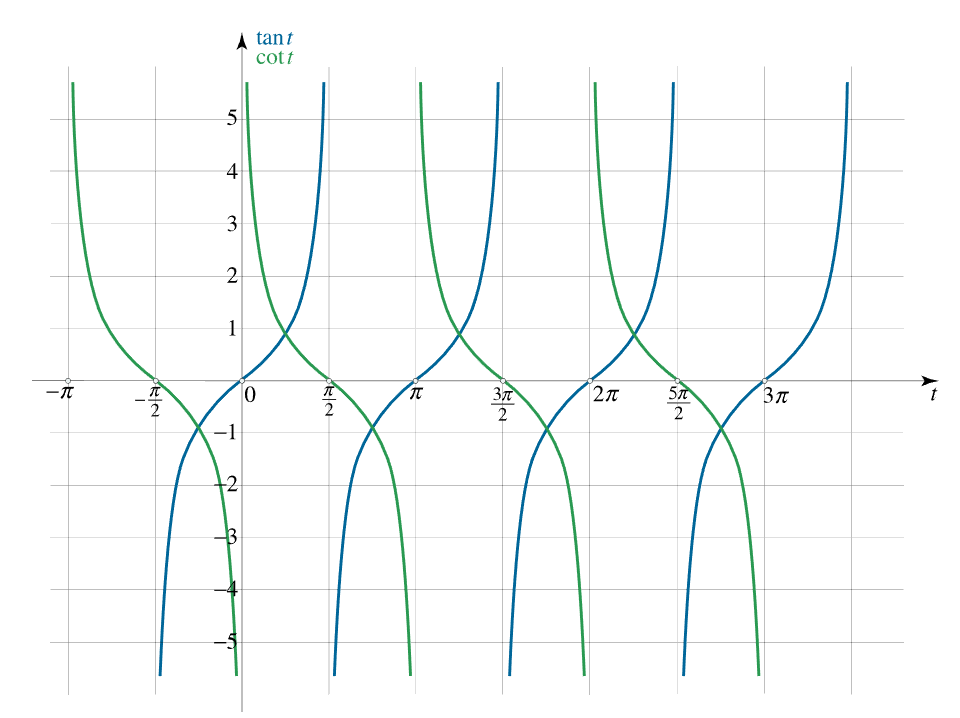
\includegraphics[width=\linewidth]{tgcotg.png}
         \caption{Průběh funkce $\tg$ a $\cotg$}
     \end{subfigure}
     \begin{subfigure}{0.49\textwidth}
         \centering
         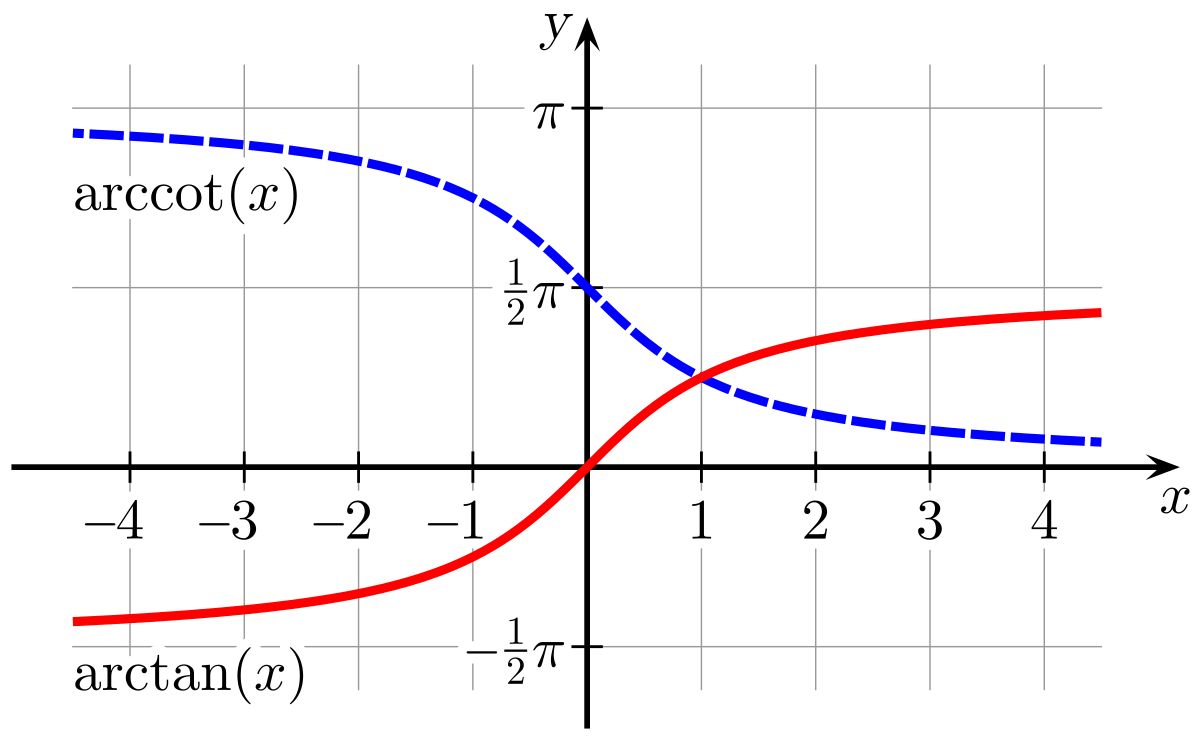
\includegraphics[width=\linewidth]{arctg_arccotg.png}
         \caption{Průběh funkce $\arctg$ a $\arccotg$}
     \end{subfigure}
     \caption{Funkce $\tg$ a $\cotg$.}
\end{figure}

\begin{figure}[ht!]
     \centering
     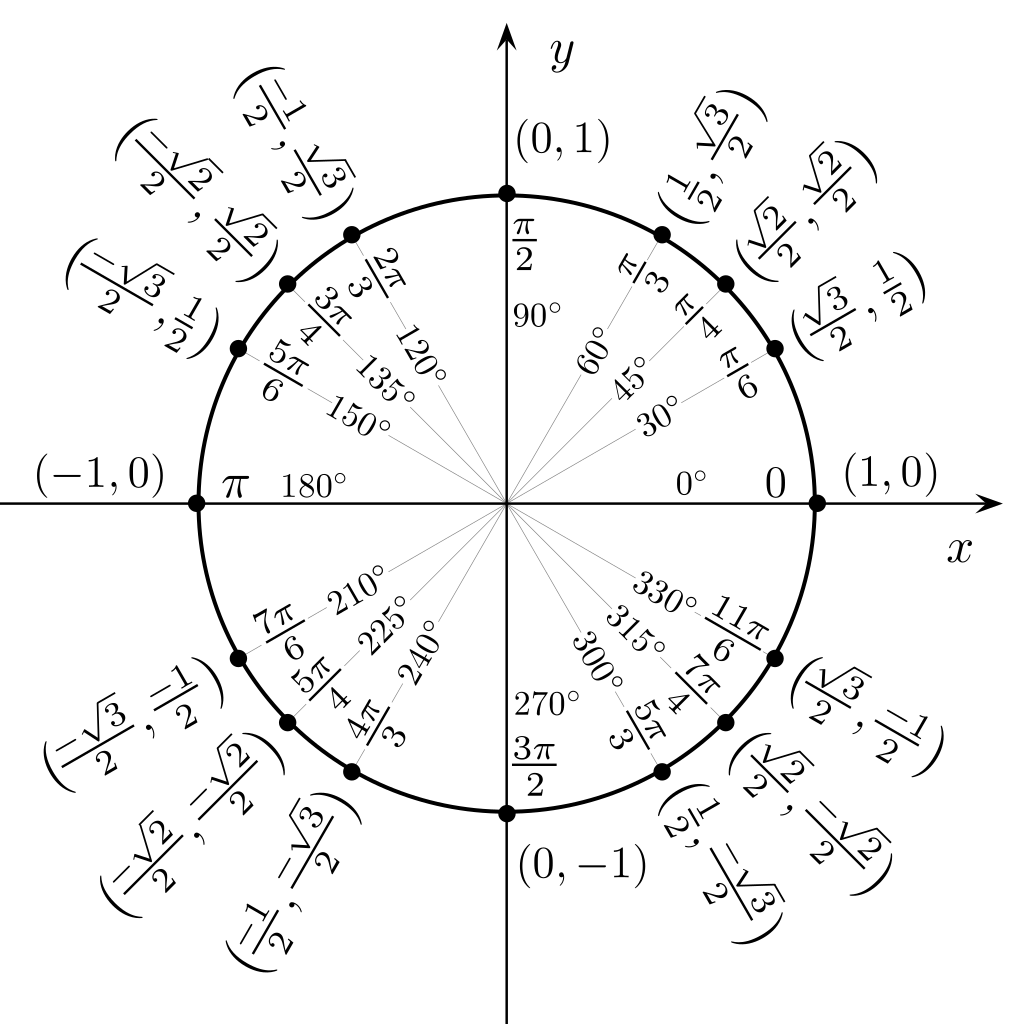
\includegraphics[width=0.6\linewidth]{jedn_k_s_hodn.png}
     \caption{Jednotková kružnice s hodnotami $(\cos \varphi, \sin \varphi).$}
     \label{kruzsh}
\end{figure}

\begin{figure}[ht!]
     \centering
     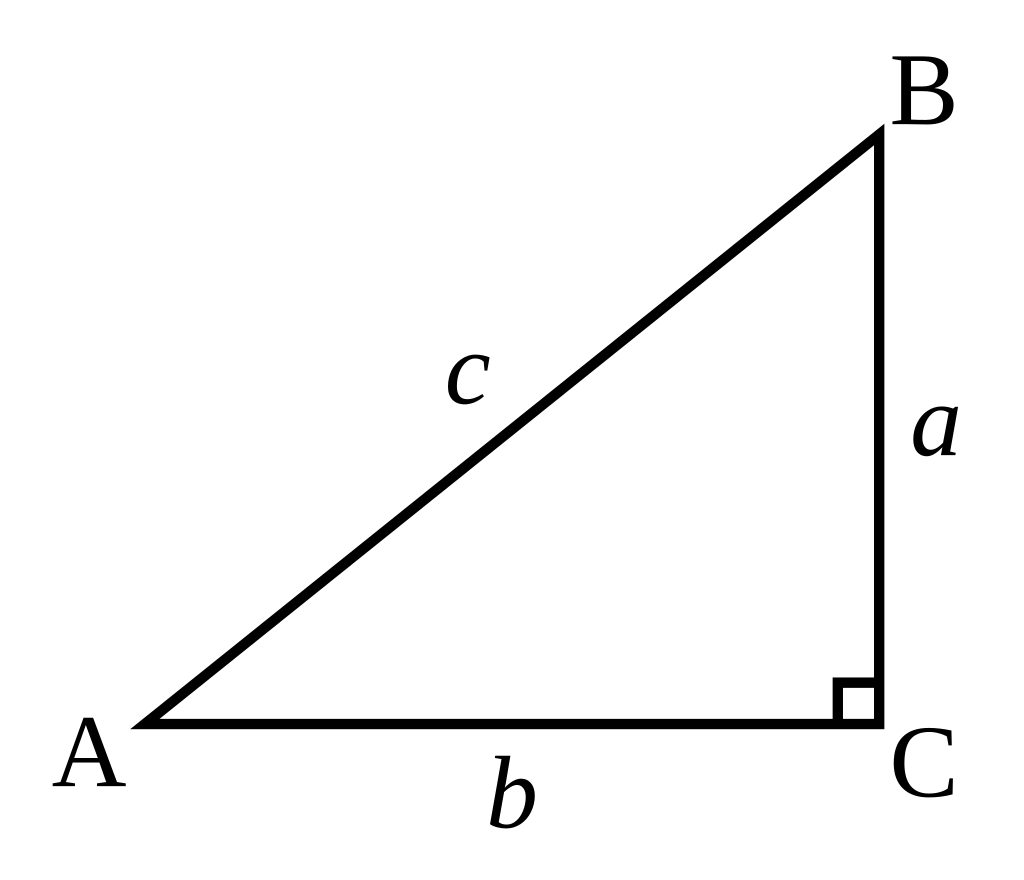
\includegraphics[width=0.3\linewidth]{right_t.png}
     \caption{Pravoúhlý trojúhelník s přeponou $c.$}
     \label{prav_t}
\end{figure}

\pagebreak

\begin{pozn}
    \par V obrázku \ref{kruzsh} jsou uvedeny hodnoty funkcí sinus a kosinus ve tvaru
    komplexního čísla, víme totiž
    $$ a = | a | \cdot (\cos \varphi + i\mkern1mu \sin \varphi)$$
    pro nějaké $a \in \mathbb C.$ Jelikož se jedná o jednotkovou kružnici, kde platí
    $|a| = 1,$ máme
    $$a=\cos \varphi +i\mkern1mu \sin \varphi. $$
    Pokud chápeme komplexní číslo jako uspořádanou dvojici $(k,l)=k+i\mkern1mu l,$
    dobereme se k~zápisu, jenž je použit v obrázku.
    \par Všimněme si navíc, že platí
    $$k^2+l^2=1 \,\,\,\,\,\, \forall (k,l).$$
\end{pozn}

\begin{pozn}
    V obrázku \ref{prav_t} platí pro úhel $\alpha = \sphericalangle BAC:$
    \begin{enumerate}[$i.$]
        \item $\sin \alpha= \frac{a}{c},$
        \item $\cos \alpha= \frac{b}{c},$
        \item $\tg \alpha= \frac{a}{b},$
        \item $\arctg \alpha= \frac{b}{a}.$
    \end{enumerate}
\end{pozn}

\begin{pozn}[Základní hodnoty goniometrických funkcí]\,\\
    \begin{tabularx}{\textwidth}{| p{0.087\textwidth} || p{0.081\textwidth} | p{0.081\textwidth} |
    p{0.081\textwidth} | p{0.081\textwidth} | p{0.081\textwidth} | p{0.081\textwidth} | p{0.081\textwidth}
    | p{0.081\textwidth} |}
    \hline
    $\beta$ [$^\circ$] & 0 & 30 & 45 & 60 & 90 & 180 & 270 & 360 \\
    \hline
    $\alpha$ [rad] & 0 & $\frac{\pi}{6}$ & $\frac{\pi}{4}$ & $\frac{\pi}{3}$ & $\frac{\pi}{2}$ & $\pi$ & $\frac{3\pi}{2}$ & $2\pi$\\
    \hline
    $\sin \alpha$ & 0 & $\frac{1}{2}$ & $\frac{\sqrt{2}}{2}$ & $\frac{\sqrt{3}}{2}$ & 1 & 0 & $-1$ & 0\\
    \hline
    $\cos \alpha$ & 1 & $\frac{\sqrt{3}}{2}$ & $\frac{\sqrt{2}}{2}$ & $\frac{1}{2}$ & 0 & $-1$ & 0 & 1\\
    \hline
    $\tg \alpha$ & 0 & $\frac{\sqrt{3}}{3}$ & 1 & $\sqrt{3}$ & -- & 0 & -- & 0\\
    \hline
    $\cotg \alpha$ & -- & $\sqrt{3}$ & 1 & $\frac{\sqrt{3}}{3}$ & 0 & -- & 0 & --\\
    \hline
    \end{tabularx}
\end{pozn}

\begin{pozn}
    Pro zajímavou animaci viz \href{https://upload.wikimedia.org/wikipedia/commons/3/3b/Circle_cos_sin.gif}{tento odkaz}.
\end{pozn}

\begin{pozn}
    Očividně platí následující věty (plyne z grafů jednotlivých funkcí nebo přímo z definice).
\end{pozn}

\begin{veta}
  $\forall x \in \mathbb{R}:$
  \begin{enumerate}[$i.$]
    \item $\sin x = \cos \left(x- \frac{\pi}{2}\right)=-\cos\left(x+\frac{\pi}{2}\right)$,
 	\item $\cos x = \sin \left(x+\frac{\pi}{2}\right)=-\sin \left(x- \frac{\pi}{2} \right)$.
  \end{enumerate}
\end{veta}

\begin{veta}
  $\forall x \in \mathbb{R}\smallsetminus\bigcup_{k\in \mathbb Z} \left \{ \frac{k\pi}{2} \right \} :$
  \begin{enumerate}[$i.$]
    \item $\tg x = -\cotg \left ( x- \frac{\pi}{2} \right )$,
 	\item $\cotg x = -\tg \left ( x- \frac{\pi}{2} \right )$.
  \end{enumerate}
\end{veta}

\begin{veta}
  $\forall x \in \mathbb{R}\smallsetminus\bigcup_{k\in \mathbb Z} \left \{ \frac{k\pi}{2} \right \}: \tg x \cdot \cotg x = 1.$
\end{veta}

\begin{pozn}
    Funkce sinus a kosinus lze také definovat předpisy
    \begin{align*}
        \sin x & = \sum_{n=0}^\infty (-1)^n \frac{x^{2n+1}}{(2n+1)!},\\
        \cos x & = \sum_{n=0}^\infty (-1)^n \frac{x^{2n}}{(2n)!},
    \end{align*}
    kde $x \in \mathbb R.$
\end{pozn}


\nocite{*}
\clearpage
{\small\bibliography{references}}

\backmatter
%!TEX root = ../main.tex

\clearpage
\phantomsection
\addcontentsline{toc}{section}{About the Author}
\begin{adjustwidth}{0.1\textwidth}{0.1\textwidth}
\begingroup
\null\vspace{0.2\textheight}
\begin{center}
{\bfseries\Large O autorovi}\par\vspace{2em}

Da, da, da, da, da \\
It's the motherfucking D-O-double-D \\
Da, da, da, da, da \\
You know I'm mobbin' with Honza Romanovský (Yeah, yeah, yeah)
\end{center}
\endgroup
\end{adjustwidth}
\clearpage


\end{document}
